\documentclass[11pt]{report}
\usepackage{etex}
\usepackage[
    paper=letterpaper,
    top=1.125in, 
    bottom=1.25in, 
    left=1.25in, 
    right=1.25in,
    %includefoot,            % Uncomment to put page number above margin
    %marginparwidth=1in,     % Length of section titles
    %marginparsep=.05in,     % Space between titles and text
    ]{geometry}
\usepackage[pdftex]{graphicx}
\usepackage{amsmath,amssymb,latexsym}
\usepackage[style=numeric,sorting=nty]{biblatex}
\usepackage{tipa,textcomp,enumerate}
\usepackage{fancyhdr,tabularx,tabulary,diagbox}
\usepackage{paralist,comment,fancyvrb}
\usepackage{multirow,url,calc}
\usepackage[group-separator={,}]{siunitx}
\usepackage{pgfplots,xmpincl}
\usepackage{epstopdf}
\usepackage[nottoc,numbib]{tocbibind}
\usepackage{color,colortbl}
\usepackage{draftwatermark}
\usepackage{float,wrapfig,varioref}

\newcommand*\mean[1]{\overline{#1}}

\addbibresource{bibdata.bib}

\newcommand{\mtilde}{$\mathtt{\sim}$}
\usepackage{listings}% http://ctan.org/pkg/listings
\lstset{
  basicstyle=\ttfamily,
  mathescape
}

\SetWatermarkScale{3}

\usetikzlibrary{arrows.meta}
\usetikzlibrary{patterns}
\pgfplotsset{compat=1.12}

% use with tikz to create Normal distribution
\pgfmathdeclarefunction{gauss}{2}{%
  \pgfmathparse{1/(#2*sqrt(2*pi))*exp(-((x-#1)^2)/(2*#2^2))}%
}

\graphicspath{ {images/} }
\includexmp{metadata/CC_Attribution_4.0_International}

% to create matrices that represent games in normal form
% with better spacing for readability and with vertical lines
% that do not extend over all rows.
\newcommand{\gtcol}[1]{\multicolumn{1}{c|}{#1}}
\newcolumntype{Y}{>{\centering\arraybackslash}X}  % centered
\newcolumntype{Z}{>{\raggedleft\arraybackslash}X} % right-justify

\includecomment{solution}
%\excludecomment{solution} % comment this out to create the solutions
\newcommand{\bs}{\textbf{Solution.}~}

\setcounter{secnumdepth}{2}
\setcounter{tocdepth}{1}

\begin{document}
\chapter*{\Huge \center An Introduction to Prescriptive
  and Predictive Modeling}
\thispagestyle{empty}
%{\hspace{0.25in} \includegraphics{./ru_sun.jpg} }
\begin{center}
{\large Darin England\\
Department of Industrial and Systems Engineering\\
University of Minnesota, Minneapolis}
\end{center}

\newpage
\noindent
An Introduction to Prescriptive and Predictive Modeling\\
Copyright \copyright 2020 by Darin England\\
\includegraphics[scale=0.8]{by-nc.eps}\\
This work is licensed under the Creative Commons Attribution-NonCommercial 4.0
International License. To view a copy of this license,
visit \url{http://creativecommons.org/licenses/by-nc/4.0/}.
You are free to:\\
Share – copy and redistribute the material in any medium or format\\
Adapt – remix, transform, and build upon the material\\
The licensor cannot revoke these freedoms as long as you follow the license terms.
Under the following terms:\\
Attribution – You must give appropriate credit, provide a link to the license,
and indicate if changes were made. You may do so in any reasonable manner,
but not in any way that suggests the licensor endorses you or your use.\\
NonCommercial – You may not use the material for commercial purposes.\\
Although every precaution has been taken to verify the accuracy of the
information contained herein, the author and publisher assume no
responsibility for any errors or omissions. No liability is assumed
for damages that may result from the use of information contained
within.

\tableofcontents
\chapter*{Preface}
\addcontentsline{toc}{chapter}{Preface}

\subsubsection*{Goals} 

The book provides a practical introduction to the use of mathematical
modeling and statistical computing techniques to solve decision
problems that arise in various industrial settings. Examples are drawn
from manufacturing, finance, sports, healthcare, retail,
transportation, and other areas. In realistic settings, proficiency
with mathematical and statistical computing software is required to
solve these problems. We use the algebraic modeling language GAMS for
solving mathematical programming problems and we use the R programming
language for obtaining answers to statistical computing problems;
however, the methodologies that are developed stand on their own and
the book can be used with other programming langauges. GAMS code and
listings are provided via github in the gams/ directory. R code,
output, and discussion are provided in the form of Jupyter notebooks
in the src/ directory. The github repository for the book is
\url{https://github.com/bx549/IPPM}.  We hope that students as well as
practicing engineers and analysts will find the book to be useful.

\subsubsection*{Acknowledgments}

I want to acknowledge the following undergraduate students in the
Department of Industrial and Systems Engineering who created content
and checked solutions to end-of-chapter exercises.  Hannah Kleist
created scenarios for deterministic optimization problems in Chapter 1
and implemented solutions in GAMS. She also created content for
exercises on stochastic processes in chapter 2. Emily Sayles created
content for end-of-chapter exercises on deterministic inventory models
in chapter 1, probabilistic inventory models in chapter 2, and
decision problems in chapter 3. Braeden Greseth created content and
implemented solutions in R for exercises in chapters 2, 4, and 5.

\chapter{Prescriptive Modeling}
\section{Linear Programming}

% this section needs to be re-written
\emph{A Resource Allocation Problem.} This example is taken 
from~\cite{chvatal:1983}.  A forester has 100
acres of hardwood timber. She also has \$4000 cash on-hand to use for
the forestry business. There are two possible courses of action to 
take with the 100 acres of available hardwood:
\begin{enumerate}
\item Harvest the hardwood and let the area naturally regenerate. This
  would cost \$10 per acre now and return \$50 per acre later,
  yielding a profit of \$40 per acre.
\item Harvest the hardwood and plant the area with pine. This would
  cost \$50 per acre now and return \$120 per acre later, yielding a
  profit of \$70 per acre. \label{d2}
\end{enumerate}
Option \ref{d2} is clearly more profitable; however, the forester must
respect her budget of \$4000. The mathematical programming problem is
to maximize total profit subject to the resource constraints, which
are the acres of available hardwood and the budget.

The complete problem formulation in AMPL is shown in
figure~\ref{forest}.  Two decision variables, \texttt{x1} and
\texttt{x2}, represent the number of acres that the forester should
allocate to each of the two possible courses of action.  It would make
no sense to allow these decision variables to take on negative
values. The non-negativity requirements are more cleanly specified
directly in the variable declarations as opposed to creating separate
constraints. A graphical depiction of the feasible solution space is
shown in figure~\ref{feasibleregion}.

\begin{SaveVerbatim}{vrbforest}
var x1 >= 0;  # acres to fell and let regenerate
var x2 >= 0;  # acres to fell and plant with pine

maximize profit: 40*x1 + 70*x2;

s.t. acres: x1 + x2 <= 100;
s.t. budget: 10*x1 + 50*x2 <= 4000;
\end{SaveVerbatim}

\begin{figure}
\fbox{
\begin{minipage}{\textwidth}
\BUseVerbatim{vrbforest}
\caption{Forestry problem (\texttt{forester.mod})}
\label{forest}
\end{minipage}
}
\end{figure}

\begin{figure}
\begin{center}
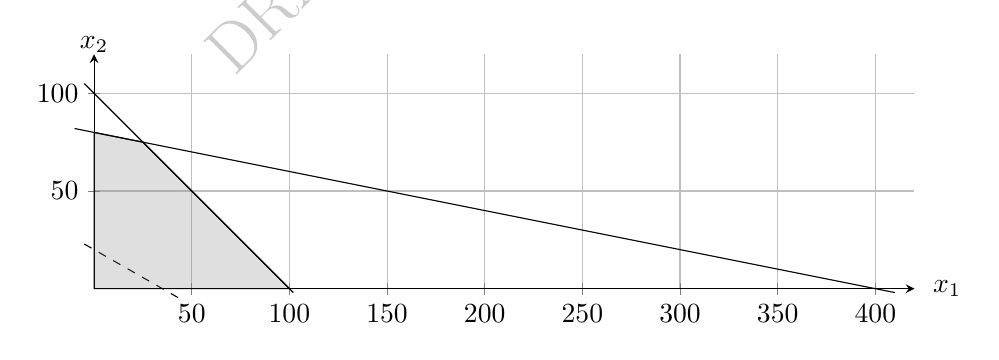
\begin{tikzpicture}
  \begin{axis}[ width=12cm,
    unit vector ratio*=1 1 1,
    enlargelimits=false,
    grid=both,
    axis x line=middle,
    axis y line=middle,
    title=,
    clip=false,
    ymin=0, ymax=120,
    xmin=0, xmax=420 ]

    \addplot[domain=-10:410] {80 - .2*x};
    \addplot[domain=-5:102] {100 - x};
    \addplot[domain=-5:45,dashed] {20 - .57143*x};
    \addplot[fill=gray, fill opacity=.25]
    coordinates { (0,0) (100,0) (25,75) (0,80) }\closedcycle;

  % to get axis labels at the end of the axis
  \node at (axis description cs:1.04,0) {$x_1$}; \node at
  (axis description cs:0,1.04) {$x_2$};
\end{axis}
\end{tikzpicture}
\end{center}
\caption{Feasible Region for the Forestry Problem}
\label{feasibleregion}
\end{figure}

The constraints labeled \texttt{acres} and \texttt{budget} represent
the limitations on available resources.  It's unnecessary to
explicitly name constraints in AMPL; however, providing short,
descriptive names aids interpretation of the model. Moreover, in a
resource allocation problem such as this, the constraint names refer
to the values of the associated dual variables, which have an economic
interpretation as the marginal value of an additional unit of the
resource.

This problem is small enough that we can include all data parameters
directly in the model specification. Although we will not cover it in
this quick start guide, it is good practice to separate the data from
the model, and AMPL encourages this separation by providing
\texttt{param} declarations and the ability to have a separate
\texttt{data} section. Indeed, it's hard to understand the benefit of
an algebraic modeling language unless you are working on a large
problem.  It's worth noting that AMPL doesn't actually solve the
mathematical programming problem, but rather passes a description of
the problem to a solver, which returns information about the solution
(if any solution was found) to AMPL. An AMPL session for the forestry
problem follows:

\begin{Verbatim}[samepage=true]
ampl: model forester.mod;
ampl: solve;
MINOS 5.5: optimal solution found.
2 iterations, objective 6250
ampl: display x1,x2;
x1 = 25
x2 = 75
\end{Verbatim}

The optimal solution indicates that the forester should let 25 acres
of the hardwood regenerate naturally and plant 75 acres with pine, for
a total profit of \$6250. Notice that the entire budget of \$4000 is
exhausted because $10 \times 25 + 50 \times 75 = 4000$. When a
resource capacity constraint such as \texttt{acres} or \texttt{budget}
holds with equality in the optimal solution (as in this example), then
the constraint is \emph{binding}; all of the resource associated with
the constraint is being consumed. If more/less of the resource were
available, then profit would be increased/decreased. The value of the
associated dual variable indicates the amount by which profit would be
affected for small changes in the supply of the resource. This is
called the marginal value of a resource, or the shadow price.

\begin{Verbatim}[samepage=true]
ampl: display acres, budget;
acres = 32.5
budget = 0.75
\end{Verbatim}

In AMPL the name of a constraint is used to refer to the associated
dual variable. Displaying the shadow prices for the forester problem
indicates that an additional acre of hardwood timber would increase
profit by \$32.50, given the same budget of \$4000.  Modifying the
right-hand side of \texttt{acres} to 101 and re-solving shows that
this is indeed the case.

\begin{Verbatim}[samepage=true]
ampl: reset;
ampl: model forester.mod;
ampl: expand acres;
subject to acres:
	x1 + x2 <= 101;

ampl: solve;
MINOS 5.5: optimal solution found.
2 iterations, objective 6282.5
ampl: display x1,x2;
x1 = 26.25
x2 = 74.75
\end{Verbatim}

The \texttt{expand} command displays the full form of a set of
constraints.  (This will be useful for indexed expressions.) Notice
that the values of the decision variables have necessarily changed and
that the solution is no longer integer-valued.  This is typical of
resource allocation problems. We are in fact assuming that the
forester is able to execute the decisions on partial acres.  For the
\texttt{budget} constraint, an additional one dollar increase/decrease
in the right-hand side would increase/decrease profit by \$0.75, given
the same 100 acres of hardwood. It stands to reason, then, that the
forester could take out a loan and apply the funds to her
operation. As long as the interest rate is less than .75, profit will
increase.

Shadow prices are valid for \emph{limited} increases/decreases in the
right-hand sides of the constraints. The ranges over which the these
values are valid is a topic of sensitivity analysis. Here, we will
show how to extract this information from AMPL. First we need to tell
AMPL to use a solver that is able to return sensitivity information
along with the optimal solution. We will instruct AMPL to use the solver
\texttt{gurobi}. Then we set a solver-specific option to make the
sensitivity range information available.

\begin{Verbatim}[samepage=true]
ampl: reset;
ampl: model forester.mod;
ampl: option solver gurobi;
ampl: option gurobi_options 'solnsens 1'; 
ampl: solve;
Gurobi 8.1.0: solnsens 1
Gurobi 8.1.0: optimal solution; objective 6250

suffix sensublo OUT;
suffix sensubhi OUT;
suffix sensobjlo OUT;
suffix sensobjhi OUT;
suffix senslblo OUT;
suffix senslbhi OUT;
suffix sensrhslo OUT;
suffix sensrhshi OUT;
\end{Verbatim}

We are now able to display the ranges over which the current shadow
prices of \$32.5 per acre and \$0.75 per dollar of budget are
valid. To do this we simply add a suffix to the name of the
constraint, separated by a ``\texttt{.}''. The suffix
\texttt{.sensrhslo} displays the lower limit of a constraint's
right-hand side, while \texttt{.sensrhshi} displays the upper limit.
In the AMPL session follows, the
upper limit of 5000 on the right-hand side of \texttt{budget}
indicates the forester should only consider loans of \$1000 or less to
be valued at an incremental marginal value of 0.75.

\begin{Verbatim}[samepage=true]
ampl: display acres.sensrhslo, acres.sensrhshi;
acres.sensrhslo = 80
acres.sensrhshi = 400

ampl: display budget.sensrhslo, budget.sensrhshi;
budget.sensrhslo = 1000
budget.sensrhshi = 5000
\end{Verbatim}

Sensitivity ranges may also be obtained for the decision variables. In
this case the lower and upper limits represent the valid ranges on the
objective function coefficients over which the current solution
remains optimal.  The suffixes \texttt{.sensobjlo} and
\texttt{.sensobjhi} are used to refer to these lower and upper limits.
Displaying this information for the forestry problem reveals that the
current solution value of \texttt{x1 = 25} remains optimal as long as
its coefficient in the objective function is in the range 14 to 70,
holding all other parameters at their current values.

\begin{Verbatim}[samepage=true]
ampl: display x1.sensobjlo, x1.sensobjhi;
x1.sensobjlo = 14
x1.sensobjhi = 70

ampl: display x2.sensobjlo, x2.sensobjhi;
x2.sensobjlo = 40
x2.sensobjhi = 200
\end{Verbatim}

The other suffixes, \texttt{.senslblo}, \texttt{.senslbhi},
\texttt{.sensublo}, and \texttt{.sensubhi}, refer to ranges on the
values (not the coefficients) of the decision variables over which the
current basis remains optimal. We will not use these suffixes.

\section{Integer Programming}

\section{Dynamic Programming}

\section{Inventory Models}

\section{Exercises}
\begin{enumerate}

% written by Hannah
\item \emph{Feasible region for an LP.} Indicate graphically whether each of the following
  linear programs has a feasible solution. Graphically determine the
  optimal solution, if one exists, or show that no optimal solution
  exists.

\begin{enumerate}
\item
\[
  \begin{array}{lrrrrr}
    \textrm{maximize}   & x_1& +& 3x_2&  & \\
    \textrm{subject to} & x_1& -&4x_2& \leq & 4  \\
                        & x_1& +& 2x_2& \leq & 4 \\
    \multicolumn{3}{r}{x_1,x_2}&       \geq & 0 
  \end{array}
\]

\item
\[
  \begin{array}{lrrrrr}
    \textrm{minimize}   & x_1& +& 2x_2&  & \\
    \textrm{subject to} & 2x_1& -&x_2& \leq & 3  \\
                        & 2x_1& -& x_2& \geq & -3 \\
    \multicolumn{3}{r}{x_1,x_2}&       \geq & 0 
  \end{array}
\]

\end{enumerate}

\begin{solution}
\bs The feasible region for the linear program in part a) is shown
below. The objective function is plotted as a dashed line. The
optimal solution occurs at $x_1=0$, $x_2=2$, and value of the
objective function at the optimal solution is $z=6$.

\begin{center}
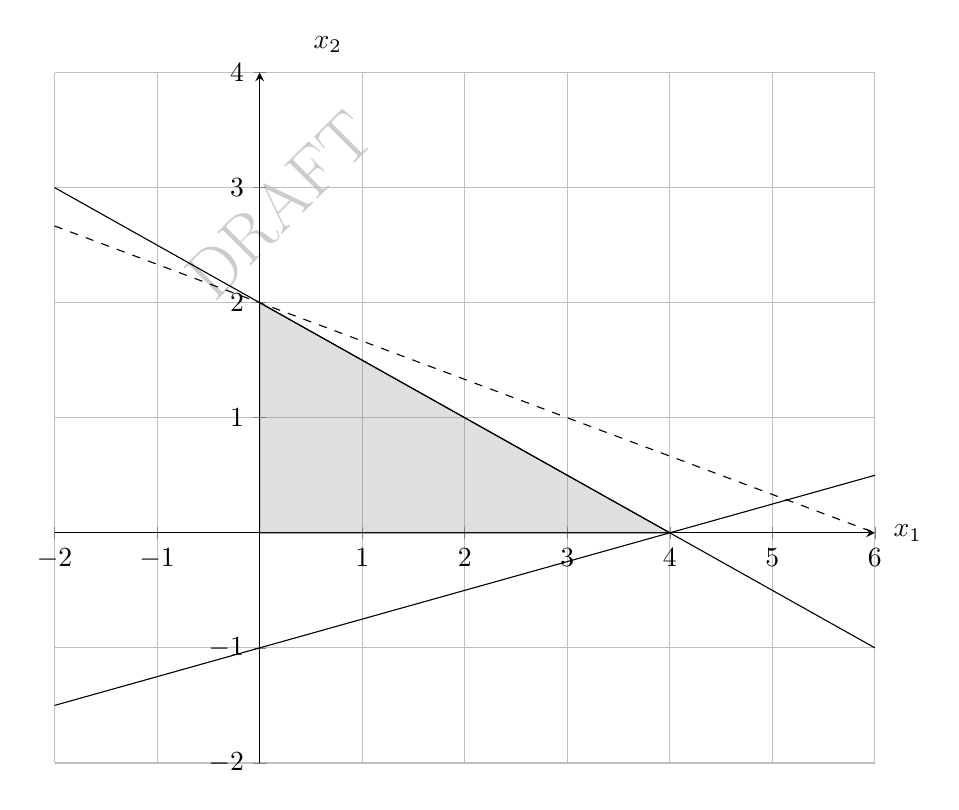
\begin{tikzpicture}
  \begin{axis}[ width=12cm, grid=both, axis x line=middle, axis y
    line=middle, title=, clip=false, ymin=-2, ymax=4, xmin=-2,
    xmax=6 ]

    \addplot[domain=-2:6] {-1 + 1/4*x}; \addplot[domain=-2:6] {2
      - 1/2*x}; \addplot[domain=-2:6,dashed] {2 - 1/3*x};
    \addplot[fill=gray, fill opacity=.25] coordinates { (0,0)
      (4,0) (0,2) }\closedcycle;

    % to get axis labels at the end of the axis
    \node at (axis description cs:1.04,.333) {$x_1$}; \node at
    (axis description cs:.333,1.04) {$x_2$};
  \end{axis}
\end{tikzpicture}
\end{center}

The feasible region for the linear program in part b) is unbounded;
however, since it is a minimization problem, it has an optimal
solution at $x_1=0$, $x_2=0$. The value of the objective function at
the optimal solution is $z=0$.

\begin{center}
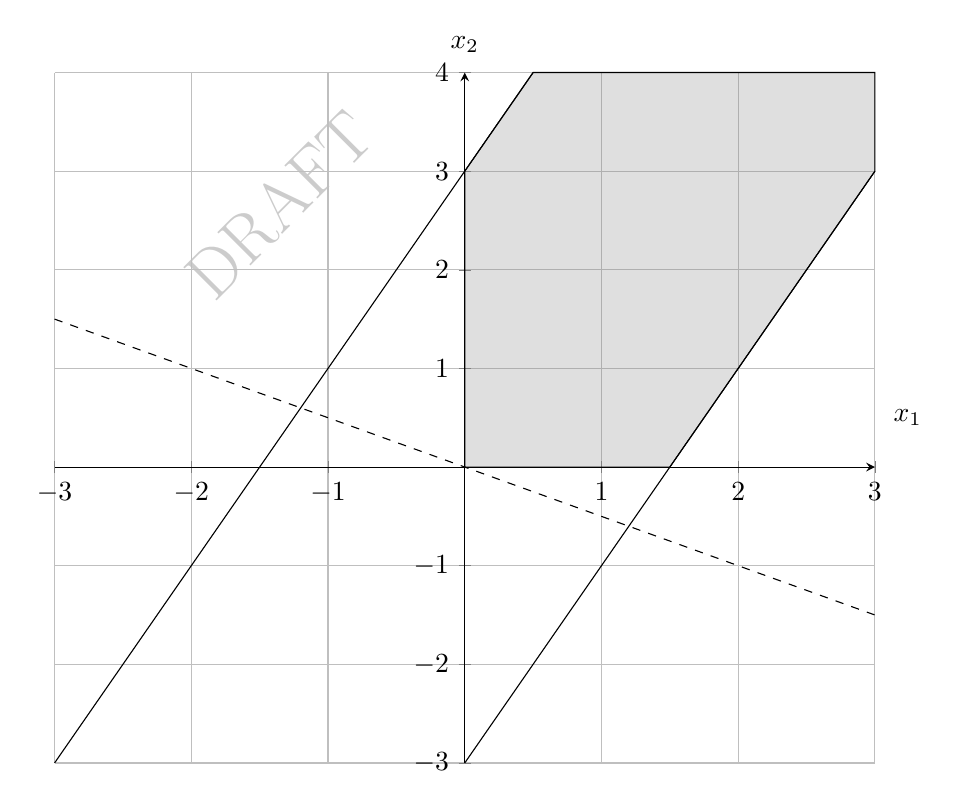
\begin{tikzpicture}
  \begin{axis}[ width=12cm, grid=both, axis x line=middle, axis y
    line=middle, title=, clip=false, ymin=-3, ymax=4, xmin=-3,
    xmax=3 ]

    \addplot[domain=0:3] {-3 +2*x}; \addplot[domain=-3:.5] {3+2*x};
    \addplot[domain=-3:3,dashed] {-1/2*x}; \addplot[fill=gray, fill
    opacity=.25] coordinates { (0,0) (0,3) (.5,4) (3,4) (3,3) (1.5,0)
    }\closedcycle;

    % to get axis labels at the end of the axis
    \node at (axis description cs:1.04,.5) {$x_1$}; \node at (axis
    description cs:.5,1.04) {$x_2$};
  \end{axis}
\end{tikzpicture}
\end{center}

\end{solution}

% this exercise needs to be re-written
\item \emph{Resource allocation to maximize profit.} 
At the Ma-and-Pa grocery store, shelf space is limited
  and must be used effectively to increase profit. Two cereal items,
  Grano and Wheatie, compete for a total shelf space of 60 ft$^2$. A
  box of Grano occupies .2 ft$^2$ and a box of Wheatie requires .4
  ft$^2$. The maximum daily demands for Grano and Wheatie are 200 and 120
  boxes, respectively. A box of Grano nets \$1.00 in profit, while a
  box of Wheatie nets \$1.35. Ma and Pa think that because the unit
  profit of Wheatie is 35\% higher than that of Grano, Wheatie should
  be allocated 35\% more space than Grano, which amounts to allocating
  about 57\% to Wheatie and 43\% to Grano. What do you think?
  (You can solve this problem however you like, but you must provide
  the allocation of shelf space that maximizes profit.)
  

\begin{solution}
\bs My AMPL model and output follow. The solution indicates that more
space should be allocated to Grano than Wheatie. This is because
the profit per square foot is larger. The solution indicates that
Ma and Pa should stock 200 boxes of Grano and 50 boxes of Wheatie.

\begin{Verbatim}[samepage=true]
var x1 >=0, <= 200;   # boxes of grano
var x2 >= 0, <= 120;  # boxes of wheatie

maximize profit: x1 + 1.35*x2;
s.t. space: .2*x1 + .4*x2 <= 60;

ampl: model '/home/darin/Dropbox/isye/ie1101/hw/ma-and-pa-store.mod';
ampl: solve;
MINOS 5.51: optimal solution found.
2 iterations, objective 267.5
ampl: display x1, x2;
x1 = 200
x2 = 50
\end{Verbatim}
\end{solution}

% this problem needs to be re-written and GAMS code needs to be added.
\item \emph{A network flow problem.}
The U.S. government is auctioning oil leases at two sites, A and B. At
each site, 100,000 acres are to be auctioned. Three people are bidding
as follows.

\begin{tabular}{crr}
Bidder & site A & site B \\ \hline
Marshall & \$1000/acre & \$2000/acre \\
Ewing     & \$900/acre & \$2200/acre \\
Pickens  & \$1100/acre & \$1900/acre
\end{tabular}

The rules are that no bidder can receive more than 40\% of the land
being auctioned (i.e. the total amount of land being auctioned at
\emph{both} sites).
\begin{compactenum}
  \item Draw a diagram of the problem as a network flow model.
  \item Formulate a linear programming model to maximize the
    government's revenue.
  \item Solve the problem using optimization software.
\end{compactenum}

\begin{solution}
  \bs A diagram of the network flow model is shown below. Bidders 1, 2,
  and 3 correspond to Marshall, Ewing, and Pickens, respectively.
\vspace{.2in}
\begin{center}
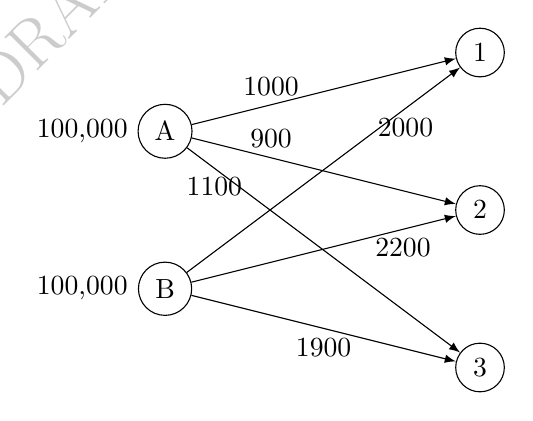
\begin{tikzpicture}[>=latex] % to get latex arrowheads

  \node[circle,draw](B) at (0,2) {B};
  \node[circle,draw](A) at (0,4) {A};
  \node[circle,draw](3) at (4,1) {3};
  \node[circle,draw](2) at (4,3) {2};
  \node[circle,draw](1) at (4,5) {1};

  \draw[->] (A) -- (1) node[above,pos=.3]{1000};
  \draw[->] (A) -- (2) node[above,pos=.3]{900};
  \draw[->] (A) -- (3) node[below,pos=.1]{1100};
  \draw[->] (B) -- (1) node[below,pos=.8]{2000};
  \draw[->] (B) -- (2) node[below,pos=.8]{2200};
  \draw[->] (B) -- (3) node[below,pos=.5]{1900};

  \node[anchor=east] at (A) {100,000~~~~};
  \node[anchor=east] at (B) {100,000~~~~};

\end{tikzpicture}
\end{center}

Let $x_{ij}$ be the amount of land bidder $j$ receives for site $i$.
  \[
     i \in \{\text{A},\text{B}\} \qquad j \in \{1,2,3\}
  \]
  The problem formulation is
\[
  \begin{array}{lrrrrrrrrrr}
    \textrm{maximize} &&&&&&&&&&\\   
    1000x_{\text{A}1}&+& 900x_{\text{A}2}&+&1100x_{\text{A}3}&+&2000x_{\text{B}1}&+&2200x_{\text{B}2}&+&1900x_{\text{B}3} \\ \\
    \textrm{subject to}  &&&&&&&&&&\\
    & & & & x_{\text{A}1}&+ & x_{\text{A}2}&+ &x_{\text{A}3} & = & 100,000 \\
    & & & & x_{\text{B}1}&+ & x_{\text{B}2}&+ &x_{\text{B}3} & = & 100,000 \\
    & & & & & &  x_{\text{A}1} & + & x_{\text{B}1} & \leq & 80,000 \\
    & & & & & &  x_{\text{A}2} & + & x_{\text{B}2} & \leq & 80,000 \\
    & & & & & &  x_{\text{A}3} & + & x_{\text{B}3} & \leq & 80,000 \\
    \multicolumn{11}{r}{x_{ij} \geq 0 \quad \text{for}~i \in \{\text{A},\text{B}\},~j \in \{1,2,3\} }
  \end{array}
\]

The optimal solution
is: bidder 1 (Marshall) receives 20,000 acres at site A and 20,000
acres at site B, bidder 2 (Ewing) receives 80,000 acres at site B, and
bidder 3 (Pickens) receives 80,000 acres at site A. The government
receives \$324 million in revenue.
\end{solution}


\end{enumerate}

\chapter{Probabilistic Models}

\section{Modeling with Probability Distributions}

% a discussion on binomial distribution.
The normal rate of infection of a certain disease in cattle is
25\%.  Each animal becomes infected (or not) independently of other
animals.  A team of veterinarians would like to test a new
vaccine. Which of the following two scenarios, \ref{sc1} or \ref{sc2},
provides more evidence that the vaccine is effective.  \emph{Hint:}
Compute the probability that each scenario would occur under the
hypothesis that the vaccine has no effect whatsoever.
\begin{enumerate}[A)]
\item 10 animals are vaccinated and none of them become infected. \label{sc1}
\item 17 animals are vaccinated. At most one of the animals becomes infected. \label{sc2}
\end{enumerate}

Let $X$ be the number of animals infected under the assumption that
the vaccine is worthless.  Under scenario \ref{sc1},
\[ X \sim \text{Binomial}(n=10,p=.25) \]
\[ P(X = 0) = {10 \choose 0} .25^0 .75^{10} = .0563 \]
Under scenario \ref{sc2}, 
\[ X \sim \text{Binomial}(n=17,p=.25) \]
\begin{align*} P(X \leq 1) &= P(X=0) + P(X=1) \\
                 &= \sum_{x=0}^1 {17 \choose x} .25^x .75^{17-x} \\
                 &= .0501
\end{align*}
In the absence of a working vaccine, scenario \ref{sc2} is less likely to occur,
and so it provides a better test of the effectiveness of the vaccine.


% use this section to illustrate modeling with a poisson rv
At a facility that manufactures recreational sports
  vehicles (ATVs), each vehicle is subjected to a final
  inspection. The rate of defects during final inspection is
  $\lambda=1.5$ defects per vehicle.
\begin{enumerate}
\item What is an appropriate probability distribution to model the
number of defects? \label{atv1}
\item What proportion of vehicles have more than 2 defects? \label{atv2}
\item Management has set a new goal that the proportion
of vehicles with no defects is .5. What rate $\lambda$ would
achieve this goal? \label{atv3}
\end{enumerate}

We are interested in the number of defects, which is discrete.
The Poisson distribution makes sense because it is commonly used
for count data. Moreover, we are given information for a single
parameter, and the Poisson distribution has a single parameter.
If we let the random variable $X$ represent the number of defects
per vehicle, then a reasonable distribution is
\[ X \sim \text{Poisson}(\lambda=1.5) \]
For part~\ref{atv2},
\begin{align*}
P(X>2) &= 1 - P(X \leq 2)\\
       &= 1 - \sum_{x=0}^2 \frac{e^{-\lambda}\lambda^x}{x!}\\
       &= 0.191
\end{align*}
For part \ref{atv3}, management's goal is that $P(X=0)=0.5$, or
\[ P(X=0) = \frac{e^{-\lambda}\lambda^0}{0!} = e^{-\lambda}=0.5 \]
Then
\[ \lambda = -\ln{0.5} = 0.693 \]

%% using poisson distribution and binomial distribution, and independence
The number of bacteria colonies of a certain type in samples of
polluted water has a Poisson distribution with a mean of 2 per cubic
centimeter. If four 1--cubic--centimeter samples are independently
selected from this water, find the probability that at least one
sample will contain one or more bacteria colonies.

Let $X$ be a random variable that represents the number of bacteria
colonies in a 1 cm$^3$ sample of the polluted water. From the problem
description,
\[ X \sim \text{Poisson}(\lambda = 2) \]
First let's find the probability that any particular sample will contain
at least one colony.
\begin{align*}
  P(X \geq 1) &= 1 - P(X=0)\\
              &= 1 - \frac{e^{-\lambda}\lambda^0}{0!}\\
              &= 1 - e^{-2}\\
  &= .865
\end{align*}
Now, the four samples are independent and the the probability that
a sample contains one or more colonies is the same for each sample.
Let $Y$ be a random variable that represents the number of samples
that contain one or more colonies. Then
\[ Y ~ \sim \text{Binomial}(n=4, p=0.865) \]
and we want to know $P(Y \geq 1)$.
\begin{align*}
  P(Y \geq 1) &= 1 - P(Y = 0)\\
              &= 1 - {4 \choose 0} (.865)^0 (1 - .865)^4 \\
  &= 0.9997
\end{align*}

% discussion on the Normal distribution
A refinery makes two grades of gasoline, regular and premium.  The
advertised octane ratings are 87 for regular gasoline and 89 for
premium gasoline.  The quality engineer at the refinery asks for 10
samples from one of the two types of gasoline. She does not know for
sure whether the samples are from the regular batch or the premium
batch. She devises the hypothesis test
\begin{align*}
H_0: \mu &\leq 87 \\
H_1: \mu &> 87
\end{align*}
and sets the confidence level to be 0.995. Suppose that the mean of
the 10 samples is 88.3 and the standard deviation is 1.0. What is her
conclusion for the hypothesis test?

Suppose that a gas station owner has his own octane test
kit and rule for accepting a tanker-truck of premium gasoline.
The owner knows from past shipments that the distributions
of octane ratings are
\begin{align*}
X_{\text{regular}} &\sim N(87,1) \\
X_{\text{premium}} &\sim N(89,1)
\end{align*}
Although the owner may not think about it explicitly, his hypothesis
test is
\begin{align*}
H_0: \mu &= 87 \\
H_1: \mu &= 89
\end{align*}
The owner takes one sample from the tanker-truck. If the octane
measurement is greater than 88.5, then he will accept the shipment as
premium gasoline. What is the probability that the owner accepts a
shipment of regular gasoline as premium (i.e. what is $\alpha$)? What
is the probability that he declines a shipment of premium gasoline,
claiming that he thinks it is regular (i.e. what is $\beta$)?  Use the
Normal distribution for this problem. The following diagram may help.

\begin{tikzpicture}
\begin{axis}[
  no markers, domain=0:12, samples=100,
  height=5cm, width=15cm,
  axis x line=bottom,
  axis y line=none,
  xtick=\empty, ytick=\empty,
  extra x ticks={4,6,7},
  extra x tick labels={87,88.5,89},
  enlargelimits=false, clip=false
  ]
  
  \addplot [fill, pattern=north west lines, domain=0:6] {gauss(7,1)} \closedcycle;
  \addplot [fill, draw=none, domain=6:12] {gauss(4,1)} \closedcycle;
  \addplot [thick] {gauss(4,1)};
  \addplot [thick] {gauss(7,1)};

  \draw [ultra thin] (4,0) -- (4,.3989);
  \draw [ultra thin] (7,0) -- (7,.3989);

  \draw (4,.42) node[anchor=south] {$H_0$};
  \draw (7,.42) node[anchor=south] {$H_1$};

  \draw (4.9,.15) node[anchor=east] (beta) {$\beta$};
  \draw (5.4,.03) node (beta2) {};
  \draw[-] (beta) -- (beta2);

  \draw (6.5,.15) node[anchor=west] (alpha) {$\alpha$};
  \draw (6.1,.005) node (alpha2) {};
  \draw[-] (alpha) -- (alpha2);
  
\end{axis}
\end{tikzpicture}

For the quality engineer, the test statistic is
\[
t_0 = \left( \overline{X} - \mu_0 \right)\frac{\sqrt{n}}{S} 
= \left(88.3 - 87\right) \frac{\sqrt{10}}{1} 
 = 4.11
\]
and since $t_0 > t_{\alpha,n-1}=3.25$ ($\alpha=0.005$) she will
reject $H_0$ and conclude that the samples are from the premium
batch of gasoline.

For the station owner,
\begin{align*}
\alpha &= P(X > 88.5 \mid H_0) \\
&= P\left( Z > \frac{88.5-87}{1} \right) \\
&= 1 - P(Z < 1.5) \\
&= 0.067
\end{align*}
and
\begin{align*}
\beta &= P(X < 88.5 \mid H_1) \\
&= P\left( Z < \frac{88.5-89}{1} \right) \\
&= P(Z < -0.5) \\
&= 0.309
\end{align*}

\section{Stochastic Processes}

% Use this section to introduce the idea of a Poisson Process.
% add explanatory material.
\emph{A Poisson Process.} A statistician has observed the behavior of
a Hollywood celebrity for about one year and has noted that between
the hours of 8pm and 11pm this celebrity generates, on average, three
tweets per hour and that the rate is approximately the same within
each one-hour period.  We can count the \emph{number} of tweets that
occur in a time interval $t$. We can also measure the \emph{time}
between tweets. Here is a depiction of the tweets from last night.

\vspace{.2in}
\begin{center}
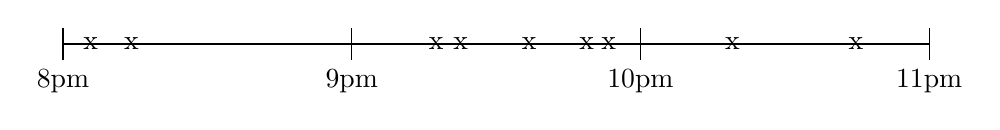
\begin{tikzpicture}

\draw (0,0) -- (11,0)
  node[pos=0.35/11]{x}
  node[pos=0.87/11]{x}
  node[pos=4.74/11]{x}
  node[pos=5.05/11]{x}
  node[pos=5.92/11]{x}
  node[pos=6.65/11]{x}
  node[pos=6.93/11]{x}
  node[pos=8.50/11]{x}
  node[pos=10.07/11]{x}
;
\node[below] at (0,-.2) {8pm};
\draw (0,-.2) -- (0,.2);
\node[below] at (11/3,-.2) {9pm};
\draw (11/3,-.2) -- (11/3,.2);
\node[below] at (22/3,-.2) {10pm};
\draw (22/3,-.2) -- (22/3,.2);
\node[below] at (11,-.2) {11pm};
\draw (11,-.2) -- (11,.2);


\end{tikzpicture}
\end{center}

Let the random variable $Y$ be the number of tweets from
the celebrity in some time interval.
When we say that the number of tweets in a time interval $t$ follows
a Poisson distribution with mean $\lambda t$, we write
\[
  Y \sim \text{Poisson($\lambda t$)}
\]
If $t$ is one hour, then we can write
\[
  Y \sim \text{Poisson($\lambda = 3$)}
\]
Stating that the number of tweets follows a Poisson distribution
implies that the time between tweets follows an Exponential
distribution (and vice versa). Let the random variable $X$ be
the time between tweets. Then
\[
  Y \sim \text{Poisson($\lambda t$)} \Longleftrightarrow X \sim \text{Exp($\lambda$)}
\]
Yes, it is the same $\lambda$ in each distribution.
The average number of tweets is $\lambda=3$ per hour. The average
time between tweets is $1/\lambda = 1/3$ hour (or 20 minutes).
Recall that for the Exponential distribution
\[
  E(X) = \frac{1}{\lambda} = \frac{1~\text{hour}}{3~\text{tweets}} = 20 ~\text{minutes per tweet on average}
\]

Questions.
\begin{enumerate}
\item What is the probability that the celebrity sends out five or
  more tweets in one hour?
\item What is the probability that the celebrity sends out
  no tweets between 9pm and 11pm?
\end{enumerate}

\section{Queueing Models}

\section{Stochastic Dynamic Programming}

\section{Probabilistic Inventory Models}

\section{Exercises}

\begin{enumerate}
  
\subsubsection*{Modeling with Probability Distributions.}

% this problem is OK
% geometric distribution
\item \emph{Searching for an item.} Albert has \num{1176} Pok\'{e}mon
  cards in total.  Pok\'{e}mon EX is a special type of card, and
  Albert has 39 EX-type cards.  He is looking for an EX-type card, but
  all of the cards are completely mixed up and stored in a shoe
  box. His mother is calling him for dinner.  What is the probability
  that Albert will have to look through no more than 25 cards before
  he finds an EX-type card?

\begin{solution}
\bs Consider finding an EX-type card to be a ``success''. Let $X$ be a
random variable that represents the number of cards that Albert has to
handle up to and including the first success. Then
\[
X \sim \text{Geometric}(p=\frac{39}{1176})
\]
and
\[
P(X \leq 25) = 1 - (1 - p)^{25} \approx 0.57.
\]
\end{solution}

% this problem is OK
% Binomial, odds, probabilities
\item \emph{Playing Pok\`{e}mon.} Albert is playing
  Pok\'{e}mon cards with his friend. It's Albert's turn, and he
  decides to use Marowak. The card says the following.
\begin{quote}
\emph{Flip a coin four times. The amount of damage done to your opponent's
Pok\'{e}mon is the number of heads times 40.}
\end{quote}
What are the odds that Marowak will do at least 120 damage to the
opponent? One approach to answer this question is to use the Binomial
distribution to compute the probability of doing at least 120 damage
and then convert from probability to odds. You can take another
approach if you prefer. In any case, assume that the coin is fair,
i.e.\ the probability of getting heads on any particular toss is 1/2.

\begin{solution}
\bs
In order to do at least 120 damage, we need either three or four heads
out of the four coin tosses. Let $X$ represent the number of heads obtained
in four tosses of a fair coin. Then $X \sim \text{Binomial}(p=1/2,n=4)$.
\begin{align*}
P(X=3) + P(X=4) &= {4 \choose 3} p^3 (1-p)^1 + {4 \choose 4} p^4 (1-p)^0 \\
&= \frac{1}{4} + \frac{1}{16} \\
&= \frac{5}{16}
\end{align*}
The odds are
\[
\frac{p}{1-p} = \frac{\frac{5}{16}}{1-\frac{5}{16}} = \frac{5}{11}
\]
or 5 to 11.
\end{solution}

% this problem needs to be re-written
% binomial distribution
\item \emph{System reliability.} 
A power utility can supply electricity to a city
from $n$ different power plants. Each power plant fails with
probability $p$, independent of the others.
\begin{enumerate}
\item Suppose that any one plant can produce enough electricity to
supply the entire city. What is the probability that the city will
experience a black-out? \label{ex:p1}
\item Suppose that two power plants are necessary to keep the city
from a black-out. Find the probability that the city will
experience a black-out. 
\label{ex:p2}
\end{enumerate}

\begin{solution}
\bs
For part~\ref{ex:p1}, all $n$ plants must fail for the city to
have a black-out. Since failures are independent, the probability
of a black-out is $p^n$.

For part~\ref{ex:p2}, let $X$ be the number of failed plants. $X$
has a Binomial distribution with parameters $n$ and $p$. The probability
of a black-out is
\begin{align*}
  P(X \geq n-1) &= \sum_{i=n-1}^n {n \choose i} p^i (1-p)^{n-i} \\
                &= {n \choose n-1} p^{n-1} (1-p)^{n-(n-1)} + {n \choose n} p^n (1-p)^{n-n} \\
                &= np^{n-1}(1-p) + p^n \\
                &= np^{n-1} - np^{n-1}p + p^n\\
                &= np^{n-1} - np^n + p^n\\
                &= np^{n-1} + (1-n)p^n
\end{align*}
\end{solution}

% this problem is OK
% exponential distribution
\item \emph{Evaluating a warranty.}
  A manufacturer of automotive batteries offers a one-year
  warranty. If the battery fails for any reason during the warranty
  period, it is replaced for free. The time to failure is distributed
  Exponential with rate $\lambda=.125$ failures per year.
\begin{enumerate}
\item What proportion of batteries fail within the warranty period?
\item The cost to manufacture a battery is \$50, and the profit
per battery is \$25. What is the effect of the warranty replacement
policy on profit? \label{ex:profit}
\end{enumerate}

\begin{solution}
  \bs The question is asking for the theoretical proportion of
  batteries that fail within one year. Since all batteries have the
  same probability of failure, this proportion is equal to the
  probability that a single battery will fail within one year. Let $X$
  be a random variable that represents the time to failure.
\[ P(X<1) = 1-e^{-\lambda t} = 1 - e^{-.125} = 0.118 \]
Now, imagine that the manufacturer has, over time,
  sold many batteries and has kept data on how many batteries failed
  within one year. The empirical proportion is simply the number
  of batteries that failed divided by the number of batteries sold.
  The Law of Large Numbers tells us that when the number of batteries
  sold is large, the empirical proportion will be approximately
  equal to the theoretical proportion.

Taking the warranty into account, the average profit per battery is
\[ \$25 - 0.118\times \$50 = \$19.10 \]
So, the (average) effect of the warranty on profit is -\$5.90.
\end{solution}

% memoryless property of the Exponential distribution this problem is
% from Ross. It's a thought experiment. The actual numbers don't
% matter as long as the rates are the same. Can we find a different
% scenario that illustrates the same idea: the memoryless property
\item \emph{Memoryless property of the Exponential distribution.}
  There are two clerks at the local post office. You enter the post
  office to find that both clerks are busy (i.e. each clerk is serving
  a customer), but that no one is in line.  So, you are first in line
  and you are to be served by the first available clerk. Customers
  depart the post office as soon as they are finished being served by
  a clerk. If the service time distribution for each clerk is
  Exponential with rate $\lambda$, what is the probability that you
  are the last of the three customers to depart the post office?

\begin{solution}
\bs
By the memoryless property of the Exponential distribution, the
remaining time for each customer currently being served is identical.
In particular, if we let $Y$ be the remaining time of a customer, then
the distribution of remaining time is
\[ P(Y \leq y) = 1 - e^{-\lambda y} \] Since the two customers have
the same distribution for remaining time, the probability that
customer 1 departs before customer 2 is 1/2 (likewise for
customer 2 departing before customer 1). When you enter service, the
memoryless property still applies.  Regardless of how long the
other customer has been in service, you have the same distribution
for remaining time. So, the probability that you are the last to depart
is 1/2.
\end{solution}

% this problem has been re-written
% Poisson distribution
\item \emph{Donut giveaway.}  A professional baseball team has just
  won a game that secured them a berth in the league’s playoffs. To
  celebrate, a local donut shop will be giving away up to 200 free
  donuts during a two-hour period on the morning following the
  victory. All 200 donuts will be baked and decorated with a baseball
  theme before the giveaway starts. If there are any donuts remaining
  after the giveaway, they will be sold at a discounted price. Assume
  that customers will arrive at the giveaway according to a Poisson
  process at a mean rate of 100 customers per hour. Also, note that
  there is a limit of one donut per customer.
\begin{enumerate}
\item What is the probability that there will be donuts remaining after the giveaway? \label{ex:donuta}
\item What is the predicted number of donuts that will be remaining after the giveaway? \label{ex:donutb}
\end{enumerate}

For part~\ref{ex:donuta}, present your answer as an expression for the
probability that there will be donuts remaining. Then, use software,
such as R, to compute a numerical answer.

\begin{solution}
  \bs Given that customers arrive to the giveaway according to a
  Poisson process with a mean of 100 customers per hour, the number of
  customers that arrive during the two-hour period is Poisson
  distributed with a mean of 200. Let $N$ be the number of customers
  arriving in a two-hour period. Then
\[ N ~ \text{Poisson}(\lambda = 200) \]
For part~\ref{ex:donuta}, the probability that there will be donuts remaining after the giveaway is 
\begin{align*}
      P(N < 200) &= \sum_{n=0}^{199} \frac{\lambda^n e^{-\lambda}}{n!}\\
      &= \sum_{n=0}^{199} \frac{200^n e^{-200}}{n!}\\
      &\approx .49
\end{align*}
In R,
\begin{Verbatim}
> sum(dpois(0:199,200))
[1] 0.4905966
\end{Verbatim}  

For part~\ref{ex:donutb}, our calculations are all done in expectation
(that is to say, on average). There are 200 customers in 2 hours,
which means that 200 donuts are given away. So, on average, no donuts
are remaining.
\end{solution}

% re-written by hannah
% Poisson distribution
\item \emph{Startup expenses.}  Two friends are starting a small
  business selling ice cream. They applied for a grant and have
  received \$\num{1800} to help cover any startup expenses. The
  friends will incur expenses of \$300 randomly throughout the first
  year, and the time between payments for these expenses is
  exponential with a mean of 2 months. Determine the probability that
  the friends will run out of grant money before the end of the year.

\begin{solution}
  \bs Let $X$ be a random variable that represents the time between
  payments. The mean time between payments, that is to say the
  expected value of $X$ ($E(X)$), is two months. We know that for the
  Exponential distribution
  \[ E(X) = \frac{1}{\lambda} \] where $\lambda$ is the rate (in units
  of payments per month). So,
  \[ X \sim \text{Exp}(\lambda = 1/2~\text{payments per month}) \] If
  the time between payments is distributed Exponential with rate
  $\lambda$, then the number of payments in $t$ months is Poisson with
  mean $\lambda t$. Let $N$ be the number of payments in 12 months.
  \[ N \sim \text{Poisson}(\lambda t = \lambda \times 12 = 6) \] Now,
  the probability that the friends runs out of money is
\begin{align*}
      P(N \geq 6) &= 1 - P(N \leq 5) \\
      &= 1 - \sum_{n=0}^{5} \frac{\lambda^n e^{-\lambda}}{n!}\\
      &= 0.55
\end{align*}
You may have defined the event that the friends runs out of
money as $P(N = 6)$. In other words, that there are exactly
six payments during the first year.  This is incorrect because
we are modeling the spending activity as a Poisson process. In
other words, the (unstated) assumption is that the number of
payments is independent of the available funds.
\end{solution}

% re-written by hannah
% poisson distribution
\item \emph{Stocking a vending machine.}  A university cafeteria has a
  vending machine that is stocked with a variety of juices and
  sodas. A vending machine attendant replenishes inventory weekly so
  that there are 180 beverages in stock at the beginning of each
  week. The cafeteria is open 24 hours, 7 days a week, and it is
  expected that the beverages will be purchased according to a Poisson
  distribution with a mean of 1 hour between purchases.
\begin{enumerate}
\item What is the probability that there are no beverages remaining in
  the vending machine when the attendant arrives? \label{ex:pout}
\item On average, how many beverages will be remaining in the vending
  machine when the attendant arrives? \label{ex:qremain}
\item What is the probability that the attendant will replenish 150 or
  more beverages? \label{ex:preplenish}
\end{enumerate}

\begin{solution}
  \bs For part~\ref{ex:pout}, there will be no beverages remaining in
  the vending machine if demand for beverages is at least 180.
  Because the beverages are purchased according to a Poisson
  distribution with a mean of one hour between purchases, the rate
  $\lambda$ that beverages are purchased is 24 beverages per
  day. Therefore, the number of purchases in seven days is Poisson
  with mean $\lambda t$. Let $N$ be a random variable that represents
  the number of purchases in one week (seven days).
  \[ N \sim \text{Poisson}(\lambda = \lambda \times 7 = 168) \] 
\begin{align*}
      P(N \geq 180) &= 1 - P(N \leq 179)\\
      &= 1 - \sum_{i=0}^{179} \frac{168^i e^{-168}}{i!}\\
      &\approx 0.19
\end{align*}
In R,
\begin{Verbatim}
> 1 - sum(dpois(0:179,168))
[1] 0.1866995
\end{Verbatim}

For part~\ref{ex:qremain}, the expected number of purchases from the
vending machine each week is 168 beverages. Therefore, the expected
number of beverages remaining at the end of the week is $180-168=12$.
	
For part~\ref{ex:preplenish}, 150 or more beverages will be
replenished if 150 or more beverages are purchased before the end of
the week. The probability that 150 or more beverages are purchased
during a week is
\begin{align*}
      P(N \geq 150) &= 1 - P(N \leq 149)\\
      &= 1 - \sum_{i=0}^{149} \frac{168^i e^{-168}}{i!}\\
      &\approx 0.93
\end{align*}
In R,
\begin{Verbatim}
> 1 - sum(dpois(0:149,168))
[1] 0.9253016
\end{Verbatim}
\end{solution}

% re-written by hannah
% Poisson distribution
\item \emph{Car dealership.} A used car dealership has an 
  uncovered lot. In the city where the
  dealership is located, the number of hailstorms during the
  month of June follows a Poisson distribution with mean four.
  After a hailstorm, the number of dents in a car
  follows a Poisson distribution with a mean of five dents.
\begin{enumerate}
\item Determine the probability that there will be exactly five
  hailstorms at the dealership in June. \label{ex:storms}
\item After a hailstorm, determine the probability that a car will
  have two or more dents. \label{ex:cars}
\end{enumerate}

\begin{solution}
  \bs For part~\ref{ex:storms}, let $X$ be a random variable that
  represents the number of hailstorms in June. The number of
  hailstorms in June follows a Poisson distribution with a mean of
  four hailstorms. Therefore, $X \sim \text{Poisson}(\lambda = 4)$.
  The probability that there are exactly five hailstorms is
\[
P(X=5) = \frac{e^{-\lambda}\lambda^5}{5!} = \frac{e^{-4}4^5}{120} \approx 0.16
\]
For part~\ref{ex:cars}, the damage to a car after a hailstorm is
Poisson with a mean of five dents. Let $N$ be the number of dents in a
car after a hailstorm.
\[ N \sim \text{Poisson}(\lambda = 5) \] 

The probability that there will be two or more dents in a car after a
hailstorm is
\begin{align*}
      P(N \geq 2) &= 1 - P(N \leq 1) \\
      &= 1 - \sum_{n=0}^{1} \frac{\lambda^n e^{-\lambda}}{n!}\\
      &\approx 0.96
\end{align*}
Using R,
\begin{Verbatim}
> 1 - sum(dpois(0:1,5))
[1] 0.9595723
\end{Verbatim}
\end{solution}

% this problem is OK
% a poisson process, memory-less property of exponential distribution
\item \emph{A mining operation.} A dump truck at a mine takes ore to
  the railroad after 10 one-ton scoops have been loaded into the
  truck.  The one-ton scoops are loaded from a large diesel-powered
  shovel independently and at a mean rate of seven scoops per hour.
  The time between scoops from the shovel can be considered to follow
  an Exponential distribution.

\begin{enumerate}
\item Find the probability that the time between consecutive trips to
  the railroad will be at least one hour.
\item It takes the dump truck 18 minutes to travel to the railroad,
  unload, and return. Suppose the truck returns and finds that no
  scoop is ready to be loaded. What is the probability that the next
  scoop is ready within 5 minutes? \label{item:2}
\end{enumerate}

\begin{solution}
  \bs The time between scoop arrivals is distributed Exponential, so
  we know that the number of arrivals in a time interval is
  distributed Poisson. In particular, the number of arrivals in a
  one-hour period follows a Poisson distribution with mean
  $\lambda=7$. In order for the time between consecutive trips to the
  railroad to take at least one hour, we require that the number of
  arrivals in one hour is nine or less. Let $X$ be the number of
  (scoop) arrivals in a one hour period.
\[
P(X \leq 9) = \sum_{x=0}^9 \frac{e^{-\lambda}\lambda^x}{x!} = .83.
\]
For part \ref{item:2}, we can invoke the memoryless property of the
Exponential distribution. The remaining time until the next arrival is
disitributed Exponential with rate 7 scoops per hour, regardless of how
much time has elapsed since the last arrival. Let $Y$ be the time
until the next arrival, and don't forget to convert from minutes to
hours.
\[
P(Y \leq 5) = 1 - e^{-7\times \frac{5}{60}} = .44
\]
\end{solution}

% re-written by hannah
% normal distribution
\item \emph{Blood pressure screening.} High blood pressure is an
  underlying health condition that makes people more susceptible to
  severe illness. A company conducted blood pressure screenings to
  determine the risk its employees have for severe illness. The
  systolic blood pressures (SBP) of 220 employees were measured.  In
  the general population, SBP measurements follow a Normal distribution
  with mean $\mu=135$ and with standard deviation $\sigma=20$.  The
  company doctor has created the following guidelines for determining
  which employees are at highest risk.

\begin{tabular}{rl}
	systolic blood pressure & risk \\ \hline
	$\mu+1.5\sigma < SBP$ & very high \\
	$\mu < SPB \leq \mu+1.5\sigma$ & high \\
	$\mu-\sigma < SBP \leq \mu$ & average \\
	$SBP \leq \mu-\sigma$ & low
\end{tabular}

How many employees of this company fall into each of the four categories?

\vspace{.1in}
\begin{solution}
\bs Let $X \sim \mathcal{N}(\mu=135,~\sigma=20)$ be a random variable that represents
systolic blood pressure, and recall that $\Phi(z)$ indicates the CDF of the
standard Normal distribution.
\begin{align*}
\text{very high}&
\quad 220\times(1-P(X \leq \mu+1.5\sigma))=220\times(1-\Phi(1.5)) \approx 15 \\
\text{high}&
\quad 220\times (P(X \leq \mu+1.5\sigma)-P(X \leq \mu))=220\times(\Phi(1.5)-\Phi(0)) \approx 95 \\
\text{average}&
\quad 220\times(P(X \leq \mu)-P(X \leq \mu-\sigma))=220\times(\Phi(0)-\Phi(-1))\approx 75 \\
\text{low}&
\quad 220\times(P(X \leq \mu-\sigma))=220\times\Phi(-1) \approx 35
\end{align*}
\end{solution}

% this problem is OK
% Lognormal distribution
\item \emph{Time to failure.} The lifetimes of parts or components
  that are subjected to the environment (i.e. temperature, corrosion,
  stress, chemicals) are often modeled using a Lognormal
  distribution. Rather than being additive, the environmental factors
  that influence the time to failure are multiplicative. The Central
  Limit Theorem applies, but because the random effects are
  multiplicative on the time scale, they are additive on the log
  scale.  

  A certain component of a bridge is inspected annually to see if it
  needs to be replaced. The lifetime of the part follows a Lognormal
  distribution with parameters $\mu=1.6$ and $\sigma=0.25$.

\begin{enumerate}
\item Determine the mean time to failure for this part.
\item What is the probability that the part will last longer
than seven years?
\end{enumerate}

\begin{solution}
  \bs Let $X$ be a random variable that represents the time to failure
of a part. Then  
\[ X \sim \text{LogN}(\mu=1.6,\sigma=0.25). \]
The mean time to failure is
\[ e^{\mu + \sigma^2/2} \approx 5.1~\text{years.} \]

We wish to find $P(X > 7)$. Taking logarithms and standardizing,
\begin{align*}
      P(X > 7) &= P(\ln(X) > \ln(7)) \\
      &= P\left(Z > \frac{\ln(7)-1.6}{0.25}\right) \\
      &= P(Z > 1.38) \\
      &= 1-P(Z \leq 1.38) \\
      &= 0.084
\end{align*}

\end{solution}


\subsubsection*{Stochastic Processes}

\subsubsection*{Queueing Models}

% this problem is ok.
\item \emph{Performance metrics for a queueing system.} Consider a
  single server queueing system with FIFO queue discipline.  For the
  particular day that this system was in operation, the arrival times
  and the service times of the first six customers were
  (0,3,7,9,10,12) and (4,6,2,1,3,1), respectively. Arrival times and
  service times are in minutes.  Compute the average waiting time and
  the average number of customers in the queue for the first six
  customers. It will help to construct a diagram of number in
  system versus time.

\begin{solution}
\bs
    
\pgfplotsset{compat=1.12}
\begin{center}
  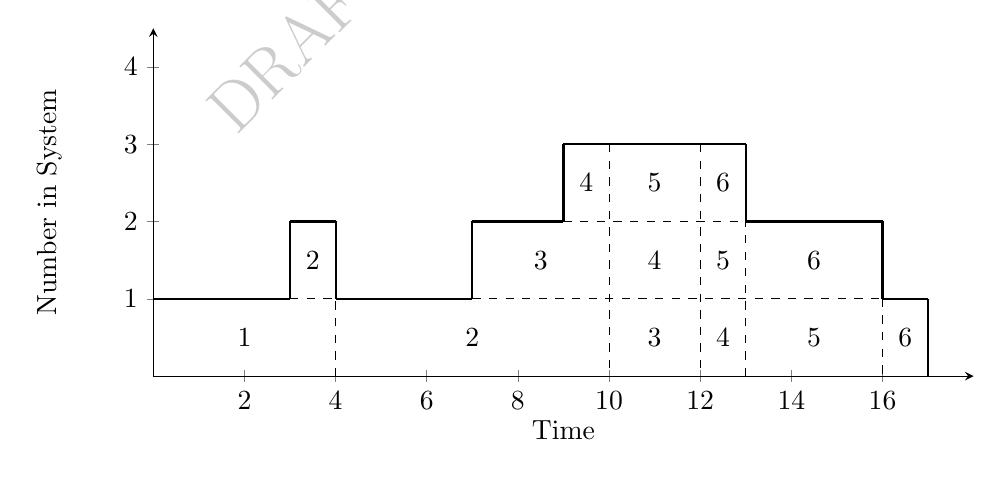
\begin{tikzpicture}[scale=1.0]
    \begin{axis}[clip=false,
      width=12cm, height=6cm,
    axis x line=middle,
    axis y line=middle,
    ymin=0, ymax=4.5,
    ytick={0,1,2,3,4},
    yticklabels={0,1,2,3,4},
    xmin=0, xmax=18,
    xtick={2,4,6,8,10,12,14,16},
    xticklabels={2,4,6,8,10,12,14,16},
    x label style={at={(axis description cs:0.5,-0.1)},anchor=north},
    y label style={at={(axis description cs:-0.1,.5)},rotate=90,anchor=south},
    xlabel=Time,
    ylabel=Number in System,
    ]
    \addplot[mark=none, style=thick] coordinates { (0, 1) (3, 1) };
    \addplot[mark=none, style=thick] coordinates { (3, 1) (3, 2) };
    \addplot[mark=none, style=thick] coordinates { (3, 2) (4, 2) };
    \addplot[mark=none, style=thick] coordinates { (4, 1) (4, 2) };
    \addplot[mark=none, style=thick] coordinates { (4, 1) (7, 1) };
    \addplot[mark=none, style=thick] coordinates { (7, 1) (7, 2) };
    \addplot[mark=none, style=thick] coordinates { (7, 2) (9, 2) };
    \addplot[mark=none, style=thick] coordinates { (9, 2) (9, 3) };
    \addplot[mark=none, style=thick] coordinates { (9, 3) (13,3) };
    \addplot[mark=none, style=thick] coordinates { (13, 3) (13,2) };
    \addplot[mark=none, style=thick] coordinates { (13,2) (16,2) };
    \addplot[mark=none, style=thick] coordinates { (16,2) (16,1) };
    \addplot[mark=none, style=thick] coordinates { (16,1) (17,1) };
    \addplot[mark=none, style=thick] coordinates { (17,1) (17,0) };

    \addplot[mark=none,dashed] coordinates { (3,1) (4,1) };
    \addplot[mark=none,dashed] coordinates { (7,1) (16,1) };
    \addplot[mark=none,dashed] coordinates { (9,2) (13,2) };
    \addplot[mark=none,dashed] coordinates { (10,3) (10,0) };
    \addplot[mark=none,dashed] coordinates { (12,3) (12,0) };
    \addplot[mark=none,dashed] coordinates { (16,1) (16,0) };
    \addplot[mark=none,dashed] coordinates { (4,0) (4,1) };
    \addplot[mark=none,dashed] coordinates { (13,0) (13,2) };

    \node at (2,.5) {1};
    \node at (3.5,1.5) {2};
    \node at (8.5,1.5) {3};
    \node at (9.5,2.5) {4};
    \node at (7,.5) {2};
    \node at (11,.5) {3};
    \node at (11,1.5) {4};
    \node at (11,2.5) {5};
    \node at (12.5,.5) {4};
    \node at (12.5,1.5) {5};
    \node at (12.5,2.5) {6};
    \node at (16.5,.5) {6};
    \node at (14.5,.5) {5};
    \node at (14.5,1.5) {6};

  \end{axis}
\end{tikzpicture}
\end{center}

First note that the problem description does \emph{not} tell us that
the times between arrivals and/or the service times are exponentially
distributed. So it is not an $M/M/1$ system.
The total delay of all six customers is $0+1+3+3+3+4=14$. The average
waiting time in the queue is the total delay divided by the number
of customers.
\[ W_q = \frac{14}{6} = 2.3333~\text{min} \]
To compute the average number in the queue, weight the time in queue
by the number of customers. In other words, compute the area under the
curve but above one, and then divide by the total time.
\[ L_q = \frac{14}{17} \]

\end{solution}

% this problem needs to be re-written.
\item \emph{Justification for a capital expense.}
Cars arrive at the Lincoln Tunnel toll gate according to a Poisson
process with an average rate of 90 cars per hour. The time for passing
the gate is exponential with mean 38 seconds.  Drivers complain of
the long waiting time, and authorities are willing to reduce the
average passing time to 30 seconds by installing automatic toll
collecting devices, provided two conditions are satisfied: 1) the
average number of waiting cars in the present system exceeds 5 and
2) the percentage of the gate idle time with the new device
installed does not exceed 10\%. Can the new device be justified?

\begin{solution}
	\bs
	Cars arrive at the rate
	\[ \lambda = 90~\text{cars per hour} \times 1/3600 =
	1~\text{car}/40~\text{seconds} \]
	We know that $\mu=1/38$
	for the current system and $\mu_{\text{new}}=1/30$ for the new
	system.
	Condition 1 states that the average number of waiting
	cars in the current system must exceed 5.
	\[ L_s = \frac{\lambda}{\mu-\lambda} = \frac{1/40}{1/38-1/40} = 19 \]
	You may have also computed
	\[ L_q = \frac{\lambda^2}{\mu(\mu-\lambda)} =
	\frac{(1/40)^2}{(1/38)(1/38 - 1/40)} = 18.05 \]
	Either way, the first condition is satisfied. The second condition
	states that the percentage of idle time in the new system cannot
	exceed 10\%.
	\[ p_0 = 1 - \frac{\lambda}{\mu_{\text{new}}} = 1 - \frac{1/40}{1/30} = .25 \]
	The second condition is not satisfied. There is no justification
	for the new toll gate device.
\end{solution}

% this problem needs to be re-written
\item \emph{Comparing system configurations.}
  Pete's Market is a small local grocery store with one checkout counter.
  Shoppers arrive at the checkout lane according to a Poisson process,
  with an arrival rate of 15 customers per hour. The checkout service times
  are distributed Exponential with a service rate of 20 customers per hour.
  The manager is considering two options for improving service.
  \begin{compactenum}
    \item Hire a second person to bag groceries while the cashier is scanning
      and collecting money from the customer. With this improved single-server
      operation, the service rate would be increased to 30 customers per hour.
    \item Hire a second person to operate a second checkout counter. The
      two-server operation would have a service rate of 20 customers per
      hour for each server.
  \end{compactenum}
  Determine the improvements that would result, consider the
  relative cost of each option, and make a recommendation to the manager.

\begin{solution}
\bs Let's look at the average number in the queue $L_Q$ and the
average time in queue $W_Q$ as metrics to judge improvement in
system performance. Because the interarrival times and the service
times are exponentially distributed, we can use the results from
section 11.2. Before any improvements are made,
\[ L_q = \frac{\lambda^2}{\mu(\mu-\lambda)} = \frac{15^2}{20(20-15)} = 2.25~\text{cust} \]
and
\[W_q = \frac{L_q}{\lambda} = \frac{2.25}{15} = .15~\text{hour} = 9~\text{min} \]
If they add a second person to the existing single checkout
\[ L_q = \frac{\lambda^2}{\mu(\mu-\lambda)} = \frac{15^2}{30(30-15)} = 0.5~\text{cust} \]
and
\[W_q = \frac{L_q}{\lambda} = \frac{0.5}{15} = 0.0333~\text{hour} = 2~\text{min} \]
and if they add a completely separate second checkout then we
need to use the formulas from section 11.3 for a two-server operation. First,
\[ P_0 = \frac{1}{\sum_{n=0}^{k-1}\frac{\left(\lambda/\mu\right)^n}{n!} + \frac{\left(\lambda/\mu\right)^k}{k!}\left(\frac{k\mu}{k\mu-\lambda}\right)} \]
where $k=2$ servers. Then
\[ L_q = \frac{\left(\lambda/\mu\right)^k\lambda\mu}{(k-1)!(k\mu-\lambda)^2}P_0 \]
and
\[W_q = \frac{L_q}{\lambda}  \]
Plugging values, I got $P_0=0.4545$, $L_q=0.123$, and $W_q=0.0082$ hours or 0.5 minutes.
Considering the relative improvement and the cost
of adding a second checkout, I would recommend option a). That is, to
add a second person to the existing checkout. The average number in
queue and the average time in queue appear to be acceptable for a
grocery store.
\end{solution}


\subsubsection*{Stochastic Dynamic Programming}

\subsubsection*{Probabilistic Inventory Models}

% the context of this problem needs to be re-written
% it is problem 27 ch 10 of IMS
\item A perishable dairy product is ordered daily at a 
  particular supermarket. The product costs
  \$1.19 per unit and sells for \$1.65 per unit. If units are unsold at
  the end of the day, the supplier takes them back at a rebate of
  \$1 per unit. Assume that daily demand is approximately normally
  distributed with $\mu = 150$ and $\sigma = 30$. 

\begin{enumerate}
\item What is your recommended daily order quantity for the
  supermarket?
\item What is the probability that the supermarket will sell all the
  units it orders?
\item In problems such as these, why would the supplier offer a rebate
  as high as \$1? For example, why not offer a nominal rebate of, say,
  25 cents per unit? What happens to the supermarket order quantity as
  the rebate is reduced? \label{rebate}
\end{enumerate}

\begin{solution}
\bs Let $D$ be the daily demand for the item. We know that
$D \sim \mathcal{N}\left(\mu=150,~\sigma=30\right)$. The penalty
for ordering too few items is $c_u=.46$ and the penalty for
ordering too many items is $c_o=.19$. We want to find the
order quantity $Q^{\ast}$ such that
\[ P\left(D \leq Q^{\ast}\right) < \frac{c_u}{c_u+c_o} = \frac{.46}{.65} = 0.708 \]
Standardizing,
\[ P\left(z \leq \frac{Q^{\ast}-150}{30}\right) = 0.708 \]
implies that
\begin{align*}
\frac{Q^{\ast}-150}{30} &= 0.55 \\
Q^{\ast} &= 150 + 0.55(30)\\
Q^{\ast} &= 166.5
\end{align*}
The supermarket should order 166 (or 167) units.  
For part b) the probability that all units will sell is
\begin{align*}
  P\left(D \geq 166 \right) &= 1 - P\left(D \leq 166 \right)\\
                            &= 1 - P\left( z \leq \frac{166-150}{30} \right) \\
                            &= 1 - P\left( z \leq .5333\right)\\
                            &= 1 - .70 \\
                            &= 0.30
\end{align*}

Regarding part~\ref{rebate}, if the rebate is \$.25 then the cost of being
under--stocked $c_u=0.46$ is less than the cost of being over--stocked
$c_o=0.94$. In this case the supermarket will order fewer items. Let's
see what happens to the supplier's revenue when the rebate is \$.25.
We want the order quantity $Q^{\ast}$ such that
\begin{align*}
  P\left(D \leq Q^{\ast}\right) = \frac{.46}{1.4} &= .329 \\
  P\left(z \leq \frac{Q^{\ast}-150}{30}\right) &= .329
\end{align*}
which implies that
\begin{align*}
  \frac{Q^{\ast}- 150}{30} &= -0.44\\
  Q^{\ast} &= 150 - 0.44(30) = 136.8
\end{align*}
or about 137 units. The expected revenue to the supplier when
$Q=166$ is
\[ 166(\$1.19) - 16(\$1.00) = \$181.54, \]
and the expected revenue when $Q=137$ is
\[ 137(\$1.19) = \$163.03. \]
As the rebate is reduced the supermarket will order fewer
items. A related question is ``What is the rebate that will
maximize the supplier's revenue?''.
\end{solution}



\end{enumerate}

\chapter{Decision Problems}

\section{Games Against Nature}


% also we need a section on using backward induction to solve
% decisions over time. relate it to DP.

\section{Games Against an Opponent}

% this will be the last portion of this section, where we bring together
% several concepts. Need to re-write this section: change the context
% of the problem and explain the methodology.
\emph{Nature as an adversary: a two-person zero-sum game.}
Merrill has a concession stand at Target Field for the sale of
sunglasses and umbrellas. This entrepreneur likes to make sales
regardless of the weather.  When it rains can sell about 500
umbrellas.  On a sunny day he can sell about 100 umbrellas and about
1000 sunglasses. Umbrellas cost him 50 cents and sell for \$1.
Sunglasses cost him 20 cents each and sell for 50 cents. Merrill is
willing to invest \$250 in the concession stand business.  All unsold
items represent a loss; there is no salvage value. 

Formulate Merrill's problem as a two-person zero--sum game. Merrill is
the row player and Nature is the column player. Merrill's strategy set
is \{buy inventory for rain, buy inventory for sun\}. Nature's strategy
set is \{rain, sun\}. The payoff entries represent the profit/loss.
Find an equilibrium strategy for Merrill. That is
to say, Merrill treats Nature as a strategic opponent and wants to
find an optimal inventory strategy that will yield a maximum expected
profit \emph{regardless} of the weather.

Would Merrill necessarily need to invest all \$250 into buying inventory
exclusively for rain or sun? In other words, does it seem possible that
Merrill could truly mix his two pure strategies and invest a portion
of the \$250 into each? The game is

\begingroup
\setlength{\tabcolsep}{9pt}
\renewcommand*{\arraystretch}{2}
\begin{tabularx}{4in}{YYYY}
& & \multicolumn{2}{c}{Nature} \\
& & Rain & Sun \\ \cline{3-4}
\multirow{2}{.5in}{Merrill} & \gtcol{Rain} & \gtcol{250} & \gtcol{-150} \\ \cline{3-4}
& \gtcol{Sun} & \gtcol{-150} & \gtcol{350} \\ \cline{3-4}
\end{tabularx}
\endgroup
\vspace{.1in}

The best strategy for Merrill is to mix buying for rain and buying
for sun in the ratio 5 to 4. These are the odds. To compute 
Merrill's expected profit (i.e. the value of the game) we use
Merrill's  equilibrium strategy against either of Nature's
pure strategies. Here is the payoff for Merrill against
Nature's strategy of Rain.

\[ \frac{5 \times (250) + 4 \times (-150)}{9} = \$72.22 \]

Merrill could play the odds and choose a pure strategy, but 
note that in this game it is possible for Merrill to physically
mix the strategies. He could invest 5/9 of his \$250 in
rainy--day inventory and invest 4/9 in sunny--day inventory.
So he buys
\[ \frac{5}{9} \left(500 \times .50\right) + \frac{4}{9} \left(100 \times .50\right) = \$161.11 \]
worth of umbrellas and
\[ \frac{4}{9} \left(1000 \times .20\right) = \$88.89 \]
worth of sunglasses so that he enjoys a steady profit of \$72.22.

\section{Utility Theory}
The payoffs in the decision problems that we have discussed have been
either monetary values or ``utilities''. So far, we haven't said much
about them.  In this section, we provide a bit more detail about the
payoff values in a decision problem.  The purpose of utility theory is
to have a convenient way to represent personal preferences over
outcomes, and by \emph{convenient} we mean numerical~\cite{luce:1957},
\cite{peterson:2009},\cite{resnik:1987}. Why is utility
important? How can utility for outcomes be more useful than simply
stating our preferences?

\begin{quote} % need to find the source ... luce and raiffa i think
Utilities are more
useful than a list of preferences for the same reason that Arabic
numerals are more useful than Roman numerals; they are better at
facilitating the transfer of information. 
\end{quote} 

It is important to note that we are not trying to explain why a
decision-maker has certain preferences over outcomes. We are just
trying to represent the preferences numerically. It turns out that
utilities are measured on an interval scale, as opposed to a ratio
scale. We cannot add, subtract, multiply, or divide utilities as we do
with measurements such as length, weight and speed, and we cannot
compare the utilities among different persons (unless they have the
same utility function).  Nevertheless, utilities capture attitudes
toward risk and utility theory is fundamental to understanding
decision problems.
\vspace{.2in} 

\begin{wrapfigure}{r}{.33\textwidth}
\centering
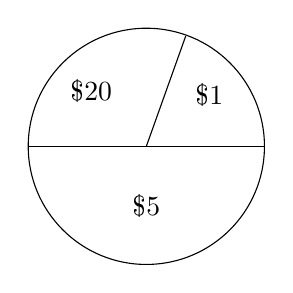
\begin{tikzpicture}
\draw (-1.5,0) -- (1.5,0);
\draw (0,0) -- (.5,1.4);
\draw (0,0) circle (1.5cm);
\draw (0,-.75) node {\$5};
\draw (-.7,.7) node {\$20};
\draw (.8,.65) node {\$1};
\end{tikzpicture}
\end{wrapfigure}

Sometimes taking a simple expected value makes sense.  Consider a
gamble in which one of three outcomes will occur. The outcomes are
worth \$1, \$5, and \$20 and the probabilities of the outcomes are .2,
.5, and .3, respectively. For example, a wheel is spun and the
probability of winning an amount corresponds to the area on the wheel.
The expected monetary value (EMV) of the gamble is
\[ \$1 \times .2 + \$5 \times .5 + \$20 \times .3 = \$8.70 \]

However, there exist situations where EMV is not an appropriate
indicator of ``fair value''. Consider another gamble in which a fair
coin is tossed until the first head appears. The gambler receives
$\$2^n$ where $n$ is the number of the tosses required until the first
instance of heads appears. So there will be $n-1$ tails followed by
heads. The probability of the first instance of heads occurring on
toss $n$ is $(1/2)^n$ and the EMV of the gamble is
\[
  2\left(\frac{1}{2}\right) + 4\left(\frac{1}{4}\right) + 8\left(\frac{1}{8}\right) +
  16\left(\frac{1}{16}\right) + \ldots = \infty.
\]
Few people (perhaps no one) would pay any amount to participate in the
gamble.  This is the St. Petersburg paradox stated by Bernoulli. To
resolve the paradox, he said that the monetary value is not as
important as the ``intrinsic worth'' of the money. For many people, an
increase in the amount of money has increasing worth, but at a
decreasing rate. Given an amount of money $m$, the logarithmic
function captures the basic relationship between $m$ and its
``intrinsic worth'' (see Figure~\vref{fig:diminishing}).

\begin{figure}
\centering
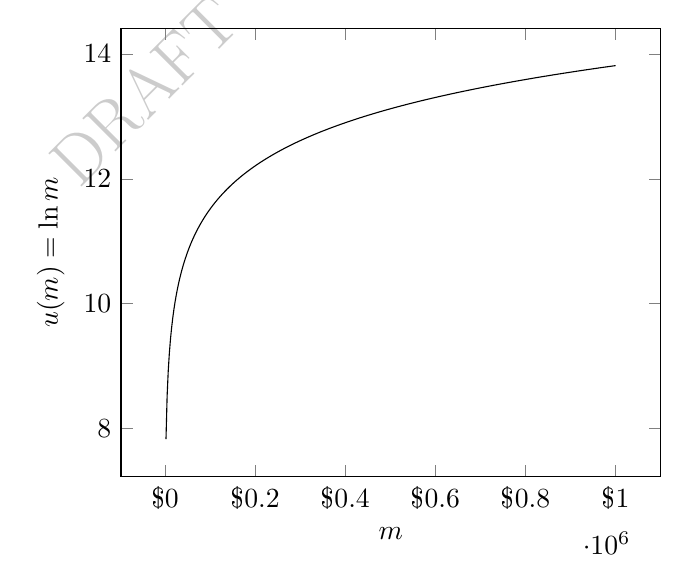
\begin{tikzpicture}
\begin{axis}[
    xlabel={$m$},
    ylabel={$u(m) = \ln m$},
    xticklabel={\$$\pgfmathprintnumber{\tick}$},
    %title={}
  ]
  \addplot[domain=0:1000000,samples=400] {ln(x)};
\end{axis}
\end{tikzpicture}
\caption{The diminishing rate of the value of money.}
\label{fig:diminishing}
\end{figure}

However, there are many functions with this basic shape and they
differ from person to person. How can the value (or utility) of money
be specified for an individual? Also, expected value is commonly
associated with value over the long run. What about a one-time
gamble? Von Neumann and Morgenstern (VnM~\cite{vonneumann:1953})
showed how to construst a utility that
represents a decision-maker's preferences (numerically) among gambles. Note that if
we were only concerned with choices among basic (certain) alternatives
then the decision-maker would simply rank the alternatives in an
ordinal manner. But we are concerned with decision-making under
risk. When we allow gambles, and ask a person to express preferences
over pairs of gambles (where the gambles are over basic alternatives)
then VnM showed how to associate utilities to the basic alternatives
in such a way that 
\begin{inparaenum}[1)] 
\item the utility for an alternative is measured by
the risk one is willing to take to receive it~\cite{savage:1972}, and
\item if decisions are made based on expected utility, then the
decision--maker is acting in agreement with her preferences.
\end{inparaenum}
Of course, the decision-maker's preferences must have some amount of
consistency. In other words, preferences must obey some rules that we
will state later.

Here is the basic idea for the construction of a utility function.
Suppose that among three different bands, Alice prefers
Smashing Pumpkins to Yo La Tengo, and she prefers Yo La Tengo to Wilco.
Now any three numbers that decrease in magnitude will capture
the ordinal preferences. But we are allowing gambles so that
we can capture Alice's attitude toward risk. We allow Alice
to choose between two alternatives 
\begin{inparaenum}[1)]
\item seeing Yo La Tengo for sure, or 
\item a gamble where she sees Smashing Pumpkins with probability
$p$ or Wilco with probability $1-p$. 
\end{inparaenum}
If $p$ is very close to one then Alice will choose the gamble. But if we
decrease $p$, then at \emph{some} point Alice will prefer the certain
alternative of seeing Yo La Tengo. We ask Alice for the value of
$p$ at which she is indifferent between the certain alternative and
the gamble. Suppose Alice indicates
$p=2/3$. Now, arbitrarily associate the value 1 with Smashing Pumpkins
and associate the value 0 with Wilco. Then it seems natural to
associate the value 2/3 with Yo La Tengo. Note that the value of Yo La
Tengo equals the expected value of the gamble.
\[ \frac{2}{3} = 1\left(\frac{2}{3}\right) +
  0\left(\frac{1}{3}\right) \] Instead of using (1, 2/3, 0) we could
use \emph{any} three numbers $a+c,~(2/3)a+c,~c$, where $a$ and
$c$ are constants and
$a>0$, and not alter the preferences (including the preference over the
certain outcome and the gamble).

Perhaps the most troublesome aspect of constructing utilities in this
way is the natural inclination to think about the utility values in
terms of ratios. You should avoid doing this.  For example, it is
\emph{not} correct to say that Alice prefers seeing Yo La Tengo to
seeing Wilco twice as much as she prefers seeing Smashing Pumpkins to
seeing Yo La Tengo. No! The number 2/3 reflects Alice's attitude
toward gambling, not her attitude toward the two intervals. A commonly
used example~\cite{luce:1957} to illustrate this fact is the
following. Suppose you like taking chances. You are
indifferent between 1) receiving \$9 for sure, or 2) participating in
a gamble that results in equal chances of receiving either \$10 or
nothing. Your utilities for the three amounts \$10, \$9 and \$0 are 1,
1/2, and 0, respectively. It's not that you have equal preferences
for going from \$0 to \$9 and going from \$9 to \$10. No. You simply
like taking chances.

Another common mistake is to say that Alice prefers Smashing Pumpkins
to Yo La Tengo because Smashing Pumpkins has higher utility. No!
Alice's preferences (and your preferences) among basic alternatives
and lotteries come first. A decision-maker knows her preferences. The
point is that if Alice can state her preferences, then we can
construct a numerical characterization of them. That is to say, we can
associate a value (i.e. a number) to something that is inherently
non-numeric.  The expected utility theorem is a representation
theorem.

\label{rules-of-consistency}
Now for the rules of consistency. Let $L(p,x,y)$ represent a gamble
(also called a lottery) in which you receive outcome $x$ with
probability $p$ or you receive outcome $y$ with probability
$(1-p)$. Also, let $x \succ y$ indicate that outcome $x$ is preferred
to outcome $y$, and let $x \sim y$ indicate indifference between the
outcomes $x$ and $y$. A decision-maker's preferences must satisfy the
following rules. (Note that the rules don't seem too objectionable).
\begin{enumerate}
\item $x \succ y$ or $y \succ x$ or $x \sim y$. (completeness)
\item if $x \succ y$ and $y \succ z$ then $x \succ z$. (transitivity)
\item $L\left(p,L(q,x,y),L(r,x,y)\right) \sim L(s,x,y)$ where $s=pq+(1-p)r$. (no fun in gambling)
\item given $x \succ y \succ z$, there is some lottery $L(p,x,z) \sim y$. (continuity)
\item if two lotteries are identical except for the first prize, then the
  lottery with the better first prize is preferred. (better prizes condition)
\item if two lotteries have the same alternatives as prizes, then the
  lottery that assigns higher probability of winning the best prize is
  preferred. (better chances condition)
\end{enumerate}
If you can state your preferences according to the above rules,
then an \emph{interval} utility function $u()$ can be constructed
in such a way that
\begin{enumerate}[i)]
\item $u(x) \succ u(y) \iff x \succ y$ \label{eu1}
\item $u(x) = u(y) \iff x \sim y$ \label{eu2}
\item $u\left(L(p,x,y)\right) = pu(x) + (1-p)u(y)$ 
(expected utility property) \label{eu3}
\item if $u'()$ is a positive linear transformation of $u()$ then
  $u'()$ also satisfies \ref{eu1}, \ref{eu2}, and \ref{eu3}. \label{eu4}
\end{enumerate}
Items \ref{eu1} through \ref{eu4} constitute the Expected Utility
Theorem.  When working through exercises, perhaps the most useful item is
item \ref{eu3}, the expected utility property. It states that the utility
of a lottery is equal to its expected utility. Do \emph{not} confuse
expected utility with the utility of the expected value, which is not
of interest.

\emph{Retirement and risk}.  This example is inspired from the
discussion on utility in Chernoff and Moses~\cite{chernoff:1959}.
Alice currently has \$\num{400000} in her individual retirement
account (IRA). Of course, it is always better to have more money for
retirement, but Alice is not super-greedy; she wants to have enough
money to pay bills and take a few backpacking trips each year.  Her
utility for an amount of money $m$ in the range \$0 to \$1 million is
given by the following function and is shown in
Figure~\vref{fig:retirement}.

\[
u(m) = \frac{10}{1+e^{-(\frac{m}{\num{500000}}-5)}}
\]

\begin{figure}
\centering
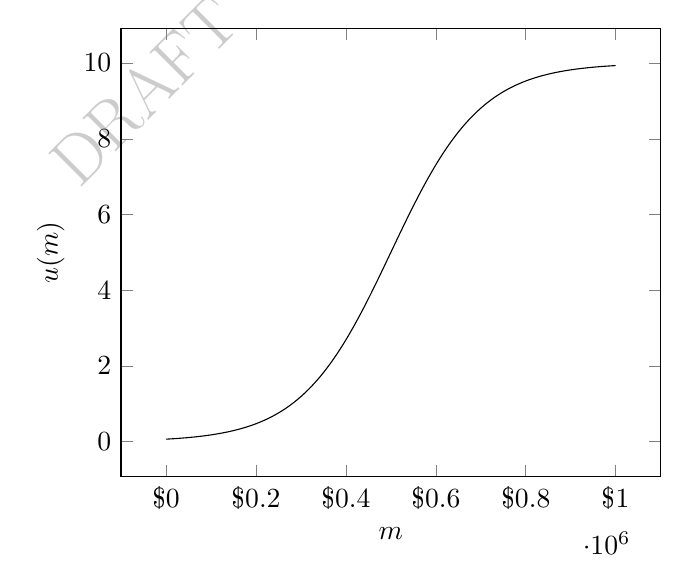
\begin{tikzpicture}
\begin{axis}[
    xlabel={$m$},
    ylabel={$u(m)$},
    xticklabel={\$$\pgfmathprintnumber{\tick}$},
    %title={Utility function for the retirement funds}
  ]
  %\addplot[domain=0:1000000,samples=1000] {10 / (1 + exp(-(x/500000 - 5)))};
  % tikz was plottting the function incorrectly, so for now i am resorting
  % to coordinates.
  \addplot[color=black,mark=none]
  coordinates {
(0,0.0669)(1000,0.0676)(2000,0.0683)(3000,0.069)(4000,0.0696)
(5000,0.0703)(6000,0.071)(7000,0.0717)(8000,0.0725)(9000,0.0732)
(10000,0.0739)(11000,0.0747)(12000,0.0754)(13000,0.0761)(14000,0.0769)
(15000,0.0777)(16000,0.0785)(17000,0.0792)(18000,0.08)(19000,0.0808)
(20000,0.0816)(21000,0.0824)(22000,0.0833)(23000,0.0841)(24000,0.0849)
(25000,0.0858)(26000,0.0866)(27000,0.0875)(28000,0.0884)(29000,0.0892)
(30000,0.0901)(31000,0.091)(32000,0.0919)(33000,0.0929)(34000,0.0938)
(35000,0.0947)(36000,0.0957)(37000,0.0966)(38000,0.0976)(39000,0.0985)
(40000,0.0995)(41000,0.1005)(42000,0.1015)(43000,0.1025)(44000,0.1035)
(45000,0.1046)(46000,0.1056)(47000,0.1067)(48000,0.1077)(49000,0.1088)
(50000,0.1099)(51000,0.111)(52000,0.1121)(53000,0.1132)(54000,0.1143)
(55000,0.1154)(56000,0.1166)(57000,0.1177)(58000,0.1189)(59000,0.1201)
(60000,0.1213)(61000,0.1225)(62000,0.1237)(63000,0.1249)(64000,0.1262)
(65000,0.1274)(66000,0.1287)(67000,0.13)(68000,0.1313)(69000,0.1326)
(70000,0.1339)(71000,0.1352)(72000,0.1365)(73000,0.1379)(74000,0.1393)
(75000,0.1406)(76000,0.142)(77000,0.1434)(78000,0.1449)(79000,0.1463)
(80000,0.1477)(81000,0.1492)(82000,0.1507)(83000,0.1522)(84000,0.1537)
(85000,0.1552)(86000,0.1567)(87000,0.1583)(88000,0.1598)(89000,0.1614)
(90000,0.163)(91000,0.1646)(92000,0.1663)(93000,0.1679)(94000,0.1696)
(95000,0.1712)(96000,0.1729)(97000,0.1746)(98000,0.1764)(99000,0.1781)
(1e+05,0.1799)(101000,0.1816)(102000,0.1834)(103000,0.1852)(104000,0.1871)
(105000,0.1889)(106000,0.1908)(107000,0.1927)(108000,0.1946)(109000,0.1965)
(110000,0.1984)(111000,0.2004)(112000,0.2023)(113000,0.2043)(114000,0.2063)
(115000,0.2084)(116000,0.2104)(117000,0.2125)(118000,0.2146)(119000,0.2167)
(120000,0.2188)(121000,0.221)(122000,0.2231)(123000,0.2253)(124000,0.2275)
(125000,0.2298)(126000,0.232)(127000,0.2343)(128000,0.2366)(129000,0.2389)
(130000,0.2413)(131000,0.2436)(132000,0.246)(133000,0.2484)(134000,0.2509)
(135000,0.2533)(136000,0.2558)(137000,0.2583)(138000,0.2608)(139000,0.2634)
(140000,0.266)(141000,0.2686)(142000,0.2712)(143000,0.2738)(144000,0.2765)
(145000,0.2792)(146000,0.282)(147000,0.2847)(148000,0.2875)(149000,0.2903)
(150000,0.2931)(151000,0.296)(152000,0.2989)(153000,0.3018)(154000,0.3047)
(155000,0.3077)(156000,0.3107)(157000,0.3137)(158000,0.3168)(159000,0.3198)
(160000,0.323)(161000,0.3261)(162000,0.3293)(163000,0.3325)(164000,0.3357)
(165000,0.339)(166000,0.3422)(167000,0.3456)(168000,0.3489)(169000,0.3523)
(170000,0.3557)(171000,0.3592)(172000,0.3626)(173000,0.3661)(174000,0.3697)
(175000,0.3733)(176000,0.3769)(177000,0.3805)(178000,0.3842)(179000,0.3879)
(180000,0.3917)(181000,0.3954)(182000,0.3993)(183000,0.4031)(184000,0.407)
(185000,0.4109)(186000,0.4149)(187000,0.4189)(188000,0.4229)(189000,0.427)
(190000,0.4311)(191000,0.4352)(192000,0.4394)(193000,0.4436)(194000,0.4479)
(195000,0.4522)(196000,0.4565)(197000,0.4609)(198000,0.4653)(199000,0.4698)
(2e+05,0.4743)(201000,0.4788)(202000,0.4834)(203000,0.488)(204000,0.4927)
(205000,0.4974)(206000,0.5021)(207000,0.5069)(208000,0.5117)(209000,0.5166)
(210000,0.5215)(211000,0.5265)(212000,0.5315)(213000,0.5366)(214000,0.5417)
(215000,0.5468)(216000,0.552)(217000,0.5572)(218000,0.5625)(219000,0.5679)
(220000,0.5732)(221000,0.5787)(222000,0.5841)(223000,0.5897)(224000,0.5952)
(225000,0.6009)(226000,0.6065)(227000,0.6123)(228000,0.618)(229000,0.6239)
(230000,0.6297)(231000,0.6357)(232000,0.6416)(233000,0.6477)(234000,0.6538)
(235000,0.6599)(236000,0.6661)(237000,0.6723)(238000,0.6786)(239000,0.685)
(240000,0.6914)(241000,0.6978)(242000,0.7044)(243000,0.7109)(244000,0.7176)
(245000,0.7243)(246000,0.731)(247000,0.7378)(248000,0.7447)(249000,0.7516)
(250000,0.7586)(251000,0.7656)(252000,0.7727)(253000,0.7799)(254000,0.7871)
(255000,0.7944)(256000,0.8017)(257000,0.8091)(258000,0.8166)(259000,0.8241)
(260000,0.8317)(261000,0.8394)(262000,0.8471)(263000,0.8549)(264000,0.8627)
(265000,0.8707)(266000,0.8786)(267000,0.8867)(268000,0.8948)(269000,0.903)
(270000,0.9112)(271000,0.9195)(272000,0.9279)(273000,0.9364)(274000,0.9449)
(275000,0.9535)(276000,0.9622)(277000,0.9709)(278000,0.9797)(279000,0.9886)
(280000,0.9975)(281000,1.0065)(282000,1.0156)(283000,1.0248)(284000,1.034)
(285000,1.0433)(286000,1.0527)(287000,1.0621)(288000,1.0717)(289000,1.0813)
(290000,1.091)(291000,1.1007)(292000,1.1106)(293000,1.1205)(294000,1.1305)
(295000,1.1405)(296000,1.1507)(297000,1.1609)(298000,1.1712)(299000,1.1816)
(3e+05,1.192)(301000,1.2026)(302000,1.2132)(303000,1.2239)(304000,1.2347)
(305000,1.2455)(306000,1.2565)(307000,1.2675)(308000,1.2786)(309000,1.2898)
(310000,1.3011)(311000,1.3124)(312000,1.3239)(313000,1.3354)(314000,1.347)
(315000,1.3587)(316000,1.3705)(317000,1.3824)(318000,1.3943)(319000,1.4064)
(320000,1.4185)(321000,1.4307)(322000,1.443)(323000,1.4554)(324000,1.4679)
(325000,1.4805)(326000,1.4931)(327000,1.5059)(328000,1.5187)(329000,1.5316)
(330000,1.5447)(331000,1.5578)(332000,1.571)(333000,1.5842)(334000,1.5976)
(335000,1.6111)(336000,1.6247)(337000,1.6383)(338000,1.652)(339000,1.6659)
(340000,1.6798)(341000,1.6938)(342000,1.708)(343000,1.7222)(344000,1.7365)
(345000,1.7509)(346000,1.7654)(347000,1.7799)(348000,1.7946)(349000,1.8094)
(350000,1.8243)(351000,1.8392)(352000,1.8543)(353000,1.8694)(354000,1.8847)
(355000,1.9)(356000,1.9155)(357000,1.931)(358000,1.9466)(359000,1.9623)
(360000,1.9782)(361000,1.9941)(362000,2.0101)(363000,2.0262)(364000,2.0424)
(365000,2.0587)(366000,2.0751)(367000,2.0916)(368000,2.1082)(369000,2.1249)
(370000,2.1417)(371000,2.1585)(372000,2.1755)(373000,2.1926)(374000,2.2097)
(375000,2.227)(376000,2.2444)(377000,2.2618)(378000,2.2794)(379000,2.297)
(380000,2.3148)(381000,2.3326)(382000,2.3505)(383000,2.3685)(384000,2.3867)
(385000,2.4049)(386000,2.4232)(387000,2.4416)(388000,2.4601)(389000,2.4787)
(390000,2.4974)(391000,2.5162)(392000,2.5351)(393000,2.554)(394000,2.5731)
(395000,2.5923)(396000,2.6115)(397000,2.6308)(398000,2.6503)(399000,2.6698)
(4e+05,2.6894)(401000,2.7091)(402000,2.7289)(403000,2.7488)(404000,2.7688)
(405000,2.7888)(406000,2.809)(407000,2.8292)(408000,2.8496)(409000,2.87)
(410000,2.8905)(411000,2.9111)(412000,2.9318)(413000,2.9525)(414000,2.9734)
(415000,2.9943)(416000,3.0153)(417000,3.0365)(418000,3.0576)(419000,3.0789)
(420000,3.1003)(421000,3.1217)(422000,3.1432)(423000,3.1648)(424000,3.1865)
(425000,3.2082)(426000,3.23)(427000,3.2519)(428000,3.2739)(429000,3.296)
(430000,3.3181)(431000,3.3403)(432000,3.3626)(433000,3.385)(434000,3.4074)
(435000,3.4299)(436000,3.4525)(437000,3.4751)(438000,3.4978)(439000,3.5206)
(440000,3.5434)(441000,3.5663)(442000,3.5893)(443000,3.6124)(444000,3.6355)
(445000,3.6586)(446000,3.6819)(447000,3.7052)(448000,3.7285)(449000,3.7519)
(450000,3.7754)(451000,3.7989)(452000,3.8225)(453000,3.8462)(454000,3.8699)
(455000,3.8936)(456000,3.9174)(457000,3.9413)(458000,3.9652)(459000,3.9891)
(460000,4.0131)(461000,4.0372)(462000,4.0613)(463000,4.0854)(464000,4.1096)
(465000,4.1338)(466000,4.1581)(467000,4.1824)(468000,4.2068)(469000,4.2311)
(470000,4.2556)(471000,4.28)(472000,4.3045)(473000,4.3291)(474000,4.3536)
(475000,4.3782)(476000,4.4029)(477000,4.4275)(478000,4.4522)(479000,4.4769)
(480000,4.5017)(481000,4.5264)(482000,4.5512)(483000,4.576)(484000,4.6009)
(485000,4.6257)(486000,4.6506)(487000,4.6755)(488000,4.7004)(489000,4.7253)
(490000,4.7502)(491000,4.7752)(492000,4.8001)(493000,4.8251)(494000,4.85)
(495000,4.875)(496000,4.9)(497000,4.925)(498000,4.95)(499000,4.975)
(5e+05,5)(501000,5.025)(502000,5.05)(503000,5.075)(504000,5.1)
(505000,5.125)(506000,5.15)(507000,5.1749)(508000,5.1999)(509000,5.2248)
(510000,5.2498)(511000,5.2747)(512000,5.2996)(513000,5.3245)(514000,5.3494)
(515000,5.3743)(516000,5.3991)(517000,5.424)(518000,5.4488)(519000,5.4736)
(520000,5.4983)(521000,5.5231)(522000,5.5478)(523000,5.5725)(524000,5.5971)
(525000,5.6218)(526000,5.6464)(527000,5.6709)(528000,5.6955)(529000,5.72)
(530000,5.7444)(531000,5.7689)(532000,5.7932)(533000,5.8176)(534000,5.8419)
(535000,5.8662)(536000,5.8904)(537000,5.9146)(538000,5.9387)(539000,5.9628)
(540000,5.9869)(541000,6.0109)(542000,6.0348)(543000,6.0587)(544000,6.0826)
(545000,6.1064)(546000,6.1301)(547000,6.1538)(548000,6.1775)(549000,6.2011)
(550000,6.2246)(551000,6.2481)(552000,6.2715)(553000,6.2948)(554000,6.3181)
(555000,6.3414)(556000,6.3645)(557000,6.3876)(558000,6.4107)(559000,6.4337)
(560000,6.4566)(561000,6.4794)(562000,6.5022)(563000,6.5249)(564000,6.5475)
(565000,6.5701)(566000,6.5926)(567000,6.615)(568000,6.6374)(569000,6.6597)
(570000,6.6819)(571000,6.704)(572000,6.7261)(573000,6.7481)(574000,6.77)
(575000,6.7918)(576000,6.8135)(577000,6.8352)(578000,6.8568)(579000,6.8783)
(580000,6.8997)(581000,6.9211)(582000,6.9424)(583000,6.9635)(584000,6.9847)
(585000,7.0057)(586000,7.0266)(587000,7.0475)(588000,7.0682)(589000,7.0889)
(590000,7.1095)(591000,7.13)(592000,7.1504)(593000,7.1708)(594000,7.191)
(595000,7.2112)(596000,7.2312)(597000,7.2512)(598000,7.2711)(599000,7.2909)
(6e+05,7.3106)(601000,7.3302)(602000,7.3497)(603000,7.3692)(604000,7.3885)
(605000,7.4077)(606000,7.4269)(607000,7.446)(608000,7.4649)(609000,7.4838)
(610000,7.5026)(611000,7.5213)(612000,7.5399)(613000,7.5584)(614000,7.5768)
(615000,7.5951)(616000,7.6133)(617000,7.6315)(618000,7.6495)(619000,7.6674)
(620000,7.6852)(621000,7.703)(622000,7.7206)(623000,7.7382)(624000,7.7556)
(625000,7.773)(626000,7.7903)(627000,7.8074)(628000,7.8245)(629000,7.8415)
(630000,7.8583)(631000,7.8751)(632000,7.8918)(633000,7.9084)(634000,7.9249)
(635000,7.9413)(636000,7.9576)(637000,7.9738)(638000,7.9899)(639000,8.0059)
(640000,8.0218)(641000,8.0377)(642000,8.0534)(643000,8.069)(644000,8.0845)
(645000,8.1)(646000,8.1153)(647000,8.1306)(648000,8.1457)(649000,8.1608)
(650000,8.1757)(651000,8.1906)(652000,8.2054)(653000,8.2201)(654000,8.2346)
(655000,8.2491)(656000,8.2635)(657000,8.2778)(658000,8.292)(659000,8.3062)
(660000,8.3202)(661000,8.3341)(662000,8.348)(663000,8.3617)(664000,8.3753)
(665000,8.3889)(666000,8.4024)(667000,8.4158)(668000,8.429)(669000,8.4422)
(670000,8.4553)(671000,8.4684)(672000,8.4813)(673000,8.4941)(674000,8.5069)
(675000,8.5195)(676000,8.5321)(677000,8.5446)(678000,8.557)(679000,8.5693)
(680000,8.5815)(681000,8.5936)(682000,8.6057)(683000,8.6176)(684000,8.6295)
(685000,8.6413)(686000,8.653)(687000,8.6646)(688000,8.6761)(689000,8.6876)
(690000,8.6989)(691000,8.7102)(692000,8.7214)(693000,8.7325)(694000,8.7435)
(695000,8.7545)(696000,8.7653)(697000,8.7761)(698000,8.7868)(699000,8.7974)
(7e+05,8.808)(701000,8.8184)(702000,8.8288)(703000,8.8391)(704000,8.8493)
(705000,8.8595)(706000,8.8695)(707000,8.8795)(708000,8.8894)(709000,8.8993)
(710000,8.909)(711000,8.9187)(712000,8.9283)(713000,8.9379)(714000,8.9473)
(715000,8.9567)(716000,8.966)(717000,8.9752)(718000,8.9844)(719000,8.9935)
(720000,9.0025)(721000,9.0114)(722000,9.0203)(723000,9.0291)(724000,9.0378)
(725000,9.0465)(726000,9.0551)(727000,9.0636)(728000,9.0721)(729000,9.0805)
(730000,9.0888)(731000,9.097)(732000,9.1052)(733000,9.1133)(734000,9.1214)
(735000,9.1293)(736000,9.1373)(737000,9.1451)(738000,9.1529)(739000,9.1606)
(740000,9.1683)(741000,9.1759)(742000,9.1834)(743000,9.1909)(744000,9.1983)
(745000,9.2056)(746000,9.2129)(747000,9.2201)(748000,9.2273)(749000,9.2344)
(750000,9.2414)(751000,9.2484)(752000,9.2553)(753000,9.2622)(754000,9.269)
(755000,9.2757)(756000,9.2824)(757000,9.2891)(758000,9.2956)(759000,9.3022)
(760000,9.3086)(761000,9.315)(762000,9.3214)(763000,9.3277)(764000,9.3339)
(765000,9.3401)(766000,9.3462)(767000,9.3523)(768000,9.3584)(769000,9.3643)
(770000,9.3703)(771000,9.3761)(772000,9.382)(773000,9.3877)(774000,9.3935)
(775000,9.3991)(776000,9.4048)(777000,9.4103)(778000,9.4159)(779000,9.4213)
(780000,9.4268)(781000,9.4321)(782000,9.4375)(783000,9.4428)(784000,9.448)
(785000,9.4532)(786000,9.4583)(787000,9.4634)(788000,9.4685)(789000,9.4735)
(790000,9.4785)(791000,9.4834)(792000,9.4883)(793000,9.4931)(794000,9.4979)
(795000,9.5026)(796000,9.5073)(797000,9.512)(798000,9.5166)(799000,9.5212)
(8e+05,9.5257)(801000,9.5302)(802000,9.5347)(803000,9.5391)(804000,9.5435)
(805000,9.5478)(806000,9.5521)(807000,9.5564)(808000,9.5606)(809000,9.5648)
(810000,9.5689)(811000,9.573)(812000,9.5771)(813000,9.5811)(814000,9.5851)
(815000,9.5891)(816000,9.593)(817000,9.5969)(818000,9.6007)(819000,9.6046)
(820000,9.6083)(821000,9.6121)(822000,9.6158)(823000,9.6195)(824000,9.6231)
(825000,9.6267)(826000,9.6303)(827000,9.6339)(828000,9.6374)(829000,9.6408)
(830000,9.6443)(831000,9.6477)(832000,9.6511)(833000,9.6544)(834000,9.6578)
(835000,9.661)(836000,9.6643)(837000,9.6675)(838000,9.6707)(839000,9.6739)
(840000,9.677)(841000,9.6802)(842000,9.6832)(843000,9.6863)(844000,9.6893)
(845000,9.6923)(846000,9.6953)(847000,9.6982)(848000,9.7011)(849000,9.704)
(850000,9.7069)(851000,9.7097)(852000,9.7125)(853000,9.7153)(854000,9.718)
(855000,9.7208)(856000,9.7235)(857000,9.7262)(858000,9.7288)(859000,9.7314)
(860000,9.734)(861000,9.7366)(862000,9.7392)(863000,9.7417)(864000,9.7442)
(865000,9.7467)(866000,9.7491)(867000,9.7516)(868000,9.754)(869000,9.7564)
(870000,9.7587)(871000,9.7611)(872000,9.7634)(873000,9.7657)(874000,9.768)
(875000,9.7702)(876000,9.7725)(877000,9.7747)(878000,9.7769)(879000,9.779)
(880000,9.7812)(881000,9.7833)(882000,9.7854)(883000,9.7875)(884000,9.7896)
(885000,9.7916)(886000,9.7937)(887000,9.7957)(888000,9.7977)(889000,9.7996)
(890000,9.8016)(891000,9.8035)(892000,9.8054)(893000,9.8073)(894000,9.8092)
(895000,9.8111)(896000,9.8129)(897000,9.8148)(898000,9.8166)(899000,9.8184)
(9e+05,9.8201)(901000,9.8219)(902000,9.8236)(903000,9.8254)(904000,9.8271)
(905000,9.8288)(906000,9.8304)(907000,9.8321)(908000,9.8337)(909000,9.8354)
(910000,9.837)(911000,9.8386)(912000,9.8402)(913000,9.8417)(914000,9.8433)
(915000,9.8448)(916000,9.8463)(917000,9.8478)(918000,9.8493)(919000,9.8508)
(920000,9.8523)(921000,9.8537)(922000,9.8551)(923000,9.8566)(924000,9.858)
(925000,9.8594)(926000,9.8607)(927000,9.8621)(928000,9.8635)(929000,9.8648)
(930000,9.8661)(931000,9.8674)(932000,9.8687)(933000,9.87)(934000,9.8713)
(935000,9.8726)(936000,9.8738)(937000,9.8751)(938000,9.8763)(939000,9.8775)
(940000,9.8787)(941000,9.8799)(942000,9.8811)(943000,9.8823)(944000,9.8834)
(945000,9.8846)(946000,9.8857)(947000,9.8868)(948000,9.8879)(949000,9.889)
(950000,9.8901)(951000,9.8912)(952000,9.8923)(953000,9.8933)(954000,9.8944)
(955000,9.8954)(956000,9.8965)(957000,9.8975)(958000,9.8985)(959000,9.8995)
(960000,9.9005)(961000,9.9015)(962000,9.9024)(963000,9.9034)(964000,9.9043)
(965000,9.9053)(966000,9.9062)(967000,9.9071)(968000,9.9081)(969000,9.909)
(970000,9.9099)(971000,9.9108)(972000,9.9116)(973000,9.9125)(974000,9.9134)
(975000,9.9142)(976000,9.9151)(977000,9.9159)(978000,9.9167)(979000,9.9176)
(980000,9.9184)(981000,9.9192)(982000,9.92)(983000,9.9208)(984000,9.9215)
(985000,9.9223)(986000,9.9231)(987000,9.9239)(988000,9.9246)(989000,9.9253)
(990000,9.9261)(991000,9.9268)(992000,9.9275)(993000,9.9283)(994000,9.929)
(995000,9.9297)(996000,9.9304)(997000,9.931)(998000,9.9317)(999000,9.9324)
(1e+06,9.9331)
  };
\end{axis}
\end{tikzpicture}
\caption{Utility function for the retirement funds.}
\label{fig:retirement}
\end{figure}

Note that her current utility is
$u(\$\num{400000})=2.69$.  Suppose that on a trip to Las Vegas, Alice
is offered a gambling opportunity for gaining \$\num{200000} or losing
\$\num{100000}. The odds are 1-to-1 for gaining and losing. If Alice wins,
she will have \$\num{600000}, but if she loses, she will have
\$\num{300000}. Alice knows about the the expected utility property:
that the utility of a lottery is equal to its expected
utility. Converting from odds to probabilities, she computes the
utility of the gamble as
\[
\frac{1}{2}u(\$\num{600000}) + \frac{1}{2}u(\$\num{300000}) = 4.25,
\]
which is higher than her current utility so she takes the gamble.

Suppose that Alice wins. She now had \$\num{600000} and her utility is
$u(\$\num{600000}) = 7.31$.  
Gaining confidence in her luck, Alice seeks and finds another
opportunity. The new gamble has odds of 1-to-2 for winning
\$\num{200000} or losing \$\num{100000}. 
The probability $p$ of winning is
\[
p = \frac{\text{odds}}{\text{odds}+1} = 
\frac{\frac{1}{2}}{\frac{1}{2} + 1} = \frac{1}{3}.
\]
Notice that the gamble is fair because
\[
\frac{1}{3}u(\$\num{200000}) - \frac{2}{3}u(\$\num{100000}) = 0.
\]
\emph{Alice's} utility for the new opportunity is
\[
\frac{1}{3}u(\$\num{800000}) + \frac{2}{3}u(\$\num{500000}) = 6.51,
\]
which is less than her current utility and so, even though
the gamble is fair, she declines.

\tikzstyle{place}=[circle,draw,minimum size=.75mm,
  inner sep=0pt,fill=black]
\begin{figure}
\centering
\begin{tikzpicture}
\begin{axis}[
    xlabel={$m$},
    ylabel={$u(m)$},
    xticklabel={\$$\pgfmathprintnumber{\tick}$},
    %title={A graphic interpretation of the gamble}
  ]
  \addplot[color=black,mark=none]
  coordinates {
(0,0.0669)(1000,0.0676)(2000,0.0683)(3000,0.069)(4000,0.0696)
(5000,0.0703)(6000,0.071)(7000,0.0717)(8000,0.0725)(9000,0.0732)
(10000,0.0739)(11000,0.0747)(12000,0.0754)(13000,0.0761)(14000,0.0769)
(15000,0.0777)(16000,0.0785)(17000,0.0792)(18000,0.08)(19000,0.0808)
(20000,0.0816)(21000,0.0824)(22000,0.0833)(23000,0.0841)(24000,0.0849)
(25000,0.0858)(26000,0.0866)(27000,0.0875)(28000,0.0884)(29000,0.0892)
(30000,0.0901)(31000,0.091)(32000,0.0919)(33000,0.0929)(34000,0.0938)
(35000,0.0947)(36000,0.0957)(37000,0.0966)(38000,0.0976)(39000,0.0985)
(40000,0.0995)(41000,0.1005)(42000,0.1015)(43000,0.1025)(44000,0.1035)
(45000,0.1046)(46000,0.1056)(47000,0.1067)(48000,0.1077)(49000,0.1088)
(50000,0.1099)(51000,0.111)(52000,0.1121)(53000,0.1132)(54000,0.1143)
(55000,0.1154)(56000,0.1166)(57000,0.1177)(58000,0.1189)(59000,0.1201)
(60000,0.1213)(61000,0.1225)(62000,0.1237)(63000,0.1249)(64000,0.1262)
(65000,0.1274)(66000,0.1287)(67000,0.13)(68000,0.1313)(69000,0.1326)
(70000,0.1339)(71000,0.1352)(72000,0.1365)(73000,0.1379)(74000,0.1393)
(75000,0.1406)(76000,0.142)(77000,0.1434)(78000,0.1449)(79000,0.1463)
(80000,0.1477)(81000,0.1492)(82000,0.1507)(83000,0.1522)(84000,0.1537)
(85000,0.1552)(86000,0.1567)(87000,0.1583)(88000,0.1598)(89000,0.1614)
(90000,0.163)(91000,0.1646)(92000,0.1663)(93000,0.1679)(94000,0.1696)
(95000,0.1712)(96000,0.1729)(97000,0.1746)(98000,0.1764)(99000,0.1781)
(1e+05,0.1799)(101000,0.1816)(102000,0.1834)(103000,0.1852)(104000,0.1871)
(105000,0.1889)(106000,0.1908)(107000,0.1927)(108000,0.1946)(109000,0.1965)
(110000,0.1984)(111000,0.2004)(112000,0.2023)(113000,0.2043)(114000,0.2063)
(115000,0.2084)(116000,0.2104)(117000,0.2125)(118000,0.2146)(119000,0.2167)
(120000,0.2188)(121000,0.221)(122000,0.2231)(123000,0.2253)(124000,0.2275)
(125000,0.2298)(126000,0.232)(127000,0.2343)(128000,0.2366)(129000,0.2389)
(130000,0.2413)(131000,0.2436)(132000,0.246)(133000,0.2484)(134000,0.2509)
(135000,0.2533)(136000,0.2558)(137000,0.2583)(138000,0.2608)(139000,0.2634)
(140000,0.266)(141000,0.2686)(142000,0.2712)(143000,0.2738)(144000,0.2765)
(145000,0.2792)(146000,0.282)(147000,0.2847)(148000,0.2875)(149000,0.2903)
(150000,0.2931)(151000,0.296)(152000,0.2989)(153000,0.3018)(154000,0.3047)
(155000,0.3077)(156000,0.3107)(157000,0.3137)(158000,0.3168)(159000,0.3198)
(160000,0.323)(161000,0.3261)(162000,0.3293)(163000,0.3325)(164000,0.3357)
(165000,0.339)(166000,0.3422)(167000,0.3456)(168000,0.3489)(169000,0.3523)
(170000,0.3557)(171000,0.3592)(172000,0.3626)(173000,0.3661)(174000,0.3697)
(175000,0.3733)(176000,0.3769)(177000,0.3805)(178000,0.3842)(179000,0.3879)
(180000,0.3917)(181000,0.3954)(182000,0.3993)(183000,0.4031)(184000,0.407)
(185000,0.4109)(186000,0.4149)(187000,0.4189)(188000,0.4229)(189000,0.427)
(190000,0.4311)(191000,0.4352)(192000,0.4394)(193000,0.4436)(194000,0.4479)
(195000,0.4522)(196000,0.4565)(197000,0.4609)(198000,0.4653)(199000,0.4698)
(2e+05,0.4743)(201000,0.4788)(202000,0.4834)(203000,0.488)(204000,0.4927)
(205000,0.4974)(206000,0.5021)(207000,0.5069)(208000,0.5117)(209000,0.5166)
(210000,0.5215)(211000,0.5265)(212000,0.5315)(213000,0.5366)(214000,0.5417)
(215000,0.5468)(216000,0.552)(217000,0.5572)(218000,0.5625)(219000,0.5679)
(220000,0.5732)(221000,0.5787)(222000,0.5841)(223000,0.5897)(224000,0.5952)
(225000,0.6009)(226000,0.6065)(227000,0.6123)(228000,0.618)(229000,0.6239)
(230000,0.6297)(231000,0.6357)(232000,0.6416)(233000,0.6477)(234000,0.6538)
(235000,0.6599)(236000,0.6661)(237000,0.6723)(238000,0.6786)(239000,0.685)
(240000,0.6914)(241000,0.6978)(242000,0.7044)(243000,0.7109)(244000,0.7176)
(245000,0.7243)(246000,0.731)(247000,0.7378)(248000,0.7447)(249000,0.7516)
(250000,0.7586)(251000,0.7656)(252000,0.7727)(253000,0.7799)(254000,0.7871)
(255000,0.7944)(256000,0.8017)(257000,0.8091)(258000,0.8166)(259000,0.8241)
(260000,0.8317)(261000,0.8394)(262000,0.8471)(263000,0.8549)(264000,0.8627)
(265000,0.8707)(266000,0.8786)(267000,0.8867)(268000,0.8948)(269000,0.903)
(270000,0.9112)(271000,0.9195)(272000,0.9279)(273000,0.9364)(274000,0.9449)
(275000,0.9535)(276000,0.9622)(277000,0.9709)(278000,0.9797)(279000,0.9886)
(280000,0.9975)(281000,1.0065)(282000,1.0156)(283000,1.0248)(284000,1.034)
(285000,1.0433)(286000,1.0527)(287000,1.0621)(288000,1.0717)(289000,1.0813)
(290000,1.091)(291000,1.1007)(292000,1.1106)(293000,1.1205)(294000,1.1305)
(295000,1.1405)(296000,1.1507)(297000,1.1609)(298000,1.1712)(299000,1.1816)
(3e+05,1.192)(301000,1.2026)(302000,1.2132)(303000,1.2239)(304000,1.2347)
(305000,1.2455)(306000,1.2565)(307000,1.2675)(308000,1.2786)(309000,1.2898)
(310000,1.3011)(311000,1.3124)(312000,1.3239)(313000,1.3354)(314000,1.347)
(315000,1.3587)(316000,1.3705)(317000,1.3824)(318000,1.3943)(319000,1.4064)
(320000,1.4185)(321000,1.4307)(322000,1.443)(323000,1.4554)(324000,1.4679)
(325000,1.4805)(326000,1.4931)(327000,1.5059)(328000,1.5187)(329000,1.5316)
(330000,1.5447)(331000,1.5578)(332000,1.571)(333000,1.5842)(334000,1.5976)
(335000,1.6111)(336000,1.6247)(337000,1.6383)(338000,1.652)(339000,1.6659)
(340000,1.6798)(341000,1.6938)(342000,1.708)(343000,1.7222)(344000,1.7365)
(345000,1.7509)(346000,1.7654)(347000,1.7799)(348000,1.7946)(349000,1.8094)
(350000,1.8243)(351000,1.8392)(352000,1.8543)(353000,1.8694)(354000,1.8847)
(355000,1.9)(356000,1.9155)(357000,1.931)(358000,1.9466)(359000,1.9623)
(360000,1.9782)(361000,1.9941)(362000,2.0101)(363000,2.0262)(364000,2.0424)
(365000,2.0587)(366000,2.0751)(367000,2.0916)(368000,2.1082)(369000,2.1249)
(370000,2.1417)(371000,2.1585)(372000,2.1755)(373000,2.1926)(374000,2.2097)
(375000,2.227)(376000,2.2444)(377000,2.2618)(378000,2.2794)(379000,2.297)
(380000,2.3148)(381000,2.3326)(382000,2.3505)(383000,2.3685)(384000,2.3867)
(385000,2.4049)(386000,2.4232)(387000,2.4416)(388000,2.4601)(389000,2.4787)
(390000,2.4974)(391000,2.5162)(392000,2.5351)(393000,2.554)(394000,2.5731)
(395000,2.5923)(396000,2.6115)(397000,2.6308)(398000,2.6503)(399000,2.6698)
(4e+05,2.6894)(401000,2.7091)(402000,2.7289)(403000,2.7488)(404000,2.7688)
(405000,2.7888)(406000,2.809)(407000,2.8292)(408000,2.8496)(409000,2.87)
(410000,2.8905)(411000,2.9111)(412000,2.9318)(413000,2.9525)(414000,2.9734)
(415000,2.9943)(416000,3.0153)(417000,3.0365)(418000,3.0576)(419000,3.0789)
(420000,3.1003)(421000,3.1217)(422000,3.1432)(423000,3.1648)(424000,3.1865)
(425000,3.2082)(426000,3.23)(427000,3.2519)(428000,3.2739)(429000,3.296)
(430000,3.3181)(431000,3.3403)(432000,3.3626)(433000,3.385)(434000,3.4074)
(435000,3.4299)(436000,3.4525)(437000,3.4751)(438000,3.4978)(439000,3.5206)
(440000,3.5434)(441000,3.5663)(442000,3.5893)(443000,3.6124)(444000,3.6355)
(445000,3.6586)(446000,3.6819)(447000,3.7052)(448000,3.7285)(449000,3.7519)
(450000,3.7754)(451000,3.7989)(452000,3.8225)(453000,3.8462)(454000,3.8699)
(455000,3.8936)(456000,3.9174)(457000,3.9413)(458000,3.9652)(459000,3.9891)
(460000,4.0131)(461000,4.0372)(462000,4.0613)(463000,4.0854)(464000,4.1096)
(465000,4.1338)(466000,4.1581)(467000,4.1824)(468000,4.2068)(469000,4.2311)
(470000,4.2556)(471000,4.28)(472000,4.3045)(473000,4.3291)(474000,4.3536)
(475000,4.3782)(476000,4.4029)(477000,4.4275)(478000,4.4522)(479000,4.4769)
(480000,4.5017)(481000,4.5264)(482000,4.5512)(483000,4.576)(484000,4.6009)
(485000,4.6257)(486000,4.6506)(487000,4.6755)(488000,4.7004)(489000,4.7253)
(490000,4.7502)(491000,4.7752)(492000,4.8001)(493000,4.8251)(494000,4.85)
(495000,4.875)(496000,4.9)(497000,4.925)(498000,4.95)(499000,4.975)
(5e+05,5)(501000,5.025)(502000,5.05)(503000,5.075)(504000,5.1)
(505000,5.125)(506000,5.15)(507000,5.1749)(508000,5.1999)(509000,5.2248)
(510000,5.2498)(511000,5.2747)(512000,5.2996)(513000,5.3245)(514000,5.3494)
(515000,5.3743)(516000,5.3991)(517000,5.424)(518000,5.4488)(519000,5.4736)
(520000,5.4983)(521000,5.5231)(522000,5.5478)(523000,5.5725)(524000,5.5971)
(525000,5.6218)(526000,5.6464)(527000,5.6709)(528000,5.6955)(529000,5.72)
(530000,5.7444)(531000,5.7689)(532000,5.7932)(533000,5.8176)(534000,5.8419)
(535000,5.8662)(536000,5.8904)(537000,5.9146)(538000,5.9387)(539000,5.9628)
(540000,5.9869)(541000,6.0109)(542000,6.0348)(543000,6.0587)(544000,6.0826)
(545000,6.1064)(546000,6.1301)(547000,6.1538)(548000,6.1775)(549000,6.2011)
(550000,6.2246)(551000,6.2481)(552000,6.2715)(553000,6.2948)(554000,6.3181)
(555000,6.3414)(556000,6.3645)(557000,6.3876)(558000,6.4107)(559000,6.4337)
(560000,6.4566)(561000,6.4794)(562000,6.5022)(563000,6.5249)(564000,6.5475)
(565000,6.5701)(566000,6.5926)(567000,6.615)(568000,6.6374)(569000,6.6597)
(570000,6.6819)(571000,6.704)(572000,6.7261)(573000,6.7481)(574000,6.77)
(575000,6.7918)(576000,6.8135)(577000,6.8352)(578000,6.8568)(579000,6.8783)
(580000,6.8997)(581000,6.9211)(582000,6.9424)(583000,6.9635)(584000,6.9847)
(585000,7.0057)(586000,7.0266)(587000,7.0475)(588000,7.0682)(589000,7.0889)
(590000,7.1095)(591000,7.13)(592000,7.1504)(593000,7.1708)(594000,7.191)
(595000,7.2112)(596000,7.2312)(597000,7.2512)(598000,7.2711)(599000,7.2909)
(6e+05,7.3106)(601000,7.3302)(602000,7.3497)(603000,7.3692)(604000,7.3885)
(605000,7.4077)(606000,7.4269)(607000,7.446)(608000,7.4649)(609000,7.4838)
(610000,7.5026)(611000,7.5213)(612000,7.5399)(613000,7.5584)(614000,7.5768)
(615000,7.5951)(616000,7.6133)(617000,7.6315)(618000,7.6495)(619000,7.6674)
(620000,7.6852)(621000,7.703)(622000,7.7206)(623000,7.7382)(624000,7.7556)
(625000,7.773)(626000,7.7903)(627000,7.8074)(628000,7.8245)(629000,7.8415)
(630000,7.8583)(631000,7.8751)(632000,7.8918)(633000,7.9084)(634000,7.9249)
(635000,7.9413)(636000,7.9576)(637000,7.9738)(638000,7.9899)(639000,8.0059)
(640000,8.0218)(641000,8.0377)(642000,8.0534)(643000,8.069)(644000,8.0845)
(645000,8.1)(646000,8.1153)(647000,8.1306)(648000,8.1457)(649000,8.1608)
(650000,8.1757)(651000,8.1906)(652000,8.2054)(653000,8.2201)(654000,8.2346)
(655000,8.2491)(656000,8.2635)(657000,8.2778)(658000,8.292)(659000,8.3062)
(660000,8.3202)(661000,8.3341)(662000,8.348)(663000,8.3617)(664000,8.3753)
(665000,8.3889)(666000,8.4024)(667000,8.4158)(668000,8.429)(669000,8.4422)
(670000,8.4553)(671000,8.4684)(672000,8.4813)(673000,8.4941)(674000,8.5069)
(675000,8.5195)(676000,8.5321)(677000,8.5446)(678000,8.557)(679000,8.5693)
(680000,8.5815)(681000,8.5936)(682000,8.6057)(683000,8.6176)(684000,8.6295)
(685000,8.6413)(686000,8.653)(687000,8.6646)(688000,8.6761)(689000,8.6876)
(690000,8.6989)(691000,8.7102)(692000,8.7214)(693000,8.7325)(694000,8.7435)
(695000,8.7545)(696000,8.7653)(697000,8.7761)(698000,8.7868)(699000,8.7974)
(7e+05,8.808)(701000,8.8184)(702000,8.8288)(703000,8.8391)(704000,8.8493)
(705000,8.8595)(706000,8.8695)(707000,8.8795)(708000,8.8894)(709000,8.8993)
(710000,8.909)(711000,8.9187)(712000,8.9283)(713000,8.9379)(714000,8.9473)
(715000,8.9567)(716000,8.966)(717000,8.9752)(718000,8.9844)(719000,8.9935)
(720000,9.0025)(721000,9.0114)(722000,9.0203)(723000,9.0291)(724000,9.0378)
(725000,9.0465)(726000,9.0551)(727000,9.0636)(728000,9.0721)(729000,9.0805)
(730000,9.0888)(731000,9.097)(732000,9.1052)(733000,9.1133)(734000,9.1214)
(735000,9.1293)(736000,9.1373)(737000,9.1451)(738000,9.1529)(739000,9.1606)
(740000,9.1683)(741000,9.1759)(742000,9.1834)(743000,9.1909)(744000,9.1983)
(745000,9.2056)(746000,9.2129)(747000,9.2201)(748000,9.2273)(749000,9.2344)
(750000,9.2414)(751000,9.2484)(752000,9.2553)(753000,9.2622)(754000,9.269)
(755000,9.2757)(756000,9.2824)(757000,9.2891)(758000,9.2956)(759000,9.3022)
(760000,9.3086)(761000,9.315)(762000,9.3214)(763000,9.3277)(764000,9.3339)
(765000,9.3401)(766000,9.3462)(767000,9.3523)(768000,9.3584)(769000,9.3643)
(770000,9.3703)(771000,9.3761)(772000,9.382)(773000,9.3877)(774000,9.3935)
(775000,9.3991)(776000,9.4048)(777000,9.4103)(778000,9.4159)(779000,9.4213)
(780000,9.4268)(781000,9.4321)(782000,9.4375)(783000,9.4428)(784000,9.448)
(785000,9.4532)(786000,9.4583)(787000,9.4634)(788000,9.4685)(789000,9.4735)
(790000,9.4785)(791000,9.4834)(792000,9.4883)(793000,9.4931)(794000,9.4979)
(795000,9.5026)(796000,9.5073)(797000,9.512)(798000,9.5166)(799000,9.5212)
(8e+05,9.5257)(801000,9.5302)(802000,9.5347)(803000,9.5391)(804000,9.5435)
(805000,9.5478)(806000,9.5521)(807000,9.5564)(808000,9.5606)(809000,9.5648)
(810000,9.5689)(811000,9.573)(812000,9.5771)(813000,9.5811)(814000,9.5851)
(815000,9.5891)(816000,9.593)(817000,9.5969)(818000,9.6007)(819000,9.6046)
(820000,9.6083)(821000,9.6121)(822000,9.6158)(823000,9.6195)(824000,9.6231)
(825000,9.6267)(826000,9.6303)(827000,9.6339)(828000,9.6374)(829000,9.6408)
(830000,9.6443)(831000,9.6477)(832000,9.6511)(833000,9.6544)(834000,9.6578)
(835000,9.661)(836000,9.6643)(837000,9.6675)(838000,9.6707)(839000,9.6739)
(840000,9.677)(841000,9.6802)(842000,9.6832)(843000,9.6863)(844000,9.6893)
(845000,9.6923)(846000,9.6953)(847000,9.6982)(848000,9.7011)(849000,9.704)
(850000,9.7069)(851000,9.7097)(852000,9.7125)(853000,9.7153)(854000,9.718)
(855000,9.7208)(856000,9.7235)(857000,9.7262)(858000,9.7288)(859000,9.7314)
(860000,9.734)(861000,9.7366)(862000,9.7392)(863000,9.7417)(864000,9.7442)
(865000,9.7467)(866000,9.7491)(867000,9.7516)(868000,9.754)(869000,9.7564)
(870000,9.7587)(871000,9.7611)(872000,9.7634)(873000,9.7657)(874000,9.768)
(875000,9.7702)(876000,9.7725)(877000,9.7747)(878000,9.7769)(879000,9.779)
(880000,9.7812)(881000,9.7833)(882000,9.7854)(883000,9.7875)(884000,9.7896)
(885000,9.7916)(886000,9.7937)(887000,9.7957)(888000,9.7977)(889000,9.7996)
(890000,9.8016)(891000,9.8035)(892000,9.8054)(893000,9.8073)(894000,9.8092)
(895000,9.8111)(896000,9.8129)(897000,9.8148)(898000,9.8166)(899000,9.8184)
(9e+05,9.8201)(901000,9.8219)(902000,9.8236)(903000,9.8254)(904000,9.8271)
(905000,9.8288)(906000,9.8304)(907000,9.8321)(908000,9.8337)(909000,9.8354)
(910000,9.837)(911000,9.8386)(912000,9.8402)(913000,9.8417)(914000,9.8433)
(915000,9.8448)(916000,9.8463)(917000,9.8478)(918000,9.8493)(919000,9.8508)
(920000,9.8523)(921000,9.8537)(922000,9.8551)(923000,9.8566)(924000,9.858)
(925000,9.8594)(926000,9.8607)(927000,9.8621)(928000,9.8635)(929000,9.8648)
(930000,9.8661)(931000,9.8674)(932000,9.8687)(933000,9.87)(934000,9.8713)
(935000,9.8726)(936000,9.8738)(937000,9.8751)(938000,9.8763)(939000,9.8775)
(940000,9.8787)(941000,9.8799)(942000,9.8811)(943000,9.8823)(944000,9.8834)
(945000,9.8846)(946000,9.8857)(947000,9.8868)(948000,9.8879)(949000,9.889)
(950000,9.8901)(951000,9.8912)(952000,9.8923)(953000,9.8933)(954000,9.8944)
(955000,9.8954)(956000,9.8965)(957000,9.8975)(958000,9.8985)(959000,9.8995)
(960000,9.9005)(961000,9.9015)(962000,9.9024)(963000,9.9034)(964000,9.9043)
(965000,9.9053)(966000,9.9062)(967000,9.9071)(968000,9.9081)(969000,9.909)
(970000,9.9099)(971000,9.9108)(972000,9.9116)(973000,9.9125)(974000,9.9134)
(975000,9.9142)(976000,9.9151)(977000,9.9159)(978000,9.9167)(979000,9.9176)
(980000,9.9184)(981000,9.9192)(982000,9.92)(983000,9.9208)(984000,9.9215)
(985000,9.9223)(986000,9.9231)(987000,9.9239)(988000,9.9246)(989000,9.9253)
(990000,9.9261)(991000,9.9268)(992000,9.9275)(993000,9.9283)(994000,9.929)
(995000,9.9297)(996000,9.9304)(997000,9.931)(998000,9.9317)(999000,9.9324)
(1e+06,9.9331)
  };
  \node (a) at (500000,5) [place] {};
  \node (b) at (800000,9.52) [place] {};
  \node at (600000,6.506667) [place] {};
  \node (c) at (600000,7.31) [place] {};
  \draw [-] (a) -- (b);
\end{axis}
\end{tikzpicture}
\caption{A graphic interpretation of the gamble.}
\label{fig:gamble}
\end{figure}

We can represent the situation graphically by drawing a line segment
from the utility when losing
$u(\$\num{500000})$ to the utility when winning
$u(\$\num{800000})$, and noting the point at one-third of the distance
from $u(\$\num{500000})$ to
$u(\$\num{800000})$ (see figure~\vref{fig:gamble}).  The corresponding
monetary value is the expected value of the gamble,
i.e. \$\num{600000}, and the corresponding utility is the expected
utility of the gamble, 6.51. With \$\num{600000} in retirement funds,
Alice's behavior changes.  We say that her utility function is
risk-averse (or concave) in the range from \$\num{500000} to
\$\num{1000000} and that it is risk-seeking (or convex) in the range
from \$0 to \$\num{500000}.

Notice that if Alice had only \$\num{100000} in retirement savings,
then her utility would be 0.180 and her utility for the gamble would
be
\[
\frac{1}{3}u(\$\num{300000}) + \frac{2}{3}u(\$\num{0}) = 0.442.
\]
With \$\num{100000} in retirement funds, Alice cannot fund the
lifestyle that she desires and she would be willing to gamble even
when it could be slightly unfavorable for her to do
so\footnote{Homeowner's insurance is another example where people
  engage in gambles (or lotteries) that are unfavorable in
  expectation.}.  At this point, one might object that most people do
not gamble with retirement savings. However, we have not described the
utility function for most people; we have described the utility
function for Alice. Recall that a utility function is used to
(numerically) represent a decision-maker's preferences over outcomes.
If Alice was risk-averse with all of her retirement savings, then the
shape of her utility function would be risk-averse over the entire
domain.

\begin{comment}
\emph{Exercise 2.} Suppose Mr. Campbell has \$3. He is offered a fair bet
in which he wins \$2 with probability 1/3 or he loses \$1 with
probability 2/3. Should accept the bet? Suppose he is offered a
compound bet where win or lose he must repeat the above bet a second
time.  Should he accept the compound bet? What condition of the
Expected Utility Theorem should Mr. Campbell apply to his decision 
on whether to accept the compound bet?

\emph{Exercise 3.} Mrs. Campbell escorts her husband to sky-diving
school. For \$50 she can get \$5000 worth of insurance. Mr.  Campbell
laughs and says ``no''. He fully expects that nothing will go
wrong. Besides, he took both IE~3521 and IE~5545 and so he says that
the insurance company makes a profit by not giving people their
money's worth in insurance. Now, Mrs. Campbell makes her own
decisions. Should she purchase the insurance? Give an argument for or
against the insurance, and make use of utilities that you think are
reasonable.
\end{comment}

\section{Exercises}
\begin{enumerate}

% written by Emily	
\item \emph{Structuring a decision problem.} 
An online retail company is looking to purchase some robots to
perform tasks in their warehouse. There are two types of 
helpful robots available. Robot A can collect
items in the warehouse. Robot B seals boxes shut. Robot A costs \$\num{6000}
and Robot B costs \$\num{3000}.
The business has \$\num{15000} available to spend and they value money. 
The money-equivalent
value (payoff) they get from acquiring their first Robot A is 
\$\num{14000} and
that of each additional Robot A is half the previous one (the second
Robot A gives them a value of \$\num{7000}, the third \$\num{3500} and so on).
Similarly, the payoff they get from acquiring their first Robot B is
\$\num{5000} and that of each additional Robot B is half the previous one
(\$\num{2500}, \$\num{1250}, \ldots). The robots do separate jobs, so 
the value from each Robot A acquired is not
affected by how many of Robot B are acquired, and vice versa.

\begin{enumerate}
\item Draw the decision tree that is associated with this problem. 
\item The business makes decisions based on maximizing their 
payoff. Should they spend all of their available money on 
these robots?
\end{enumerate}

Compute the payoff for each leaf (or end--node) of the
decision tree. For example, if you purchase one Robot A and one
Robot B, you will spend \$\num{9000} and the payoff is
  \[ \num{15000}-\num{6000}-\num{3000} + \num{14000}+\num{5000} = \$\num{25000} \]
  Note that I included the initial amount of available
  cash in the calculation because the problem states 
  ``\ldots and you value money.''

\begin{solution}
\bs
In the tree below, ``A'' indicates a choice for number of 
Robot A to purchase, and ``B'' indicates a choice for number 
of Robot B to purchase.

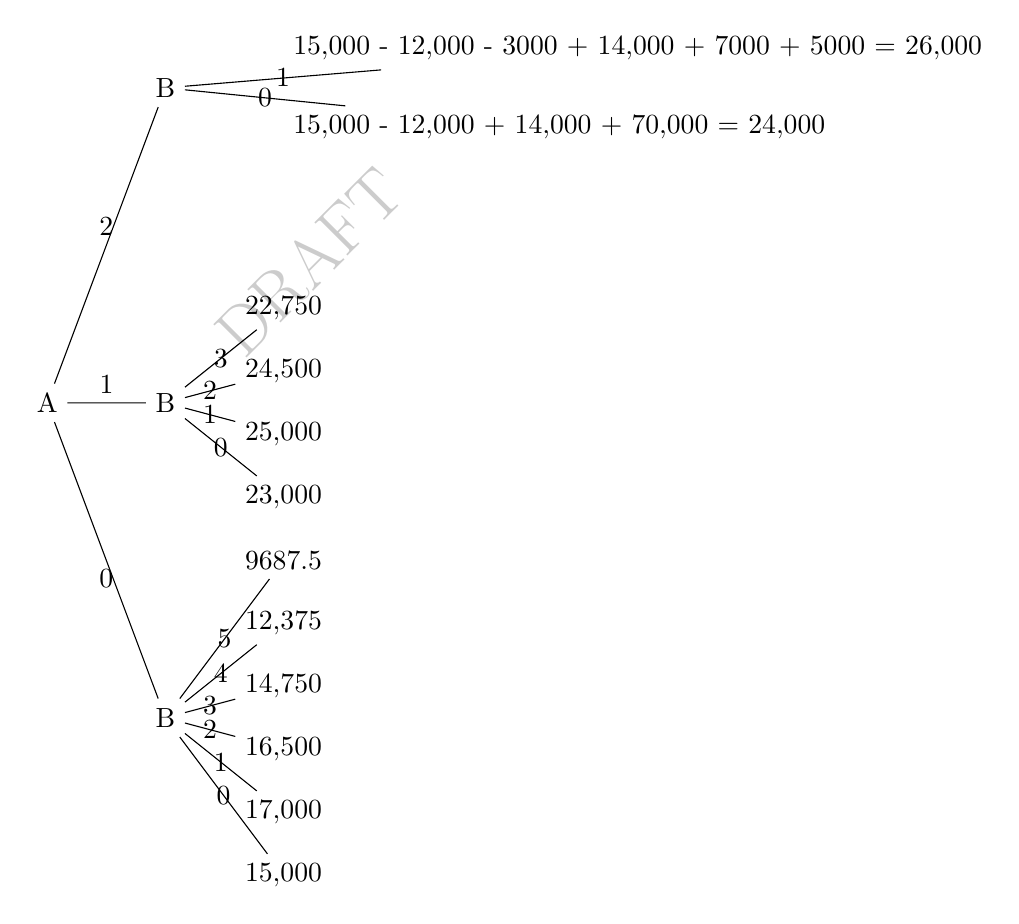
\begin{tikzpicture}
  \tikzstyle{level 1}=[sibling distance=40mm]
  \tikzstyle{level 2}=[sibling distance=8mm]
  \node {A} [grow=right]
  child{node {B} 
    child {node {\num{15000}}
    edge from parent node {0}}
    child {node {\num{17000}}
    edge from parent node {1}}
    child {node {\num{16500}}
    edge from parent node {2}}
    child {node {\num{14750}}
    edge from parent node {3}}
    child {node {\num{12375}}
    edge from parent node {4}}
    child {node {\num{9687.5}}
    edge from parent node {5}}
    edge from parent node[below] {0} }
  child {node {B}
    child {node {\num{23000}}
    edge from parent node {0}}
    child {node {\num{25000}}
    edge from parent node {1}}
    child {node {\num{24500}}
    edge from parent node {2}}
    child {node {\num{22750}}
    edge from parent node {3}}
    edge from parent node[above] {1} }
  child {node {B}
    child[sibling distance=10mm] {node[anchor=west] {\num{15000} -
    \num{12000} + \num{14000} + \num{70000} = \num{24000}}
    edge from parent node {0}}
    child[sibling distance=10mm] {node[anchor=west] {\num{15000} - 
    \num{12000} - \num{3000} + \num{14000} + \num{7000} + \num{5000} 
    = \num{26000}}
    edge from parent node {1}}
    edge from parent node[above] {2} }
  ;
\end{tikzpicture}

The company wants to make the most rational decision, so they
choose the action that maximizes the payoff. 
The company should spend the entire \$\num{15000} on robots for 
their warehouse. They should purchase two of Robot A and one of 
Robot B for a money-equivalent value of \$\num{26000}.

\end{solution}

% This exercise is OK
\item \emph{Rules for decision--making under ignorance.}
  You have the opportunity to go on a
  blind date, but you are hesitant.  You are lonely and would like to
  find the love of your life; however, you dislike awkward
  situations. Furthermore, you find it difficult to estimate the
  probability that this particular blind date will turn out to be the
  love of your life, but you know this probability is
  non-negligible. To be a little more precise, you have the following
  values: finding the love of your life is worth 1000, being in an
  awkward date situation (i.e. being on a date and knowing that you
  will not see the person again) is worth -10, and staying home
  watching Netflix is worth zero.

\begin{enumerate}
\item Formulate a decision problem for deciding whether to go on the
blind date or to stay home.
\item Use the maximin rule to solve the problem.
\item Use the minimax regret rule to solve the problem.
\end{enumerate}

\begin{solution}
\bs The decision problem can be represented with the following table.
\\[.1in]
\begin{tabular}{ccc}
 \multicolumn{3}{c}{decision matrix} \\
 & find love & lots of awkward moments \\ \cline{2-3}
go on date & 1000 & -10 \\
decline date & 0 & 0 
\end{tabular}
\\[.1in] 
The maximin rule tells you to decline the date because it has
the best of all the worst possible outcomes. To use minimax regret, we
form the regret matrix.  \\[.1in]
\begin{tabular}{ccc}
 \multicolumn{3}{c}{regret matrix} \\
 & find love & lots of awkward moments \\ \cline{2-3}
go on date & 0 & -10 \\
decline date & -1000 & 0
\end{tabular}
\\[.1in] Minimax regret tells you to go on the date because the
possibility of not finding love has the most regret.
\end{solution}


\subsubsection*{Games Against Nature}

% written by Emily
\item \emph{Gardening against nature.} A family is considering growing
  their own garden to save money on fresh vegetables. They have space
  in their yard for the garden but would need to purchase seeds and
  gardening supplies. The family is excited to grow a garden, but they
  know there are a lot of hungry rabbits in their neighborhood that
  might eat their plants before the family can harvest any vegetables
  from them. Money saved by the garden is shown in the following
  table.

\begin{tabular}{rcc}
& \multicolumn{2}{c}{State of Nature} \\
& $s_1$ & $s_2$ \\
& rabbits leave garden alone & rabbits eat garden \\ \cline{2-3}
plant garden & \$400 & -\$100\\
buy vegetables from store & 0 & 0
\end{tabular}

\begin{enumerate}
    \item If the probability that the rabbits leave the garden alone is 0.3, what decision is recommended for the family? What are the expected savings?
    
    \item The family has the option to purchase fast-growing plant seeds (the fast-growing seeds are the same price as regular seeds but they must buy the fast-growing seeds now if they want them because they are in high demand).  With these fast-growing seeds, the family can wait three more weeks to plant their garden. During that time, some scientists will finish their study on the appetites of the local rabbits, and the family will have a better idea about the probability that their garden is eaten by rabbits. They can return the seeds later for a partial refund if they do not use them.
    Let $L$ represent the event the rabbits have large appetites and let $S$ represent
    the event that rabbits have small appetites. Then
    \[
    \begin{matrix}
    P(L)=0.60, & P(s_1 \mid L)=0.15, & P(s_2 \mid L)=0.85,\\
    P(S)=0.40, & P(s_1 \mid S)=0.79, & P(s_2 \mid S)=0.21.
    \end{matrix}
    \]
    What is the optimal decision strategy if the family purchases the fast-growing seeds so they can wait and learn more about the rabbit appetites before making a decision?
    
    \item If \$40\ of the fast-growing seed purchase is non-refundable, should the family purchase the fast-growing seeds? Why or why not? What is the maximum non-refundable amount the family should pay to get the fast-growing seeds?
\end{enumerate}

\begin{solution}
\bs For part a), the expected savings when planting the garden are
\[ 400 \times 0.3  - 100 \times 0.7 = \$50. \]
The savings from not planting the garden are \$0, so based on expected value,
the best decision is to plant the garden.

For part b), if the rabbits have large appetites ($L$), then planting 
the garden would result in -\$25 of expected savings.
If the rabbits have small appetites ($S$), then planting the garden will result in \$295 
of expected savings. 

If L, \[ \$100 \times 0.15 - \$100 \times 0.85 = -\$25 \]
If S, \[ \$400 \times 0.79 - \$100 \times 0.21 = \$295 \]

Not planting will always result in \$0 of savings. 
The optimal decision strategy is to plant the garden if $S$ and buy vegetables 
from the store if $L$.

For part c), we use the optimal decision for each possible event $L$ and $S$. 
The expected savings from purchasing the fast-growing seeds
(but before actually purchasing the seeds) are
\[ \$0 \times 0.60 + \$295 \times 0.40 = \$118 \]
The maximum non-refundable amount that the family should be willing 
to pay for the fast-growing seeds is
\[ \$118 - \$50 = \$68 \]
\end{solution}

% this problem is OK
\item \emph{Using Baye's formula to update a prior belief.}
Curling is a sport in which players slide a stone over ice toward a
target. The association governing the sport has implemented drug
testing. It is believed that 15\% of all curlers use banned drugs to
enhance performance. If a player uses banned drugs, the association
may take away any prizes that the player has won; however, it
undesirable to falsely accuse someone of using banned substances.  The
utilities for each decision and state of nature are

\begin{center}
\begin{tabular}{rrrr}
& drug use & no drug use \\ \cline{2-3}
take away prizes & -100 & -1000 \\
do not & -600 & 0 
\end{tabular}
\end{center}

Notice that there is a small dis-utility for taking prizes away from a drug user
due to bad publicity for the sport. The test to detect drug use is
less than 100\% reliable. In particular, if $D$ indicates that a 
player uses banned drugs, and $+$/$-$ indicate a positive/negative
test result, then the true positive rate and the true negative rate
are
\[
P(+ \mid D) = .97 \quad \text{and} \quad P(- \mid \overline{D}) = .97,
\]
respectively, Given the utilities and the accuracy of the test, what is the best
decision if a player has a positive test result? (The association
wants to maximize expected utility.)

\begin{solution}
\bs First we update the probability of drug use via Baye's formula.
\begin{align*}
P(D \mid +) &= \frac{P(D \cap +)}{P(+)} \\
&= \frac{P(+ \mid D)P(D)}{P(+ \mid D)P(D) + P(+ \mid \overline{D})P(\overline{D})} \\
&= \frac{.97 \times .15}{.97 \times .15 + .03 \times .85} \\
&= .851
\end{align*}
and then we can compute $P(\overline{D} \mid +) = 1 - P(D \mid +) = .149$.
Using these posterior probabilities, the expected utilities are
\begin{align*}
E(\text{take away}) &= (-100)(.851) + (-1000)(.149) = -234 \\
E(\text{do not}) &= (-600)(.851) = -511
\end{align*}
The best decision is to take away prizes when a player tests positive.
\end{solution}

% Emily - expected value and sensitivity analysis
\item \emph {Decisions under risk and sensitivity analysis.}  The
  owners of a popular outdoor furniture company predict that their
  sales will double this coming year. The company is already producing
  the maximum amount of furniture possible in their current
  facility. They are considering expanding their manufacturing
  facility to accommodate the predicted increase in demand. If
  undertaken, the expansion will cost \$\num{500000}. If the demand
  doubles as predicted, revenue will increase by \$\num{800000}.  If
  the predicted increase in demand proves to be too optimistic,
  revenue will increase by only \$\num{250000}.  If the expansion is
  not undertaken, the company will lose \$\num{50000} due to
  out-of-stock orders from agitated customers.  The change in demand
  will be determined by next year's weather; more outdoor furniture is
  sold when the weather is nice.  There is a 0.55 chance of good
  weather, which will result in a doubling of demand. There is a 0.45
  chance of poor weather, which will result in only a slight increase
  in demand.

\begin{enumerate}
\item Should the manufacturing facility be expanded? The owners make
  decisions based on expected value.
\item How does the decision change with the probability of good/poor
  weather? To answer this question, you should perform a sensitivity
  analysis.
\end{enumerate}

\begin{solution}
\bs The decision table for this problem is
\begin{center}
\begin{tabular}{rrr}
      & $0.55$ & $0.45$ \\
      & good weather & poor weather \\ \hline
      expansion & \$\num{300000} & -\$\num{250000} \\
      no expansion & -\$\num{50000} & -\$\num{50000}
\end{tabular}
\end{center}

The expected payoff of each decision is
\begin{align*}
&E(\text{expansion}) = 0.55 \times \$\num{300000}
- 0.45 \times \$\num{250000} = \$\num{52500} \\
&E(\text{no expansion}) = -\$\num{50000}
\end{align*}
The company should expand the facility. As the probability of poor
weather increases, the expected value of the expansion
decreases.  Let $p$ represent the probability of poor weather.
\begin{align*}
E(\text{expansion}) &= \num{300000}(1-p) - \num{250000}p \\
&= \num{300000} - \num{550000}p
\end{align*}
The company should expand the facility as long as
\begin{align*}
E(\text{expansion}) &\geq E(\text{no expansion}) \\
\num{300000} - \num{550000}p &\geq -\num{50000} \\
-\num{5500000}p &\geq -\num{350000} \\
p &\leq \frac{7}{11} \approx .64
\end{align*}
Expanding the facility is the best decision unless the probability of
poor weather is greater than .64.
\end{solution}

\item \emph{The value of perfect information.}  You are taking a 
  date to a movie. You like horror movies but you are unsure whether
  your date likes them. You have two choices for the movie, ``The
  Burrowers'' which, despite its title, you've heard is a good movie,
  and ``A Star is Born'', which is rather safe as far as date movies
  go. Your decision problem with associated payoffs is

\begingroup
\setlength{\tabcolsep}{9pt}
\renewcommand*{\arraystretch}{2}
\begin{tabularx}{4in}{YYY}
& \multicolumn{2}{c}{Your date} \\
& likes horror movies & hates horror movies\\ \cline{2-3}
\gtcol{The Burrowers} & \gtcol{10} & \gtcol{1} \\ \cline{2-3}
\gtcol{A Star is Born} & \gtcol{4} & \gtcol{7} \\ \cline{2-3}
\end{tabularx}
\endgroup

\vspace{.2in}
\begin{enumerate}
\item Let $p$ represent the probability that your date likes horror movies. What is
  the optimal decision as a function of $p$?
\item At this point you have no information for your date's movie
  preference (even the trail of social media cannot help you) and so
  you assign $p=1/2$ as your subjective prior probability. Suppose
  that the date's best friend will tell you for sure whether your date
  likes horror movies, but this person is not so nice and wants to be
  paid. If the payoffs represent dollar amounts then how much are you
  willing to pay this person for perfect information? \label{ex:pi}
\end{enumerate}

\begin{solution}
  \bs Choose ``The Burrowers'' if
  \begin{align*}
    10p + (1-p) &> 4p + 7(1-p)\\
    9p + 1 &> -3p + 7\\
    12p &> 6\\
    p &> 1/2
  \end{align*}

  Regarding part \ref{ex:pi}, if you knew that your date liked horror
  movies you would choose ``The Burrowers'' for a pyoff of \$10 and if
  you knew the opposite then you would choose ``A Star is Born'' for a
  payoff of \$7. The expected payoff with perfect information, that
  is, before you actually receive the information, is
  \[ \frac{1}{2}(10) + \frac{1}{2}(7) = 8\frac{1}{2} \]
  Without the information your expected payoff is $\$5 \frac{1}{2}$ (for either
  choice). You would be willing to pay at most
  \[ \$8.50 - \$5.50 = \$3 \]
  for the perfect information.

\end{solution}

% written by Emily
\item \emph{Quality control and the value of perfect information.} 
  A worker in a factory producing potato chips notices that a small 
  bolt is missing off of a piece of equipment in the packaging 
  area and determines that it fell into a bag before it was
  sealed. Two pallets worth of chips have been produced since 
  the last routine check was performed determining that the 
  bolt was in place. The worker does not want to throw away all
  bags of chips that the bolt could possibly be in, so he decides
  to search for the bolt. He has to decide if he should start 
  searching bags on pallet one or pallet two. If the bolt fell into
  a bag on pallet one and he searches bags on pallet one, there is a 0.5 
  chance of finding it by the end of the day. If the bolt fell into 
  a bag on pallet two and he searches pallet two, there is a 0.8 chance
  that he finds the bolt. The worker's prior probability that the bolt
  is in a bag on pallet one is 0.7 (he thinks it was loose from some work done earlier in the day and fell off right away).

\begin{enumerate}
\item The worker only has time to search one pallet per day. 
  In which pallet, one or two, should he look for the bolt?  
  The worker wants to maximize his
  probability of finding the bolt. 
\item Suppose that at the end of the day when the worker goes home,
  he has not found the bolt yet. Which pallet should he 
  search on day 2?
  \emph{Hint}: First update the prior probabilities that the bolt is
  in pallet one/two.
\item Suppose that on the second day, just before the worker begins
  to
  search for the bolt, a security guard approaches and tells him
  that he has access to security camera footage that would reveal when 
  the bolt fell into a bag (revealing which pallet the bolt is in).
  How much should the worker be willing to pay for this perfect 
  information?  Note that the ``units'' for the payment are in 
  terms of probabilities.
\end{enumerate}

\begin{solution}
\bs
Let $A$ be the event that the bolt is in pallet one and let $B$ be the event
that the bolt is in pallet two. Also, let $F_A$ represent the event that the worker
finds the bolt in pallet one (and similarly define $F_B$). We are given the
following.
\begin{align*}
  P(F_A \mid A) = 0.5 &\qquad P(\overline{F}_A \mid A) = 0.5 \\
  P(F_B \mid B) = 0.8 &\qquad P(\overline{F}_B \mid B) = 0.2 \\
\end{align*}

The worker's decision problem is

\begingroup
\setlength{\tabcolsep}{9pt}
\renewcommand*{\arraystretch}{2}
\begin{tabularx}{3.25in}{YYYY}
& & \multicolumn{2}{c}{Nature} \\
& & $0.7$ & $0.3$ \\
& & $A$ & $B$  \\ \cline{3-4}
\multirow{2}{.9in}{Worker} & \gtcol{Look in A} & \gtcol{.5} & \gtcol{0} \\ \cline{3-4}
& \gtcol{Look in B} & \gtcol{0} & \gtcol{.8} \\ \cline{3-4}
\end{tabularx}
\endgroup
\vspace{.2in}

The best option is to look in pallet one. He will find the bolt on the first
day with probability $0.7 \times 0.5 = 0.35$.

On the second day, the worker's belief that the bolt is in pallet one is updated to
\begin{align*}
  P(A \mid \overline{F}_A) &= \frac{P(\overline{F}_A \mid A)P(A)}{P(\overline{F}_A \mid A)P(A) + P(\overline{F}_A \mid B)P(B)}\\
                           &= \frac{0.5 \times 0.7}{0.5 \times 0.7 + 1 \times 0.3} \\
                           &= 0.538
\end{align*}
which implies that $P(B \mid \overline{F}_A) = 1 - 0.538 = 0.462$. On day two,
the worker's decision problem is

\begingroup
\setlength{\tabcolsep}{9pt}
\renewcommand*{\arraystretch}{2}
\begin{tabularx}{3.25in}{YYYY}
& & \multicolumn{2}{c}{Nature} \\
& & $0.538$ & $0.462$ \\
& & $A$ & $B$  \\ \cline{3-4}
\multirow{2}{.9in}{Worker} & \gtcol{Look in A} & \gtcol{.5} & \gtcol{0} \\ \cline{3-4}
& \gtcol{Look in B} & \gtcol{0} & \gtcol{.8} \\ \cline{3-4}
\end{tabularx}
\endgroup
\vspace{.2in}

and his best option is to look in pallet two. The worker will find the bolt with probability
\[ 0.462 \times 0.8 = 0.37\]

With perfect information, but \emph{before} receiving the information, the worker's
expected value for the probability of finding the bolt is
\[ 0.5 \times 0.538 + 0.8 \times 0.462 = 0.639 \]
and in terms of probability ``units'', he should be willing to pay
\[ 0.639 - 0.37 = 0.269 \]
for the information.

\end{solution}


% this problem is OK.
\item \emph{Planting crops and the value of imperfect information.} A
  farmer can plant one of four crops. The yield in bushels per acre
  depends on the particular crop planted and the weather during the
  growing season. Regarding crop yields, the weather can be
  categorized as dry, moderate, or wet. The estimated crop yields,
  commodity prices, and weather forecast are provided in the table
  below.

\begin{center}
\begin{tabular}{lcccc}
& dry & moderate & wet & \$/bushel \\ \hline
crop 1 & 30 & 50 & 60 & \$3.00 \\
crop 2 & 25 & 30 & 40 & \$4.50 \\
crop 3 & 40 & 35 & 35 & \$3.00 \\
crop 4 & 60 & 60 & 60 & \$1.50 \\ \hline
forecast & .2 & .5 & .3 & 
\end{tabular}
\end{center}

\begin{enumerate}
\item If the farmer maximizes expected monetary value, which crop
should she plant and what is her expected revenue per acre?

\item Suppose that the farmer could pay an oracle to tell her
with certainty which category of weather would occur during
the growing season. How much should the farmer be willing to 
pay for this perfect information? Your answer should be in terms
of \$/acre. \label{b}

\item Now suppose a start-up company that specializes in predictive
  modeling announces a new machine learning algorithm for weather
  forecasting. The predictions from the model are good, but not
  perfect.  In particular, the company advertises the following
  accuracy for the weather forecasting model. \label{c}

\begin{center}
\begin{tabular}{clccc}
& & \multicolumn{3}{c}{actual} \\
& & dry & moderate & wet \\ \cline{2-5}
\parbox[t]{2mm}{\multirow{3}{*}{\rotatebox[origin=c]{90}{model}}} & dry & .9 & .1 & .05 \\
& moderate & .05 & .8 & .05 \\
& wet & .05 & .1 & .9 
\end{tabular}
\end{center}

For example, if the weather actually turns out to be dry, the model
would have predicted dry weather with probability .9, moderate weather
with probability .05, and wet weather with probability .05. How much
should the farmer be willing to pay (again in \$/acre) for this
less-than-perfect prediction of the weather? Settle in with a cup of
coffee: this part requires some work. Here is a strategy.
\begin{enumerate}[i)]
\item Develop a notation, e.g., $x$ indicates the weather during the growing season,
and $x'$ indicates the prediction, where $x$ is dry, moderate, or wet.

\item Use Baye's formula to compute the posterior probabilities for
  each weather category given the predictions, e.g. you want to know
  $P(d \mid d')$, $P(m \mid d')$, etc.

\item Determine the expected payoff for each case that the prediction is
dry, moderate, and wet.

\item The expected value of the prediction (i.e. the expected value of the
less-than-perfect information) is the difference between the expected payoff
with the information and without it.
\end{enumerate}

\end{enumerate}

\begin{solution}
\bs Considering the estimated commodity prices, the payoff table and expected
values in \$/acre for each crop are

\begin{center}
\begin{tabular}{lrrrr}
& dry & moderate & wet & $E(\text{payoff})$ \\ \hline
crop 1 & 90 & 150 & 180 & \$147 \\
crop 2 & 112.5 & 135 & 180 & \$144 \\
crop 3 & 120 & 105 & 105 & \$108 \\
crop 4 & 90 & 90 & 90 & \$90 
\end{tabular}
\end{center}

To maximize expected monetary value the farmer should plant crop 1 and
expect \$147/acre of revenue. For part~\ref{b}, if she knew for
certain that the weather would be dry, moderate, or wet, then she
would plant crop 3 with revenue \$120 per acre, crop 1 with revenue
\$150 per acre, and crop 1 (or 2) with revenue \$180 per acre,
respectively. Prior to learning the perfect information, the farmer's
expected payoff with the new information is
\[
.2 \times \$120 + .5 \times \$150 + .3 \times \$180 = \$153
\]
and so the value of the perfect information is worth no more than
\[
\$153 - \$147 = \$6~\text{per acre}
\]

Now for part~\ref{c}, the likelihoods are provided as follows
(using the notation given in the problem description).
\[
\begin{matrix}
P(d' \mid d)=.9 & P(m' \mid d)=.05 & P(w' \mid d)=.05 \\
P(d' \mid m)=.1 & P(m' \mid m)=.8 & P(w' \mid m)=.1 \\
P(d' \mid w)=.05 & P(m' \mid w)=.05 & P(w' \mid w)=.9 \\
\end{matrix}
\]

Using Baye's formula to compute the posterior probabilities, we get
\begin{align*}
P(d \mid d') &= \frac{P(d \cap d')}{P(d')} \\
&= \frac{P(d' \mid d)P(d)}{P(d' \mid d)P(d) + P(d' \mid m)P(m) + P(d' \mid w)P(w)} \\
&= \frac{(.9)(.2)}{(.9)(.2) + (.1)(.5) + (.05)(.3)} \\
&= .735
\end{align*}
and in a similar manner 
\[
\begin{matrix}
& P(m \mid d')=.204 & P(w \mid d')=.061 \\
P(d \mid m')=.024 & P(m \mid m')=.941 & P(w \mid m')=.035 \\
P(d \mid w')=.03 & P(m \mid w')=.152 & P(w \mid w')=.818 \\
\end{matrix}
\]
The expected monetary values given the predictions are

\begin{center}
\begin{tabular}{lrrr}
& $E(\text{dry})$ & $E(\text{moderate})$ & $E(\text{wet})$ \\ \hline
crop 1 & \$108 & 150 & 173 \\
crop 2 & 121 & 136 & 171 \\
crop 3 & 116 & 105 & 105 \\
crop 4 & 90 & 90 & 90
\end{tabular}
\end{center}

If the prediction is dry, the farmer would plant crop 2 for an
expected revenue of \$121 per acre. Similarly for predictions
of moderate and wet, she would plant crop 1 with expected revenue
\$150 per acre and crop 1 with expected revenue \$173 per acre,
respectively. Prior to obtaining the weather prediction,
the expected value of having the prediction is 
\begin{align*}
E(\text{payoff}) &= \$121 \times P(d') + \$150 \times P(m') + \$173 \times P(w') \\
&= \$121 \times .245 + \$150 \times .425 + \$173 \times .33 \\
&= \$150.50
\end{align*}
Note that the unconditional probabilities of the predictions are obtained
using the formula for total probability and they were computed during the
application of Baye's formula. The value of the less-than-perfect
informtaion is 
\[
\$150.50 - \$147 = \$3.50~\text{per acre}
\]
\end{solution}

% decisions over time
% this problem is OK.
\item \emph{The break-up.} You are considering
  breaking up with your boy(girl)friend; however, you know that
  he(she) may break up with you. Your utility is higher if you end
  the realtionship, but it's Friday and you have joint plans for the
  weekend. Here is the situation: on Friday (and possibly Saturday)
  you need to decide to either stay in the relationship, or end it.
  \begin{compactitem}[i)]
    \item \emph{On Friday:}
  If you decide to end the relationship your payoff is one
  (and your done.) If you stay in the relationship then a random
  chance event happens where your boy(girl)friend ends the relationship
  with probability 0.25 and stays with probability 0.75.
\item \emph{On Saturday:} If you end the relationship your
  payoff is 3 (and your done.) If you stay then a chance event happens
  where your boy(girl)friend ends the relationship with probability
  0.5 and stays with probability 0.5.
\end{compactitem}
If you stay in the relationship until Sunday, then you will definitely
end it and your payoff is 4. If, on Friday or Saturday, your boy(girl)friend
ends the relationship then your payoff is one.

Use backward induction to determine a policy for ending/staying that
will maximize your expected payoff.

\begin{solution}
  \bs The decision tree is shown below. Working backwards, the expected
  value of ``stay'' on Saturday is 2.5, so the best decision is ``exit'',
  for a payoff of 3. On Friday, the expected value of ``stay'' is 2.5,
  which is better than ``exit'' with a payoff of 1. So, the policy that
  maximizes expected payoff is to stay in the relationship on Friday and
  exit the relationship on Saturday.

\vspace{.2in}
\begin{center}
%\resizebox{.5\textwidth}{!}{%
  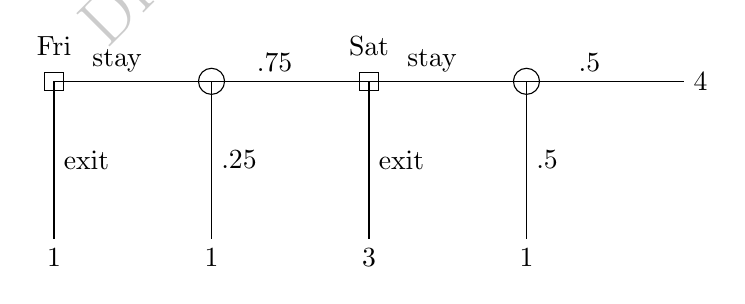
\begin{tikzpicture}
    \draw (0,0) -- (8,0)
    node[pos=.1,anchor=south] {stay}
    node[pos=.35,anchor=south] {.75}
    node[pos=0.6,anchor=south] {stay}
    node[pos=.85,anchor=south] {.5}
    node[right] {4};
    \draw (0,0) -- (0,-2) node[pos=0.5,anchor=west] {exit} node[below] {1};
    \draw (2,0) -- (2,-2) node[pos=.5,anchor=west] {.25} node[below] {1};
    \draw (4,0) -- (4,-2) node[pos=0.5,anchor=west] {exit} node[below] {3};
    \draw (6,0) -- (6,-2) node[pos=0.5,anchor=west] {.5} node[below] {1};
    \node[draw] at (0,0) {};
    \node[circle,draw] at (2,0) {};
    \node[draw] at (4,0) {};
    \node[circle,draw] at (6,0) {};
    \node[anchor=south] at (0,0.2) {Fri};
    \node[anchor=south] at (4,0.2) {Sat};
\end{tikzpicture}%}
\end{center}
\end{solution}

% written by Emily
\item \emph{An optimal strategy for a family visit.}  
Parker's family is 
coming to visit him for two days. He is going to plan an activity 
for each day, and he must decide if it will be an indoor
or outdoor activity. What he chooses the first day (indoor or
outdoor) can differ from what he chooses the second day. He wants
his family to enjoy whatever he chooses. There are many factors
that determine if Parker's family enjoys an activity such as
weather, how they are feeling, and their interest level.
If Parker picks an outdoor activity, the probability that
his family will enjoy the activity is $p_e$ and the probability
that they do not enjoy the activity is $1-p_e$.
If Parker picks an indoor activity, the probability that his family will 
enjoy the activity is $p_h$ and the probability that they will not 
is $1-p_h$. 
To measure the success of the visit, Parker has come up with the 
following scoring system: an outdoor activity that his family enjoys 
is worth 2 points, an indoor activity that his family enjoys is worth 
1 point, and any activity that his family does not enjoy is worth 
zero points.
Let $p_e=0.4$ and let $p_h=0.75$. 
Which type of activity should Parker select for the first day
of the visit, indoor or outdoor? What about the second day? 
In other words, what is the
plan that will maximize Parker's expected 
payoff for the 2-day visit?

\begin{solution}
  \bs The optimal strategy for Parker is to plan an outdoor
  activity for both days.
  Please see the attached decision tree. 
\end{solution}

\subsubsection*{Games Against an Opponent}

% written by Emily
\item \emph{Elimination of dominated strategies.}
Two street vendors, A and B, are located near a major tourist attraction. 
The proportion of customers
captured by each vendor depends on the merchandise sold by that vendor and by
her competitor. A customer gained by one is lost to the other. Each vendor
can stock one of the following: clothing, ice cream, or souvenirs.
The possible strategies and proportion of customers captured are as follows.

\begin{tabular}{l}
If both shops sell souvenirs, A captures 75\% of the customers.\\
If both shops sell clothing, A and B split the customers evenly.\\
If both shops sell ice cream, A and B split the customers evenly.\\
If B sells ice cream and A sells souvenirs, A captures 10\%.\\
If B sells clothing and A sells ice cream, A captures 90\%.\\
If B sells souvenirs and A sells clothing, A captures 10\%.\\
If A sells clothing and B sells ice cream, A captures 100\%.\\
If A sells souvenirs and B sells clothing, A captures 75\%.\\
If A sells ice cream and B sells souvenirs, A captures 40\%.
\end{tabular}

\setlength{\parindent}{0cm}
Model the decision of each vendor as two-person zero-sum game
and find a solution by elimination of dominated strategies.

\begin{solution}
\bs The game is

\begingroup
\setlength{\tabcolsep}{9pt}
\renewcommand*{\arraystretch}{2}
\begin{tabularx}{4.5in}{YYYYY}
& & \multicolumn{3}{c}{B} \\
& & clothing & ice cream & souvenirs \\ \cline{3-5}
\multirow{3}{.25in}{A} & \gtcol{clothing} & \gtcol{.50} & \gtcol{1} & \gtcol{.10} \\ \cline{3-5}
& \gtcol{ice cream} & \gtcol{.90} & \gtcol{.50} & \gtcol{.40} \\ \cline{3-5}
& \gtcol{souvenirs} & \gtcol{.75} & \gtcol{.10} & \gtcol{.25} \\ \cline{3-5}
\end{tabularx}
\endgroup
\vspace{.1in}

For A, ice cream strictly dominates souvenirs and for B, souvenirs
strictly dominates clothing, leaving a $2 \times 2$ game.

\begingroup
\setlength{\tabcolsep}{9pt}
\renewcommand*{\arraystretch}{2}
\begin{tabularx}{4in}{YYYY}
& & \multicolumn{2}{c}{B} \\
& & ice cream & souvenirs \\ \cline{3-4}
\multirow{2}{.25in}{A} & \gtcol{clothing} & \gtcol{1} & \gtcol{.10} \\ \cline{3-4}
& \gtcol{ice cream} & \gtcol{.50} & \gtcol{.40} \\ \cline{3-4}
\end{tabularx}
\endgroup
\vspace{.1in}

Now for B, souvenirs dominates ice cream. Then, A will choose to sell
ice cream over clothing. So, the best strategies for A and B are to
sell ice cream and souvenirs, respectively.  Using this pair of
strategies, A will capture 40\% of the customers.
\end{solution}

% written by Emily to replace Goldsen and Kershaw battle of words
\item \emph{A two-person zero-sum game.}  A professional football
  player believes that the team he plays for should be allocating more
  money to the salaries of the players, so he wants his contract to be
  changed to pay him more. His two options are to play in the upcoming
  season or not play in the upcoming season and hope the team will
  negotiate with him. The team knows that he is a valuable player but
  does not want to pay him more or go through the process of
  negotiations. The team has come up with three options to deal with
  the situation: negotiate, refuse to negotiate and play the season
  without him, or increase the player's salary by a set amount with no
  other negotiations. Keep in mind that the player wants to maximize
  his salary, and the team wants to minimize their costs, which means
  keep salaries as low as possible. The utilities/payoffs to
  the player and to the team are described next.

  If the player plays and the team does not negotiate, the player's
  salary will not change.  If the player does not play and the team
  does not negotiate, the player will find a different job as a
  broadcaster for a payoff of 1 because he is such a well-known
  person. This is bad publicity for the team and hurts their jersey
  sales.  If the player plays but the team still negotiates, the
  player will end up with a payoff of 3.  If the player had
  chosen to not play and the team negotiates, the negotiations will go
  poorly and the player will end up with a payoff of -2 for having to
  deal with costs related to poor publicity.  If the team decides
  increase the player's salary with no negotiations, the player will
  end up with a payoff of 2 no matter what he chooses to do.


  Formulate the 2-by-3 game and determine the best strategy for the
  player and for the team.  Who is most likely to come out ahead in
  this situation?
  
\begin{solution}
\bs The game is

\begingroup
\setlength{\tabcolsep}{9pt}
\renewcommand*{\arraystretch}{2}
\begin{tabularx}{4.5in}{YYYYY}
& & \multicolumn{3}{c}{Team} \\
& & negotiate & don't negotiate & increase salary \\ \cline{3-5}
\multirow{2}{.5in}{Player} & \gtcol{play} & \gtcol{3} & \gtcol{0} & \gtcol{2} \\ \cline{3-5}
& \gtcol{don't play} & \gtcol{-2} & \gtcol{1} & \gtcol{2} \\ \cline{3-5}
\end{tabularx}
\endgroup
\vspace{.1in}

The team's strategy of a set
increase is dominated by the strategy to not negotiate, so there is no
reason that they would chose to offer a pre-determined
increase without negotiations. The reduced game is

\begingroup
\setlength{\tabcolsep}{9pt}
\renewcommand*{\arraystretch}{2}
\begin{tabularx}{4in}{YYYY}
      & & \multicolumn{2}{c}{Team} \\
      & & {negotiate} & {don't negotiate} \\ \cline{3-4}
      \multirow{2}{.5in}{Player} & \gtcol{play} & \gtcol{3} & \gtcol{0} \\ \cline{3-4}
      & \gtcol{don't play} & \gtcol{-2} & \gtcol{1} \\ \cline{3-4}
\end{tabularx}
\vspace{.1in}
\endgroup

Since there is no saddle point, the best strategies for the player and
for team are mixed. The player should mix the strategies ``play'' and
``don't play'' in the ratio 1:1. The team should mix the strategies
``negotiate'' and ``don't negotiate'' in the ratio 1:5.  Using the
player's mixing ratios against the team's strategy of ``negotiate''
the value of the game is computed as
\[
\frac{1 \times (3) + 1 \times (-2)}{2} = 1/2.
\]
The player is more likely to come out ahead. 
\end{solution}
  
% written by Emily to replace cops and robbers
\item \emph{Marketing strategies.} Two peanut butter companies,
  Doodle's and Lola's, are deciding on their marketing strategy for
  the upcoming year. They know that they are each other's main
  competitor and that the demand for peanut butter is relatively
  constant, so a gain in sales for Doodle's is a loss of sales for
  Lola's. Each company has their standard packaging for peanut butter
  and a new innovative packaging for peanut butter. Both companies
  may produce and sell both types of packaging.  If both
  companies choose to market only their innovative packaging, Doodle's
  will gain an extra 2\%\ of the market's sales.  If both companies
  choose to market their standard packaging, Doodle's will loose 2\%\
  of the market.  If Doodle's markets their innovative product and
  Lola's markets their standard product, Doodle's will gain 10\%\
  of the market.  If Lola's markets their innovative product and
  Doodle's markets their standard product, Doodle's will gain 8\%\
  of the market.
 
\begin{enumerate}
\item Formulate this decision problem as a two-person zero-sum game
  and determine the optimal marketing strategy for each company. Note
  that they are able to change their advertising throughout the year,
  so a mixed strategy is possible.
\item Compute the value of the game. \label{val}
\item Suppose that a member of Doodle's marketing team quits her
  job and goes to work for Lola's. She tells her new co-workers
  about the strategy that Doodle's is planning to use. She is even able to
  tell them the probabiliites with which Doodle's will market their
  standard product and their innovative product. Lola's marketing
  team now knows that Doodles is more likely to market the innovative
  product than the standard product. Armed with this knowledge, they
  choose to only market their standard product, thinking that this
will improve their payoff. Is Lola's argument
  valid? In other words, does the value of the game change if
  Lola's knows Doodle's optimal strategy?
\label{knowledge}
\end{enumerate}

\begin{solution}
\bs The game is

\begingroup
\setlength{\tabcolsep}{9pt}
\renewcommand*{\arraystretch}{2}
\begin{tabularx}{3.25in}{YYYY}
& & \multicolumn{2}{c}{Lola's} \\
& & standard & innovative \\ \cline{3-4}
\multirow{2}{.5in}{Doodle's} & \gtcol{standard} & \gtcol{-2} & \gtcol{8} \\ \cline{3-4}
& \gtcol{innovative} & \gtcol{10} & \gtcol{2} \\ \cline{3-4}
\end{tabularx}
\endgroup
\vspace{.1in}

Note that there is no saddle point, and so the best strategy is mixed.
Doodle's should mix the strategies standard and innovative
in the ratio 4 to 5, while Lola's should mix their strategies of
standard to innovative in the ratio 1 to 2.  The corresponding
probabilities are $(4/9,\,5/9)$ for Doodle's and $(1/3,\,2/3)$ for
Lola's.

To compute the value of the game, note that when
Doodle's markets the standard product, they receive a payoff of -2
with probability 1/3 and payoff of 8 with probability 2/3.  The value
of the game is
\[ \frac{1 \times -2 + 2 \times 8}{3} = \frac{14}{3} = 4.67 \]
On average Doodle's comes out ahead.

Regarding part \ref{knowledge}), the team's thought process is not
valid.  As long as one player sticks to the optimal mixed strategy,
the value of the game does not change.
\end{solution}

% written by Emily to replace the silver dollar
\item \emph{The birthday gift.} Liam's birthday is coming up and he
  can't wait to see what he will get as a gift. Liam's parents want
  the gift to be a surprise, but they always hide gifts in either the
  kitchen or the basement. Liam plans to search for the gift when his
  parents are busy, but he knows that even if he searches the room
  that contains the gift, he may not find it. If the gift is hidden in
  the kitchen and Liam searches the kitchen, he will find the gift
  with probability 0.75.  If the gift in hidden in the basement and he
  searches the basement, then he will find it with probability 0.5.
  If he searches the wrong room, there is no way he will find the
  gift. Assume that the payoff to Liam for finding the gift early is
  the same as the payoff to the parents of keeping the gift a
  surprise.  Formulate this game as a two-person, zero-sum game. Liam
  is the row player and his parents are the column player. Find the
  optimal strategies for both players. \label{sda}

\begin{solution}
  \bs Liam has two possible actions for this game: search the kitchen
  or search the basement. His parents also have two options: hide the
  gift in the kitchen or hide the gift in the basement.  The game is

\begingroup
\setlength{\tabcolsep}{9pt}
\renewcommand*{\arraystretch}{2}
\begin{tabularx}{4in}{YYYY}
& & \multicolumn{2}{c}{Parents} \\
& & hide in kitchen & hide in basement \\ \cline{3-4}
\multirow{2}{.5in}{Liam} & \gtcol{search kitchen} & \gtcol{3/4} & \gtcol{0} \\ \cline{3-4}
& \gtcol{search basement} & \gtcol{0} & \gtcol{1/2} \\ \cline{3-4}
\end{tabularx}
\endgroup
\vspace{.1in}

and the optimal strategy is the same for both players. Each
should play a mixture of $(2/5,~3/5)$.
\end{solution}

% written by Emily
\item \emph{Workforce staffing.}  A salon is trying to decide how many
  stylists they should have available for walk-in customers. The
  hourly walk-in demand is specified by the following probability
  distribution, where $p_n$ is the probability of having $n$ customers
  in one hour.

\vspace{.2in}
\begin{tabular}{r|rrrrr}
$n$ & 1 & 2 & 3 & 4 & 5 \\ \hline
$p_n$ & .10 & .20 & .35 & .25 & .10 \\
\end{tabular}

\vspace{.2in} Each stylist costs the salon \$20\ per hour.  If a
stylist has a customer that hour, the salon will charge the customer
\$45\ for service.  Each customer requires about an hour of time from
a stylist.  If a stylist does not have a customer that hour, he/she
will complete a different task in the salon which adds \$9\ of
value. If all stylists are busy with a customer and an additional
customer arrives, that customer will be turned away and will go to a
different salon. How many stylists should be available each hour in
order to maximize profit for the salon?

\begin{solution}
  \bs Let $Q$ represent the available number of stylists (quantity)
  and let $z$ represent the demand. There are two situations.  First,
  if $Q \geq z$
\begin{align*}
E(\text{profit}) &= 45z - 20Q + 9(Q-z) \\
&= 36z - 11Q
\end{align*}
Otherwise if $Q < z$, then
\begin{align*}
E(\text{profit}) &= 45Q - 20Q\\
&= 25Q
\end{align*}

We use the distribution of demand to compute the expected profit
for each possible level of staffing.
\begin{center}
\begin{tabular}{rr|rrrrrr}
& & \multicolumn{5}{c}{$z$} & \\
& & .1 & .2 & .35 & .25 & .1 & \\
& & 1 & 2 & 3 & 4 & 5 &  $E(\text{payoff})$ \\ \hline
\multirow{5}{*}{$Q$} & 1 & 25 & 25 & 25 & 25 & 25 & 25 \\
& 2 & 14 & 50 & 50 & 50 & 50 & 46.4 \\
& 3 & 3 & 39 & 75 & 75 & 75 & 60.6 \\
& 4 & -8 & 28 & 64 & 100 & 100 & 62.2 \\
& 5 & -19 & 17 & 53 & 89 & 125 & 54.8
\end{tabular}
\end{center}

The best decision is to have 4 stylists available.
\end{solution}

\subsubsection*{Utility Theory}

% Written by Emily
% Expected Utility Theorem
\item \emph{Expected utility of a day off.}  Utilities are the basis
  for making rational decisions.  Sydney has the day off from work and
  she is trying to decide what to do. Her top three options and their
  utilities are:

\begin{tabular}{lr}
  option & utility \\ \hline
  go to the beach & 100\\
  go hiking & 75\\
  stay home and watch movies & 50
\end{tabular}

With only this information, Sydney would choose to go to the beach for
the day. However, there is some uncertainty (or risk) in Sydney's
decision. The weather and the people she runs into at the beach or
while hiking impact her utility.  Sydney does not enjoy being outside
when it is raining.  If it rains while she is at the beach, her
utility is decreased by 80.  If it rains while she is hiking, her
utility is decreased by 30.  On the other hand, Sydney enjoys running
into friends. If she runs into a friend at either the beach or on the
hiking trail, it will increase Sydney's utility by a factor of 1.5
(after any disutility has been appplied).

At the beach, it is rainy 40\% of the time and Sydney has a 30\%
chance of running into a friend.  On the hiking trail, it is rainy
20\% of the time and she has a 50\% chance of running into a friend.
Compute Sydney's expected utilities for each option. What is the
``rational'' decision for Sydney?

With this exercise, there are three points to be made:
\begin{enumerate}
\item Rational choice means that agents (like Sydney) make decisions 
    that maximize their utility (or payoff, or happiness). It doesn't 
    mean that agents only care about themselves. Agents have 
    preferences over states of the world. An agent might have a preference 
    for making another agent happy, and that would be reflected in her 
    utility for that state of the world.
\item Each agent has a utility function that maps states of the world
    to real numbers that represent the agent's level of happiness.
\item When there is uncertainty over which state will occur, then
    an agent's utility is her expected utility.
\end{enumerate}

\begin{solution}
\bs We must calculate the expected utility for each possible decision.
The expected utility of going to the beach is:
\begin{align*}
E(\text{utility}) &= 100 - 80 \times 0.40 + 
(100 - 80 \times 0.40) \times 0.50 \times 0.30 \\
&= 78.20
\end{align*}
The expected utility of going hiking is:
\begin{align*}
E(\text{utility}) &= 75 - 30 \times 0.20 + (75 - 30 \times 0.20) \times 0.50 \times 0.50 \\
&= 86.25
\end{align*}
The expected utility of staying home watching movies is 50 because it
is influenced by neither the weather nor running into friends. The
``rational'' decision for Sydney is to go hiking.
\end{solution}

\item \emph{Attitudes toward risk.}  Consider the following scenarios
  for Alice and Bob. Then, draw reasonable utility functions for each
  person. Alice's utility function should be in the range zero to
  \$100K.  Bob's should be from zero to \$40.

  Alice has worked hard to save \$25K for a down payment on a
  house. She is ready to buy the house, but just before closing, she
  is offered the following hot tip. If she invest invests \$25K in a
  cryptocurrency, there is an 80\% chance that she will make \$50K
  within one month, but a 20\% chance that she will lose everything.
  The expected monetary value of the opportunity is
  \[
  0.8 \times \$75\text{K} - 0.2 \times \$25\text{K} = \$55\text{K},
  \]
  but Alice makes the \$25K down payment even though the EMV of the
  investment is higher. The certainty of getting the house is worth
  more to her than the uncertain gain from the investment.

  Bob has \$20 in his possession. He \emph{really} wants to see the
  show at First Avenue, but tickets cost \$40. Over on 7th Street,
  someone comes along and offers Bob the following gamble.
\begin{quote}
  Put in \$20. Roll a die. If the die comes up ``6'', then the player
  wins \$20. If the die comes up any other number the player loses the
  \$20.
\end{quote}
If Bob is lucky enough to win the gamble, he would have \$40 for the
ticket. The expected monetary value of the gamble is
  \[
  \frac{1}{6} \times \$40 - \frac{5}{6} \times \$20 = -\$10,
  \]
  but Bob takes the bet because the chance to see the show is worth
  more to him than having \$20 and \emph{not} seeing the show.

\begin{solution}
  \bs The important point is the general shape of the utility
  functions, not the magnitudes of the utilities. Alice is risk-averse
  and Bob is risk-seeking.

\begin{minipage}{.49\textwidth}
\resizebox{\textwidth}{!}{%
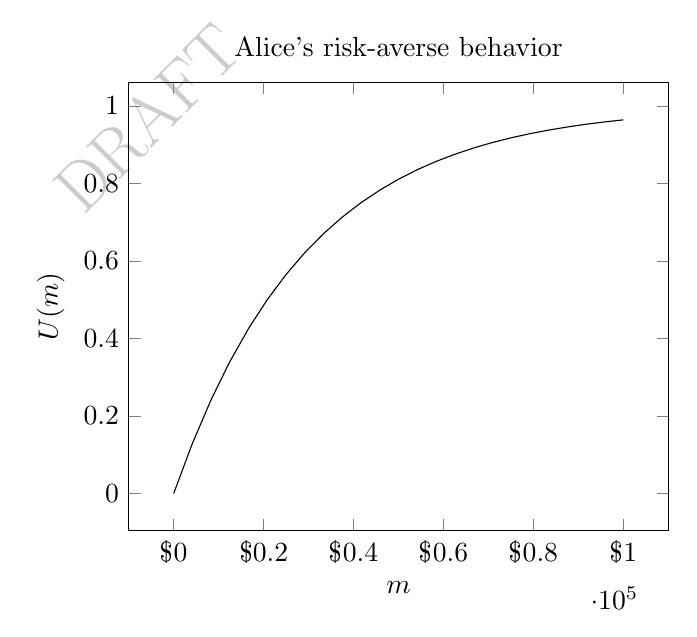
\begin{tikzpicture}
\begin{axis}[
xlabel={$m$},
ylabel={$U(m)$},
xticklabel={\$$\pgfmathprintnumber{\tick}$},
title=Alice's risk-averse behavior,
]
\addplot[domain=0:100000] {1 - exp(-x/30000)};
\end{axis}
\end{tikzpicture}}
\end{minipage}
\hfill
\begin{minipage}{.49\textwidth}
\resizebox{\textwidth}{!}{%
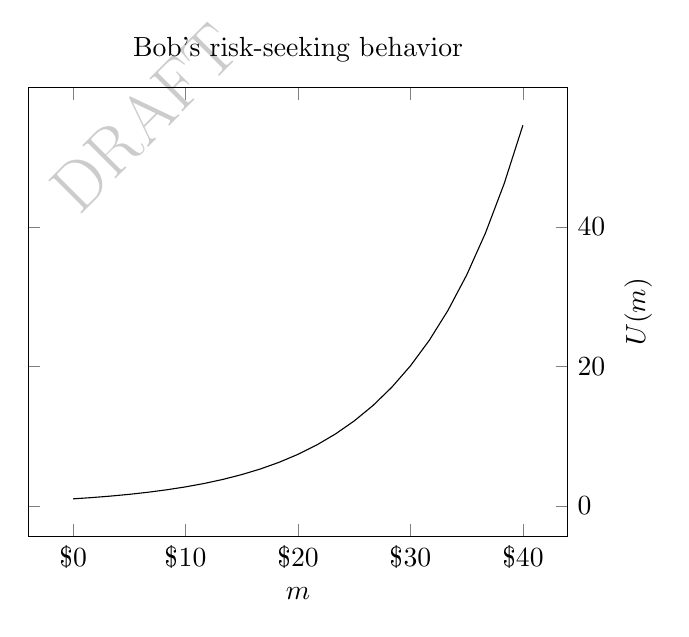
\begin{tikzpicture}
\begin{axis}[
xlabel={$m$},
ylabel={$U(m)$},
xticklabel={\$$\pgfmathprintnumber{\tick}$},
title=Bob's risk-seeking behavior,
yticklabel pos=right,
]
\addplot[domain=0:40] {exp(x/10)};
\end{axis}
\end{tikzpicture}}
\end{minipage}

\end{solution}

\item \emph{Registering for classes.} You are deciding to register for
  one of two classes, IE 5571 or IE 5591. If you register for IE 5571
  you know that you will get a B for sure, but IE 5591 is a lottery
  because the department has not yet decided who will teach the
  class. If Professor England teaches the class then you will get an
  A, but if Professor Doroudi teaches the class then you will get a
  C. You will not know the identity of the instructor until class
  begins and you cannot withdraw from the course once registered. The
  points associated with the letter grades are

\begingroup
\renewcommand{\arraystretch}{1}
\begin{tabular}{cccc}
A&B&C&D \\
4.0 & 3.0 & 2.0 & 1.0
\end{tabular}
\endgroup

Now, you value having fun as much or more than improving your GPA. In
fact, your utility for the points $x$ associated with a letter grade
is $u(x) = \sqrt{x}$. That is to say, your utility for getting a B is
$\sqrt{3}$. The ISyE department head tells you that the probability
that Professor Doroudi will teach IE 5591 is 2/5.

\begin{enumerate}
\item For which class will you register?
\item In general, what is your risk profile toward letter grades?
  (A \emph{brief} answer will suffice.)
\item Your preferences satisfy the conditions of the Expected Utility
  Theorem.  Furthermore, your utility function $u(x)$ was determined
  via questions pertaining to preferences between pairs of
  alternatives (including lotteries). Is it appropriate to say that
  receiving an A is twice as desirable as receiving a D?
\end{enumerate}

\begin{solution}
\bs
The utility of registering for IE 5571 is
\[ u(B) = \sqrt{3} \]
By the expected utility property, the utility of a lottery is its
expected utility. So the utility of registering for IE 5591 is
\begin{align*}
  u\left(L\left(\frac{3}{5},~A,~C\right)\right) &= \frac{3}{5}u(A) + \frac{2}{5}u(C) \\
                  &= \frac{3}{5}\sqrt{4} + \frac{2}{5}\sqrt{2} \\
                  &= \frac{6 + 2\sqrt{2}}{5}
\end{align*}
which is greater than $\sqrt{3}$, so you will register for IE 5591.
In general you are risk-averse with respect to letter grades. It
is \emph{not} appropriate to say that receiving an A is twice
as desirable as receiving a D. Utility functions are defined for
interval scales, not for ratio scales.

\end{solution}

% written by Emily
\item \emph{Preference orderings and utility functions.}  This
  exercise is inspired from discussion in~\cite{resnik:1987}.  Suppose
  you have a goal to be a great long-distance runner.  There are two
  choices involved with this goal in the form of $(x;y)$ where $x$
  represents the number of miles you are able to run in a day after
  you have trained for a month, anywhere from zero to 30 miles, and
  $y$ represents the total number of miles ran to train over the
  course of the month, anywhere from zero to 500. Both $x$ and $y$ are
  continuous distances, and $x \le y$. In general you prefer to be
  able to run farther with less training, but you always prefer to be
  able to run father no matter how much you have to train. For
  example,
  \[
  (x=25~\text{miles}; y=500~\text{miles}) \succ (x=24~\text{miles}; y=200~\text{miles})
  \]
  The symbol `$\succ$' means ``is preferred to''.  Don't confuse that
  symbol with the mathematical inequality symbol `$>$' (although I
  suspect that the resemblence is intended). Note that, as defined, your
  preference ordering satisfies the completeness and transitivity
  properties (see the discussion on page~\pageref{rules-of-consistency}). 
  Is it possible to represent your
  preferences with a single (real-valued) number? That is to say, is
  there a function $u(x,y) : (x,y) \mapsto \mathbb{R}$ with the
  following property
  \[
  (x_1,y_1) \succ (x_2,y_2)~\implies~u(x_1,y_1) > u(x_2,y_2)
  \]
  To make things a little easier, you can restrict $u$ to be a linear
  function of $x$ and $y$. Support your answer with an explanation
  \ldots a formal proof is great, but not required.

\begin{solution}
  \bs I think it is not possible to represent $u$ as a linear
  function of $x$ and $y$. Define $w=500-y$, so that we can represent
  an alternative as $(x,w)$ with the interpretation that more is always
  better, but $x$ still has priority. Now, a linear function will have
  the form
  \[
  u(x,w) = Ax + Bw
  \]
  where $A$ and $B$ are constants.
  It is enough to show a situation where $(x_1;w_1) \succ (x_2;w_2)$
  but that $u(x_1,w_1) < u(x_2,w_2)$. We can write $x_2=x_1-\delta_x$
  and $w_2=w_1+\delta_w$ where $\delta_x > 0$ (so that $x_1>x_2$).
  Now,
  \[
  u(x_1,w_1) = Ax_1 + Bw_1
  \]
  and
  \begin{align*}
    u(x_2,w_2) &= u(x_1-\delta_x,w_1+\delta_w) \\
    &= A(x_1-\delta_x) + B(w_1 + \delta_w) \\
    &= Ax_1 - A\delta_x + Bw_1 + B\delta_w \\
    &= Ax_1 + Bw_1 + (B\delta_w - A\delta_x)
  \end{align*}
  We need only to show that $B\delta_w-A\delta_x > 0$.
  \begin{align*}
    B\delta_w - A\delta_x &> 0 \\
    B\delta_w &> A\delta_x \\
    \frac{\delta_w}{\delta_x} &> \frac{A}{B}
  \end{align*}
  Note that $\delta_w = w_2-w_1 = y_1-y_2 \leq 500$, but because $x$
  is continuous, we can choose $\delta_x$ and $\delta_w$ to satisfy
  the last inequality, which means that $u(x_1,w_1) < u(x_2,w_2)$.
\end{solution}

\end{enumerate}

\chapter{Data Analysis}
\label{data-analysis}

\section{Descriptive Statistics}

Point estimate of a population proportion. Consider the
  pizza delivery data that is available on the class Moodle
  page. Construct a point estimate of the probability that the amount
  of tips received in a shift is greater than \$60. What is the
  standard error of your point estimate? You can do the calculations
  by hand or use the software of your choice. If you use software, you
  can use it in any way you like.  For example, I used R as a
  calculator to simply help with the required computations.
  
\begin{Verbatim}
pizza <- read.table("pizza.txt", header=TRUE)
attach(pizza)
x <- sum(Tips > 60)
n <- length(Tips)

# follow the formula for the point estimate and the standard
# error of a sample proportion
phat <- x/n
se <- sqrt((phat*(1-phat))/n)

> phat
[1] 0.2413793
> se
[1] 0.0212373
\end{Verbatim}


\section{Descriptive Graphics}

\section{Exercises}

\begin{enumerate}
\subsubsection*{Descriptive Statistics}

%re-written
\item \emph{Point estimate of a population mean.} Suppose the
  following data points are a sample of a golfer's scores over his
  last 20 rounds.  Construct a point estimate of his average
  score. What is the standard error of your point estimate? You can do
  this problem either by hand or use the software of your choice.
\begin{verbatim}
73,69,65,70,67,67,78,72,74,71,70,69,70,67,68,73,70,77,72,69
\end{verbatim}
  
%re-written
\item \emph{Standard error when estimating a proportion.} In a survey, a
  random sample of \num{1200} students are asked whether they prefer
  online or in-person classes.  Out of the \num{1200} students,
  \num{424} said they prefer online classes. Compute a point estimate
  of the overall proportion of students that prefer online classes and
  calculate the standard error of your estimate.

% this problem is OK
\item \emph{The Lognormal distribution.}  The file
  \texttt{component-lifetimes.txt} contains the time to failure for
  \num{1345} components (in hours). The times are known to come from a
  Lognormal distribution. Estimate the parameters of the failure time
  distribution. Use the parameters to estimate the mean time to
  failure and also to estimate the probability that a component lasts
  longer than 10,000 hours.


\subsubsection*{Descriptive Graphics}

% this problem is OK.
\item \emph{College students and driving speed.} The file
  \texttt{speed\_gender\_height.csv} contains 1,325 observations on
  gender, height, and the fastest speed ever driven (in mph) for a
  sample of college students.

\begin{enumerate}
\item Create a boxplot of speed by gender. That is to say, make one
  boxplot for males and one boxplot for females, but put them
  side-by-side on the same plot.
\item Make an x--y plot with height on the x--axis and speed on the
  y--axis. Color the plotted points according to gender. Place a
  legend that shows the color associations. Another option is to use
  different plotting symbols rather than color to distinguish males
  and females.
\end{enumerate}

\end{enumerate}

\chapter{Predictive Modeling}

\section{Linear Regression}

\section{Time Series}

\section{Exercises}

\begin{enumerate}

% this problem is OK
\item \emph{Linear regression with a single predictor variable.}
In the \texttt{datasets} package in R there is a data set named
\text{faithful} that
contains data on the Old Faithful geyser in Yellowstone National Park,
Wyoming, USA.  The variables in the data set are
\begin{compactitem}[$\circ$]
\item \texttt{eruptions} the eruption time in minutes
\item \texttt{waiting} the time in minutes until the next eruption
\end{compactitem}

To view information about the data set, type
\begin{Verbatim}
> ?faithful
\end{Verbatim}
at the R prompt. Use this data to perform the following exercises.

\begin{enumerate}
\item Create histograms of \texttt{eruptions} and \texttt{waiting}
  (separately). \label{hist}

\item Create a scatter plot (i.e. an x--y plot) with \texttt{eruptions}
  on the x axis and \texttt{waiting} on the y axis. \label{scat}

\item From the histograms and the scatter plot that you created, what
  can you say about the behavior of the Old Faithful geyser? \label{interp}
  
\item Fit a linear regression model (using the \texttt{lm()} function
  with \texttt{waiting} as the response variable and \texttt{eruptions}
  as the only predictor variable. Print a summary of the results.
  \begin{enumerate}
  \item What is the interpretation of the intercept? \label{int}
  \item What is your interpretation of the fitted coefficient
    on \texttt{eruptions}? \label{dur}

  \item You just observed an eruption of duration 4 minutes.
    Make a prediction on how long you will have to wait until
    the next eruption. Can you make any statement about the
    uncertainty in your prediction? In other words, can
    you give a range for the time until the next eruption?
    Don't worry about being exact with your range, just
    give something reasonable. \label{pred}.
  \end{enumerate}
\end{enumerate}

% written by braeden
\item \emph{Using multiple linear regression to summarize a dataset.}
  For this problem we will be using a dataset called \texttt{mtcars}
  from the \texttt{datasets} package in R. This dataset contains data
  about different types of cars.  Fit a linear regression model using
  \texttt{lm()} with miles per gallon (\texttt{mpg}) as the response
  variable and the following predictor variables:
  \begin{compactitem}
  \item number of cylinders (\texttt{cyl})
  \item horsepower (\texttt{hp})
  \item weight in thousands of lbs (\texttt{wt})
    \end{compactitem}
    So the model is
    \[ mpg_i = \beta_0 + \beta_1 cyl_i + \beta_2 hp_i +
      \beta_3 wt_i + \epsilon_i \]
    Now do the following.
    \begin{enumerate}
    \item Looking at the summary of the fitted model, the coefficient for weight 
      $\beta_3 \approx -3.17$. What is the interpretation of $\beta_3$?
      
    \item If you are an engineer designing a car and you want to
      increase its fuel efficiency (\texttt{mpg}), would you want to
      increase or decrease the weight of the vehicle? What about
      number of cylinders and horsepower?
     
    \item Plot \texttt{mpg} as a function of
    \texttt{wt}. Overlay a fitted regression line from the
    full model onto the plot.  When plotting the regression line you
    should show \texttt{mpg} at the average \texttt{cyl} and average \texttt{hp}.
    In other words, it's a two-dimensional plot, but for the other
    variables that are not shown, we compute \texttt{mpg} at their
    average values. So you want to overlay
    \[ mpg_i = \beta_0 + \beta_1 \overline{cyl} +
      \beta_2 \overline{hp} +
      \beta_3 wt_i \]
    onto the data. You can use \texttt{coef()} to extract the
    coefficients from the fitted model object.

  \item Plot the actual \texttt{mpg} vs. the predicted (fitted)
    mpg. If your fitted model is stored in an object named
    \texttt{fm}, then you can get the predicted price as follows.
    \begin{Verbatim}
      mtcars$pred <- fitted(fm)
    \end{Verbatim}
    % $
    or
    \begin{Verbatim}
      mtcars$pred <- predict(fm)
    \end{Verbatim}
    % $

  \item In the summary output of the fitted model, the estimated residual
    standard error is reported to be
    $\hat{\sigma}_{\epsilon}=2.512$. Independently compute this quantity. In
    other words, use the actual values from the data and the fitted
    values from the model to compute the residual standard error
    yourself.  The formula is
    \[ \hat{\sigma}_{\epsilon} = \sqrt{ \frac{\sum_{i=1}^n \left(y_i - \hat{y_i}\right)^2}{n-k}} \]
    where $y_i$ and $\hat{y_i}$ are the actual and fitted values of observation
    $i$, respectively, $n$ is the total number of observations, and $k$ is the
    number of fitted parameters in the model. $n-k$ is the degrees of freedom.

  \item Do you think that a linear model is appropriate for this data?
  \end{enumerate}
    
\end{enumerate}

\appendix

\chapter{A Primer on Probability}

% a section to be written

% the idea is to use the fact that
% the events are independent, so you can take a product, but the probability
% in which you are interested is the complement, so you take 1 - product.
\emph{The get-away.} You plan to rob four banks and then escape
  to Mexico. In each robbery the probability of getting caught is 1/3,
  and the outcome of each robbery is independent of that of the
  others. What is the probability that you end up in jail?

  Since the outcome of each robbery is independent, the probability of
  \emph{not} ending up in jail is the probability that you never get
  caught.
\[
P(\text{don't get caught}) = 
\left(\frac{2}{3}\right)\left(\frac{2}{3}\right)\left(\frac{2}{3}\right)\left(\frac{2}{3}\right) = 
\frac{16}{81}
\]
and so the probability of ending up in jail is $1 - \frac{16}{81} \approx 0.8$.

%% probability and independence of events
Suppose that the probability of exposure to the flu during an epidemic
is 0.6. Experience has shown that a serum is 80\% successful in
preventing an inoculated person from acquiring the flu, if exposed. A
person not inoculated faces a probability of 0.9 of acquiring the flu
if exposed. Two persons, one inoculated and one not, are capable of
performing a highly specialized task in a business.  Assume that they
are not at the same location, are not in contact with the same people,
and cannot expose each other. What is the probability that at least
one will get the flu?

Let $A$ be the event that the inoculated person gets the flu, and let $B$
be the event that the person who is not inoculated gets the flu. The probability
that at least one of them gets the flu is
\[ P(A \cup B) \]
From the problem description we can safely say
that the events $A$ and $B$ are independent. Also note that a
person's exposure to the flu is independent of inoculation, so that
\[ P(A) = (.6)(.2) = .12 \qquad \text{and} \qquad P(B) = (.6)(.9) = .54 \]
Then,
\begin{align*}
  P(A \cup B) &= P(A) + P(B) - P(A \cap B)\\
              &= P(A) + P(B) - P(A)P(B)\\
              &= .12 + .54 - (.12)(.54)\\
              &= .5952
\end{align*}

\emph{Conditional probability}.
In a population of 100,000 females, 89.835\% can expect
to live to age 60, while 57.062\% can expect to live to age
80. Given that a woman is 60, what is the probability that she lives
to age 80?

We can use the definition of conditional
probability. Let $E$ be the event that a woman lives to be 60, and
let $F$ be the event that a woman lives to be 80.
\[
P(F \mid E) = \frac{P(F,E)}{P(E)} = \frac{P(E \mid F)P(F)}{P(E)} = \frac{1 \times .5706}{.8984} = .6352
\]

Also, read this answer that was taken from Grinstead and Snell. It
nicely describes the idea of conditional probability.

\begin{quote}
  The original sample space can be thought of as a set of 100,000
  females. The events E and F are the subsets of the sample space
  consisting of all women who live at least 60 years, and at least 80
  years, respectively. We consider E to be the new sample space, and
  note that F is a subset of E. Thus, the size of E is 89,835, and the
  size of F is 57,062.  So, the probability in question equals
  57,062/89,835 = .6352. Thus, a woman who is 60 has a 63.52\% chance
  of living to age 80.
\end{quote}


\emph{Baye's formula.}
An automobile manufacturer makes cars with three types of
  engines. Of all cars made by this manufacturer, 45\% are hybrids
  (gasoline-electric), 35\% are gasoline, and 20\% are diesel. From
  past data, it is known that 5\% of the cars with hybrid engines fail
  the emissions test, while 12\% of cars with gasoline engines and
  25\% of cars with diesel engines fail the test. A record of a failed
  emissions test is selected at random, what is the probability that
  it is for a car with a diesel engine?
  
\begin{center}
\begin{tabular}{lrr}
    engine type & \% of cars & \% failed \\ \hline
    hybrid & 45 & 5 \\
    gasoline & 35 & 12 \\
    diesel & 20 & 25
\end{tabular}
\end{center}
  Let $H$ represent the event that a car has a hybrid
  engine. Similarly, $G$ and $D$ represent gasoline and diesel. Let
  $F$ represent the event that a car failed the emissions test. We
  want to know $P(D\mid F)$.
\begin{align*}
    P(D\mid F) &= \frac{P(D \cap F)}{P(F)} \\
    &= \frac{P(F \mid D)P(D)}{P(F \mid H)P(H) + P(F \mid G)P(G) + P(F \mid D)P(D)} \\
    &= \frac{(.25)(.20)}{(.05)(.45) + (.12)(.35) + (.25)(.20)} \\
    &= .437
\end{align*}

\emph{Updating a prior belief with new information or Bayesian updating.}
Your prior probability that a certain coin is biased to always land
heads up is 0.1. Now you toss the coin three times and observe that it
lands heads up every time. What is your posterior probability that the
coin is biased to always land heads up?  Use Baye's formula to compute
the posterior probability. Use the Binomial distribution to compute
the likelihood.

Let $B$ indicate that the coin is biased, and let $3H$ indicate an
outcome of three heads. We are given (or can determine)
\[
P(B) = 0.1, \quad P(3H \mid \overline{B}) = \left(\frac{1}{2}\right)^3, \quad P(3H \mid B) = 1
\]
We can use Baye's Theorem to compute the posterior probability.
\begin{align*}
P(B \mid 3H) &= \frac{P(B~\text{and}~3H)}{P(3H)} \\
&= \frac{P(3H \mid B)P(B)}{P(3H \mid B)P(B) + P(3H \mid \overline{B})P(\overline{B})} \\
&= \frac{(1)(0.1)}{(1)(0.1) + \left(\frac{1}{8}\right)(.9)} \\
&\approx 0.47
\end{align*}

\chapter{Standard Normal Distribution}

Standard Normal random
  variables are denoted by an upper case $Z$. 
  \[ Z \sim \mathcal{N}(0,1) \]
The cumulative distribution function (CDF) is denoted
  $\Phi(z)$. It is represented by the area under the curve and to the
  left of $z$.
  \[
  \Phi(z) = P(Z \leq z) = \int_{-\infty}^z \frac{1}{\sqrt{2\pi}}e^{-u^2/2}\, du
  \]


\begin{center}
\begin{tikzpicture}
\begin{axis}[
  no markers, domain=-4:4,samples=100,
  height=5cm, width=9cm,
  axis x line*=bottom,
  axis y line=none,
  xtick={-4,-3,-2,-1,0,1,2,3,4}, ytick=\empty,
  extra x ticks={1.5},
  extra x tick labels={$z$},
  enlargelimits=false
  ]
  
\addplot [fill, color=gray!50, opacity=0.5, domain=-3.5:1.5] {gauss(0,1)} \closedcycle;
\addplot [thick] {gauss(0,1)};

\draw[thin] (1.5,0) -- (1.5,0.1295176);
\draw (-2,.2) node[anchor=east] (p1) {$\Phi(z)$};
\draw (-.2,.13) node (p2) {};
\draw[-] (p1) -- (p2);

\end{axis}
\end{tikzpicture}
\end{center}

The probabilities in the table on the opposite page were generated
using R. For example, \texttt{pnorm(1.31)} returns 0.9049. Given an
area, one can obtain the corresponding quantile by working backwards
through the table. Using R, \texttt{qnorm(.9)} returns 1.28.

\begingroup
\renewcommand*{\arraystretch}{1.1}
\newcolumntype{Z}{>{\raggedleft\arraybackslash}X}
{\small
\begin{tabularx}{\textwidth}{p{0.5cm}ZZZZZZZZZZ} \hline
$z$ & 0.00 & 0.01 & 0.02 & 0.03 & 0.04 & 0.05 & 0.06 & 0.07 & 0.08 & 0.09 \\ \hline
0.0& 0.5000& 0.5040& 0.5080& 0.5120& 0.5160& 0.5199& 0.5239& 0.5279& 0.5319& 0.5359\\ 
0.1& 0.5398& 0.5438& 0.5478& 0.5517& 0.5557& 0.5596& 0.5636& 0.5675& 0.5714& 0.5753\\ 
0.2& 0.5793& 0.5832& 0.5871& 0.5910& 0.5948& 0.5987& 0.6026& 0.6064& 0.6103& 0.6141\\ 
0.3& 0.6179& 0.6217& 0.6255& 0.6293& 0.6331& 0.6368& 0.6406& 0.6443& 0.6480& 0.6517\\ 
0.4& 0.6554& 0.6591& 0.6628& 0.6664& 0.6700& 0.6736& 0.6772& 0.6808& 0.6844& 0.6879\\ 
0.5& 0.6915& 0.6950& 0.6985& 0.7019& 0.7054& 0.7088& 0.7123& 0.7157& 0.7190& 0.7224\\ 
\rowcolor[gray]{0.8}
0.6& 0.7257& 0.7291& 0.7324& 0.7357& 0.7389& 0.7422& 0.7454& 0.7486& 0.7517& 0.7549\\ 
\rowcolor[gray]{0.8}
0.7& 0.7580& 0.7611& 0.7642& 0.7673& 0.7704& 0.7734& 0.7764& 0.7794& 0.7823& 0.7852\\ 
\rowcolor[gray]{0.8}
0.8& 0.7881& 0.7910& 0.7939& 0.7967& 0.7995& 0.8023& 0.8051& 0.8078& 0.8106& 0.8133\\ 
\rowcolor[gray]{0.8}
0.9& 0.8159& 0.8186& 0.8212& 0.8238& 0.8264& 0.8289& 0.8315& 0.8340& 0.8365& 0.8389\\ 
\rowcolor[gray]{0.8}
1.0& 0.8413& 0.8438& 0.8461& 0.8485& 0.8508& 0.8531& 0.8554& 0.8577& 0.8599& 0.8621\\ 
1.1& 0.8643& 0.8665& 0.8686& 0.8708& 0.8729& 0.8749& 0.8770& 0.8790& 0.8810& 0.8830\\ 
1.2& 0.8849& 0.8869& 0.8888& 0.8907& 0.8925& 0.8944& 0.8962& 0.8980& 0.8997& 0.9015\\ 
1.3& 0.9032& 0.9049& 0.9066& 0.9082& 0.9099& 0.9115& 0.9131& 0.9147& 0.9162& 0.9177\\ 
1.4& 0.9192& 0.9207& 0.9222& 0.9236& 0.9251& 0.9265& 0.9279& 0.9292& 0.9306& 0.9319\\ 
1.5& 0.9332& 0.9345& 0.9357& 0.9370& 0.9382& 0.9394& 0.9406& 0.9418& 0.9429& 0.9441\\ 
\rowcolor[gray]{0.8}
1.6& 0.9452& 0.9463& 0.9474& 0.9484& 0.9495& 0.9505& 0.9515& 0.9525& 0.9535& 0.9545\\ 
\rowcolor[gray]{0.8}
1.7& 0.9554& 0.9564& 0.9573& 0.9582& 0.9591& 0.9599& 0.9608& 0.9616& 0.9625& 0.9633\\ 
\rowcolor[gray]{0.8}
1.8& 0.9641& 0.9649& 0.9656& 0.9664& 0.9671& 0.9678& 0.9686& 0.9693& 0.9699& 0.9706\\ 
\rowcolor[gray]{0.8}
1.9& 0.9713& 0.9719& 0.9726& 0.9732& 0.9738& 0.9744& 0.9750& 0.9756& 0.9761& 0.9767\\ 
\rowcolor[gray]{0.8}
2.0& 0.9772& 0.9778& 0.9783& 0.9788& 0.9793& 0.9798& 0.9803& 0.9808& 0.9812& 0.9817\\ 
2.1& 0.9821& 0.9826& 0.9830& 0.9834& 0.9838& 0.9842& 0.9846& 0.9850& 0.9854& 0.9857\\ 
2.2& 0.9861& 0.9864& 0.9868& 0.9871& 0.9875& 0.9878& 0.9881& 0.9884& 0.9887& 0.9890\\ 
2.3& 0.9893& 0.9896& 0.9898& 0.9901& 0.9904& 0.9906& 0.9909& 0.9911& 0.9913& 0.9916\\ 
2.4& 0.9918& 0.9920& 0.9922& 0.9925& 0.9927& 0.9929& 0.9931& 0.9932& 0.9934& 0.9936\\ 
2.5& 0.9938& 0.9940& 0.9941& 0.9943& 0.9945& 0.9946& 0.9948& 0.9949& 0.9951& 0.9952\\ 
\rowcolor[gray]{0.8}
2.6& 0.9953& 0.9955& 0.9956& 0.9957& 0.9959& 0.9960& 0.9961& 0.9962& 0.9963& 0.9964\\ 
\rowcolor[gray]{0.8}
2.7& 0.9965& 0.9966& 0.9967& 0.9968& 0.9969& 0.9970& 0.9971& 0.9972& 0.9973& 0.9974\\ 
\rowcolor[gray]{0.8}
2.8& 0.9974& 0.9975& 0.9976& 0.9977& 0.9977& 0.9978& 0.9979& 0.9979& 0.9980& 0.9981\\ 
\rowcolor[gray]{0.8}
2.9& 0.9981& 0.9982& 0.9982& 0.9983& 0.9984& 0.9984& 0.9985& 0.9985& 0.9986& 0.9986\\ 
\rowcolor[gray]{0.8}
3.0& 0.9987& 0.9987& 0.9987& 0.9988& 0.9988& 0.9989& 0.9989& 0.9989& 0.9990& 0.9990\\ 
3.1& 0.9990& 0.9991& 0.9991& 0.9991& 0.9992& 0.9992& 0.9992& 0.9992& 0.9993& 0.9993\\ 
3.2& 0.9993& 0.9993& 0.9994& 0.9994& 0.9994& 0.9994& 0.9994& 0.9995& 0.9995& 0.9995\\ 
3.3& 0.9995& 0.9995& 0.9995& 0.9996& 0.9996& 0.9996& 0.9996& 0.9996& 0.9996& 0.9997\\ 
\end{tabularx}
}
\endgroup


\printbibliography[heading=bibintoc,title={References}]
\end{document}
%%% Local Variables:
%%% TeX-master: "main"
%%% End:
